% ==========================
%  IST LaTeX Vorlage
%  Version: 1.02 - 2023/01
% ==========================
% Info: Bisher scheint die Erstellung nur direkt mit "LaTeX --> PDF" zu funktionieren

% Übersicht																		 
%
%	1) Pakete --> In "Pakete.tex"
%	2) Einstellungen --> In "Einstellungen.tex"																									  
%	3) Dokument							  
%		a) Titelseite & Verzeichnisse						  
%		b) Hauptteil													  
%		c) Literaturverzeichnis												  
%		d) Anhang
%		e) ToDo-Notes


\documentclass[12pt,a4paper,headinclude,headsepline,parskip,twoside]{scrbook}	% Weitere Dokumentklassen: scrreprt

%%%%%%%%%%%%%%%%%%%%%%%%%%%%%%%%%%%%%%%%%%%%%%%%%%%%%%%%%%%%%
%%%%% 1) Pakete
%	1.) Pakete	
%		a) Sprache, Zeichen, Symbole	
%		b) Bilder	
%		c) Tabellen	
%		d) Formatierung
%		e) Sonstige	


%%%%%% -----------------------------------------------------------------
%%%%%% 1.) Pakete

%%% a) Sprache, Zeichen, Symbole
\usepackage[ngerman]{babel}					             					%% BABEL -> deutsch | letztgenannte Sprache ist Hauptsprache im Dokument;Sprachwechsel im Dokument: \selectlanguage{ngerman}
\usepackage[utf8]{inputenc}                      							%% ISO-Text mit Umlauten
\usepackage[T1]{fontenc}                         							%% Zeichensatz mit Umlauten
\usepackage{amssymb}                            							%% Symbole und Umgebungen aus AMSTeX
\usepackage{amsmath} 														%% AMS-Mathematik
\usepackage{textcomp}														%% Zusätzliche Symbolzeichen, u.a. für Copyleft Zeichen
\usepackage{eurosym} 														%% Eurosymbol einfügen
\usepackage{bbding}															%% Zusätzliche Sonderzeichen
\usepackage{xfrac}															%% Andere Darstellung für Brüche. Befehl: \sfrac{}{}
\usepackage{lmodern}														%% Verhindert verpixelte Schrift und sorgt für eine bessere Darstellung von Schrift mit inputenc
\usepackage{siunitx}														%% Bessere Darstellung von Einheiten
% \usepackage[none]{hyphenat}



%%% b) Bilder
\usepackage{subfigure}														%% 
\usepackage{lscape}															%% Ermöglicht gedrehte Bilder



%%% c) Tabellen
\usepackage{multirow}                            							%% Tabellen
\usepackage{booktabs}														%% Ermöglicht die Gestaltung von horizontalen linien in Tabellen
\usepackage{dcolumn}														%% Ermöglicht Gestaltung von Tabellen
\usepackage{tabularx}														%% Gestaltung von Tabellen; u.a. feste Zeilenbreite und automatischer Zeilenumbruch in Tabellen



%%% d) Formatierung
\usepackage[hang,bf, labelformat=simple]{caption} 		                						%% Formatierung von Abbildungs- und Tabellenbeschriftungen
\usepackage{capt-of}														%% Ermöglicht das Erstellen einer Caption
\usepackage{color}                             				  				%% Textfarbe
\usepackage{url} 															%% URLs einfügen
\usepackage[pdfpagelabels]{hyperref} 										%% pdf-Optionen (sehr gutes Paket für Verwendung des pdf-Dokuments)
\usepackage{psfrag}															%% Beschriftung von Abbildungen durch Ersetzen von Platzhaltern
\usepackage{paralist}														%% Ermöglicht kompakte Aufzählungen
\usepackage{array}															%% Ermöglicht eine genauere Positionierung von Objekten
\usepackage{rotating}														%% Drehen von Objekten; z.B. Bilder inkl. Beschriftung
\usepackage{shortvrb}														%% kürzere Form der \verb Funktion die es ermöglicht Latexbefehle in bestimmten Bereichen zu ignorieren
\usepackage{xcolor}															%% Zum einfärben von minipages mittels (Bsp.:) \fcolorbox{red}{gray}{...}
\usepackage{icomma}															%% Keine Lücke hinter Komma in Matheumgebung


%%% e) Sonstige
\usepackage[numbers]{natbib}												%% Einstellungen für Bibtex
\usepackage{import}															%% Notwendig um Unterordner mit \import für *.pdf_tex (aus InkScape) Dateien aufzurufen
\usepackage[textsize=scriptsize, german]{todonotes}							%% Ermöglicht des erstellen von Notizen. Mit [..., disable] werden alle Notizen ausgeblendet. \listoftodos erstellt eine Übersicht der todos
\usepackage{pdfpages}														%% 
\usepackage{makeidx}	%% 

\usepackage[skip=0pt]{caption}
\usepackage{placeins} % put this in your pre-amble
\usepackage{flafter}  % put this in your pre-amble
\usepackage{annotate-equations}
\usepackage{mathtools}
\usepackage[makeroom]{cancel}
\usepackage{esvect}
\usepackage{graphicx}




%%%%%%%%%%%%%%%%%%%%%%%%%%%%%%%%%%%%%%%%%%%%%%%%%%%%%%%%%%%%%
%%%%% 2) Einstellungen
%	2.) Einstellungen
%		a) Anzeigestil der Seiten														
%		b) Eigene Befehle																
%		c) Seiten-Layout	  
%		d) Trennungskorrekturen für automatischen Zeilenumbruch														  
%		e) Links im pdf-Dokument erstellen										  



%%%%%% -----------------------------------------------------------------
%%%%%% 2.) Einstellungen

%%% a) Anzeigestil der Seiten
\pagestyle{headings}														%% Verwendet den Standard-Seitenstil der Koma-Klasse
\renewcommand*{\chapterheadstartvskip}{\vspace*{.4\baselineskip}}			%% Verringert 



%%% b) Eigene Befehle
\newcommand{\abs}[1]{\ensuremath{\left\vert#1\right\vert}}					%% Fügt den Befehl \abs hinzu, der vertikale Striche um das Argument von \abs ergänzt



%%% c) Seiten-Layout
\oddsidemargin   0.0cm                           							%%
\evensidemargin  0.0cm                           							%%
\topmargin      -1.0cm         												%%
\textheight     24.0cm         												%%
\textwidth      16.0cm         												%%


\sloppy


%%% d) Trennungskorrekturen für automatischen Zeilenumbruch
\hyphenation{Glei-chung}													%% Zeigt Latex, dass das angegebene Wort an den Stellen mit "-" beim Zeilenumbruch geteilt werden darf
\hyphenation{Geo-me-trie}
\hyphenation{Mo-dell}
\hyphenation{Profil-änderung}
\hyphenation{zeit-genaue}
\hyphenation{Um-ge-bung}
\hyphenation{Kraft-stoff}
\hyphenation{Marge}
\hyphenation{üblicher-weise}
\hyphenation{Verdränger-pumpe}
\hyphenation{Sättigungs-dampf-druck}
\hyphenation{gewähr-leisten}
\hyphenation{höherem}
\hyphenation{gehört}
\hyphenation{genutzt}
\hyphenation{purem}
\hyphenation{finden}
\hyphenation{beträgt}
\hyphenation{jedoch}
\hyphenation{eine}
\hyphenation{paral-lelen}
\hyphenation{Familie}
\hyphenation{Leit-ungen}
\hyphenation{betrach-teten}
\hyphenation{Archi-tektur}
\hyphenation{Archi-tekturen}
\hyphenation{Kraft-stoff-system}
\hyphenation{Kraft-stoff-systeme}
\hyphenation{Ein-tritts-temperaturen}
\hyphenation{Ein-tritts-temperatur}
\hyphenation{Lösungs-Algo-rithmus}
\hyphenation{GasTurb}
\hyphenation{einer}
\hyphenation{ent-scheidet}
\hyphenation{Kraft-stoff-eigen-schaften}
\hyphenation{physik-basiert}
\hyphenation{physik-basierte}
\hyphenation{physik-basierter}
\hyphenation{physik-basierten}
\hyphenation{ins-be-sondere}
\hyphenation{Reise-flugs}
\hyphenation{Reise-flug}
\hyphenation{Druck-ver-luste}
\hyphenation{Nieder-druck-system}
\hyphenation{Gas-turbinen}
\hyphenation{Mehr-bedarf}
\hyphenation{andere}
\hyphenation{Wärme-ein-träge}
\hyphenation{Druck-er-höhung}
\hyphenation{Model-lierung}
\hyphenation{Inter-aktion}
\hyphenation{Inter-aktionen}
\hyphenation{Lei-tun-gen}
\hyphenation{dieser}
\hyphenation{haben}
\hyphenation{Daten-grund-lage}
\hyphenation{Ab-häng-ig-keit}
\hyphenation{Para-meter}
\hyphenation{Nieder-druck-pumpe}
\hyphenation{Hoch-druck-pumpe}
\hyphenation{Take-off}
\hyphenation{Krei-sel-pumpe}
\hyphenation{Krei-sel-pumpen}
\hyphenation{Be-triebs-punkt}
\hyphenation{Re-zir-ku-la-tions-ver-dich-ter}

\global\righthyphenmin=10
\global\lefthyphenmin=10


%%% e) Links im pdf-Dokument erstellen
\hypersetup{
	urlcolor = {black},
	plainpages = {false}, 													%% Verwendet nur arabische Seiten-Label
	breaklinks = {true},													%% Erlaubt Zeilenumbrüche in Links
	colorlinks = {true},													%% Benutze farbige Links
	linkcolor = {black}, 													%% Farbe der Links im Dokument
	citecolor = {black},													%% Linkfarbe im PDF schwarz machen. Für elektronische Version ändern.
	bookmarksnumbered = {true}, 											%% Einträge im Verzeichnis nummerieren
	pdftitle = {Abschlussarbeit Vorname Nachmane}, 							%% Titel der Arbeit
	pdfsubject = {Titel der Abschlussarbeit},								%% Thema der Arbeit
	pdfauthor = {Vorname Nachname},											%% Autor der Arbeit
	%pdfkeywords = {}, 														%% Stichwörter zur Arbeit
	pdfproducer = {pdfLatex}, 												%% Erzeugt durch
	pdfcreator = {LaTeX (MikTex mit TexnicCenter)} 							%% Erstellt mit
}

%%% Darstellung von Einheiten
\sisetup{per-mode=symbol}
\sisetup{group-separator = {.}}
\sisetup{output-decimal-marker = {,}}

\makeatletter
\newcommand*{\rom}[1]{\expandafter\@slowromancap\romannumeral #1@}
\makeatother


%%%%%%%%%%%%%%%%%%%%%%%%%%%%%%%%%%%%%%%%%%%%%%%%%%%%%%%%%%%%%
%%%%% 3) Dokument
\begin{document}

%%% a) Titelseite & Verzeichnisse
% Titelseite
\pagenumbering{Roman}	%% Verhindert eine Warnung bei der Kompilierung, sollte keine Auswirkungen auf das Dokument haben
\begin {titlepage}

	\raisebox{-1mm}[0mm][0mm]{
\includegraphics{4_Abbildungen/1_Praeambel/RWTH_IST_Logo}}

	\begin{center}
		\vspace{3.0cm}
		\large{\sffamily Masterarbeit } \vspace{1.0cm}\\
		\Large{\sffamily Kraftstoffsysteme für Turboflugtriebwerke mit Kerosin- und Wasserstoffverbrennung }\vspace{1.5cm}\\
		\normalsize 
		von Seßler, Julius \\
		Matrikelnummer: 400034 \\
				
		\vspace{4.0cm}
		
		\sffamily{Diese Arbeit wurde vorgelegt am \\
		Institut für Strahlantriebe und Turbomaschinen \vspace{0.7cm}\\
		Fakultät für Maschinenwesen der \\
		RWTH Aachen University \vspace{0.7cm}\\

		\parbox{0cm}{\begin{tabbing}
		xx \= \hspace{1.5cm}* 	\= Name \kill
		1. \> Prüfer: 			\> Univ.-Prof. Dr.-Ing. Peter Jeschke \\
		2. \> Prüfer: 			\> Dr.-Ing. Stefan Henninger \\
		   \> Betreuer:   		 \> Christian Klumpp, M. Sc.
		\end{tabbing}}

		\vspace{1cm}

		Aachen, \today
		}
	\end{center}
\end {titlepage}
\cleardoublepage
\renewcommand{\baselinestretch}{0.85}
\small\normalsize
\pagenumbering{roman}\setcounter{page}{1}

% Inhaltsverzeichnis
\tableofcontents

% Abbildungsverzeichnis															
\listoffigures
\addcontentsline{toc}{chapter}{Abbildungsverzeichnis}

% Tabellenverzeichnis
\listoftables
\addcontentsline{toc}{chapter}{Tabellenverzeichnis}

% Symbolverzeichnis
\chapter*{Symbolverzeichnis}
\addcontentsline{toc}{chapter}{Symbolverzeichnis}
\markboth{Symbolverzeichnis}{Symbolverzeichnis}

%%%%%%%%%%%%%%%%%%%%%%%%%%%%%%%%%%%%%%%%%%%%%%%%%%%%%%%%%%%%%
%%%%% Lateinische Formelzeichen
\section*{Lateinische Formelzeichen}

\begin{tabbing}
	\hspace*{3cm} \= \hspace*{8cm} \= \hspace*{2cm}\kill
	\textbf{Zeichen} \> \textbf{Bedeutung} 				\>	\textbf{Einheit}		\\[5mm]
	$a$         \>  spezifische Helmholtz-Energie       \> \si{\J\per\kg}	 \\
    $c_p$       \>  spezifische isobare Wärmekapazität  \>  \si{\J\per\kg\per\K}	 \\
    $c_v$       \>  spezifische isochore Wärmekapazität \>  \si{\J\per\kg\per\K} \\
    $D$         \>  Durchmesser                         \>  \si{\m}  \\
    $F$         \>  Schub                               \>  \si{\N}  \\
    $h$         \>  spezifische Enthalpie               \>  \si{\J\per\kg} \\
    $H$         \>  Flughöhe                            \>  \si{\m} \\
    $H_u$       \>  unterer Heizwert                    \>  \si{\J\per\kg} \\
    $\dot{H}$   \>  Enthalpiestrom                      \>  \si{\W}   \\
    $L$         \>  Länge                               \>  \si{\m}   \\
    $M_R$       \>  molare Masse                        \>  \si{\kg\per\kmol} \\
    $Ma$        \>  Machzahl                            \>  -   \\
    $\dot{m}$   \>  Massenstrom                         \>  \si{\kg\per\s} \\
    $n$         \>  Iteration                           \>  -  \\
    $N$         \>  Drehzahl                            \>  \si{1\per\min} \\
    $p$         \>  Druck                               \>  \si{\Pa}  \\
    $P$         \>  Parameter                           \>   \\
    $P$         \>  Leistung                            \>  \si{\W}   \\
    $q$         \>  spezifische Wärme                   \>  \si{\J\per\kg} \\
    $\dot{Q}$   \>  Wärmestrom                          \>  \si{\W}   \\
    $R$         \>  spezifische Gaskonstante            \>  \si{\J\per\kg\per\K} \\
    $s$         \>  spezifische Entropie                \>  \si{\J\per\kg\per\K} \\
    $T$         \>  Temperatur                          \>  \si{\K}   \\ 
    $v$         \>  spezifisches Volumen                \>  \si{\m\cubed\per\kg} \\
    $v$         \>  Geschwindigkeit                     \>  \si{\m\per\s} \\
    $w$         \>  Massenanteil                        \>  -   \\
\end{tabbing}

%%%%%%%%%%%%%%%%%%%%%%%%%%%%%%%%%%%%%%%%%%%%%%%%%%%%%%%%%%%%%
%%%%% Griechische Formelzeichen
\section*{Griechische Formelzeichen}

\begin{tabbing}
	\hspace*{3cm} \= \hspace*{8cm} \= \hspace*{2cm}\kill
	\textbf{Zeichen} \> \textbf{Bedeutung} 				\>	\textbf{Einheit}		\\[5mm]
	$\alpha$    \>  entdimensionierte Helmholtz-Energie \>  -  \\
    $\delta$    \>  entdimensionierte Dichte            \>  -  \\
    $\eta$		\>	Wirkungsgrad						\>	-  \\
	$\kappa$	\>	Isentropenexponent					\>	-  \\
    $\lambda$   \>  Rohrreibungswert                    \>  -  \\
    $\phi$      \>  Kraftstoff-Luft-Äquivalenzverhältnis \> -  \\
	$\pi$		\>	Druckverhältnis						\>	-  \\
	$\rho$	    \>	Dichte								\>     \si{\kg\per\cubic\m}	\\
    $\tau$      \>  entdimensionierte Temperatur        \>  -  \\
\end{tabbing}

%%%%%%%%%%%%%%%%%%%%%%%%%%%%%%%%%%%%%%%%%%%%%%%%%%%%%%%%%%%%%
%%%%% Indizes
\section*{Indizes}

\begin{tabbing}
	\hspace*{3cm} \= \hspace*{8cm} \kill
	\textbf{Zeichen} \> \textbf{Bedeutung} 							\\[5mm]
	0		\>	Eintritt in das Kraftstoffsystem					\\
    0		\>	nicht korrigiert					                \\
    0       \>  Referenz 						                    \\
    0       \>  Idealgas                                            \\
	1		\>	Ausgangszustand                                     \\
    1       \>  Niederdruckwelle                                    \\
    \rom{1} \> Fluid 1                                              \\
	2		\>	Endzustand								            \\
    2       \>  Hochdruckwelle                                      \\
    \rom{2} \> Fluid 2                                              \\
    B       \>  Abgas                                               \\
    BK      \>  Brennkammer                                         \\
    $c$     \>  kritischer Punkt                                    \\
    F       \>  Fan                                                 \\
    FOHE    \>  (Haupt-) Ölsystem-Wärmeübertrager                   \\
    gsmt    \>  Kraftstoffsystem                                    \\
    H$_2$   \>  Wasserstoff                                         \\
    H$_2$O  \>  Wasser                                              \\
    HP      \>  Hochdruck                                           \\
    HPFC    \>  Hochdruckverdichter                                 \\
    HPFP    \>  Hochdruckpumpe                                      \\
    IDG     \>  Stromgenerator-Ölsystem-Wärmeübertrager             \\
    inj     \>  Injektor                                            \\
    ISA     \>  Normatmosphäre                                      \\
    Jet-A   \>  Kerosin                                             \\
    k       \>  Kraftstoff                                          \\
    L       \>  Leitung                                             \\
    L       \>  Luft                                                \\
    LP      \>  Niederdruck                                         \\
    LPFP    \>  Niederdruckpumpe                                    \\
    mix     \>  Kraftstoffmischung                                  \\
    MTO     \>  Startfall                                           \\
    NP      \>  Niederdruck		                                    \\
    N$_2$   \>  Stickstoff                                          \\
    O$_2$   \>  Sauerstoff                                          \\
    P       \>  Leistungsentnahme                                   \\
    PHC     \>  parallele Wasserstoffverbrennung                    \\
    r       \>  Kompressibilität                                    \\
    R       \>  rezirkuliert                                        \\
    ref     \>  Referenz                                            \\
    RV      \>  Rezirkulationsverdichter                            \\
    $s$     \>  isentrop                                            \\
    st      \>  stöchiometrisch                                     \\
    $t$     \>  Totalzustand                                        \\
    U       \>  Umgebungszustand                                    \\
    V       \>  Verdampfer                                          \\
    V       \>  Vormischung                                         \\
    W       \>  Wärmeübertrager                                     \\
    Z       \>  Zapfluft                                            \\

\end{tabbing}

%%%%%%%%%%%%%%%%%%%%%%%%%%%%%%%%%%%%%%%%%%%%%%%%%%%%%%%%%%%%%
%%%%% Abkürzungen
\section*{Abkürzungen}

\begin{tabbing}
	\hspace*{3cm} \= \hspace*{8cm} \kill
	\textbf{Zeichen} \> \textbf{Bedeutung} 							\\[5mm]
    ADP     \>  Advanced Ducted Propeller                           \\
    EEC     \>  engl.: Electronic Engine Control                    \\
    ECS     \>  engl.: Environmental Control System                 \\
    FDGS    \>  engl.: Fan Drive Gear System                        \\
    FMU     \>  engl.: Fuel Metering Unit                           \\
    FOHE    \>  engl.: Fuel Oil Heat Exchanger                      \\
    FRV     \>  engl.: Fuel Return Valve                            \\
    H$_2$ 	\> 	Wasserstoff 										\\
    HMU     \>  engl.: Hydromechanical Unit                         \\
    HPFC    \>  engl.: High-Pressure Fuel Compressor                \\
    HPFP    \>  engl.: High-Pressure Fuel Pump                      \\
    LPFP    \>  engl.: Low-Pressure Fuel Pump                       \\
    MTO     \>  engl.: Max Takeoff                                  \\
    IDG     \>  engl.: Integrated Drive Generator                   \\
    ISA     \>  Internationale Standardatmosphäre                   \\
	IST		\> 	Institut für Strahlantriebe und Turbomaschinen		\\
    PHC     \>  engl.: Parallel Hydrogen Combustion                 \\
    PHCHE   \>  engl.: PHC Heat Exchanger                           \\
    RV      \>  Rezirkulationsverdichter                            \\
    SAF 	\> 	engl.: Sustainable Aviation Fuels 					\\
	VDI		\>	Verein Deutscher Ingenieure							\\

\end{tabbing}
\cleardoublepage


%%% b) Hauptteil
\renewcommand{\baselinestretch}{1.00}\normalsize
\pagenumbering{arabic}\setcounter{page}{1}
%==============================================================================
\chapter{Einleitung}\label{chap:einleitung}
%==============================================================================


bla bla
%==============================================================================
\chapter{Grundlagern der Kraftstoffsysteme von Fluggasturbinen}\label{chap:grundlagen}

Im folgenden Kapitel werden die Grundlagen von Kraftstoffsystemen für kerosinbetriebene und wasserstoffbetriebene Fluggasturbinen erläutert.

\section{Kerosin-Kraftstoffsysteme}

Die Hauptfunktion des Kerosin-Kraftstoffsystems besteht darin, den erforderlichen Kraftstoffmassenstrom zur Brennkammer zu fördern und vorzukonditionieren \cite{Jackson.2015}. Insbesondere muss der Kraftstoff mit einem Überdruck zur Brennkammer gepumpt werden, um eine zuverlässige Zerstäubung durch die Einspritzdüsen der Brennkammer sicherzustellen. 

Die Regelung von Kraftstoffdruck und  -massenstrom erfolgt durch eine Kombination aus Kraftstoffpumpen und der Kraftstoffregeleinheit (engl.: Fuel Metering Unit, FMU) \cite{Braunling.2015}. Zur Vorkonditionierung des Kraftstoffs gehört auch die Erwärmung. Während des Reiseflugs in großer Höhe kühlt der Kraftstoff in den Tanks durch die kalte Umgebungsluft stark ab. Da eine zu niedrige Kraftstofftemperatur das Risiko von Verstopfungen durch im Kraftstoff gelöste Eiskristalle birgt, wird der Kraftstoff in mehreren Wärmeübertragern erwärmt \cite{Doman.2015}. Durch die Nutzung der Abwärme anderer Triebwerkssysteme zur Kraftstofferwärmung kann gleichzeitig die Sekundärfunktion der Triebwerkskühlung erfüllt werden \cite{Braunling.2015, Jackson.2015}. Auch eine erhöhte Kraftstofftemperatur kann zu Problemen in Form von Dampfblasenbildung führen. Es ist daher notwendig die Kraftstoff- und Öltemperaturen über ein Wärmemanagementsystem zu regeln \cite{Braunling.2015}. 

In diesem Kapitel werden zunächst die Eigenschaften der Komponenten der Kerosin-Kraftstoffsysteme beschrieben. Anschließend wird eine mögliche Anordnung dieser Komponenten am Beispiel des CFM International CFM56-5B Triebwerks vorgestellt – einem etablierten Triebwerk für Schmalrumpfverkehrsflugzeuge.



\subsection{Kraftstoffpumpen und Regelung}

Die Triebwerke moderner Verkehrsflugzeuge werden im regulären Betrieb mithilfe elektrisch betriebener Boosterpumpen mit Kraftstoff aus den Flügel- und Rumpftanks versorgt. Diese Boosterpumpen stellen eine Druckmarge zum Sättigungsdampfdruck des Kraftstoffs sicher, um Kavitation in den Kraftstoffpumpen der Triebwerke zu vermeiden. In Kerosin-Kraftstoffsystemen ist die Druckerhöhung in der Regel auf zwei Kraftstoffpumpen aufgeteilt, die sich ein Gehäuse teilen und beide über den Hilfsgeräteträger von der Hochdruckwelle angetrieben werden. \cite{Braunling.2015}

Die Niederdruck-Kraftstoffpumpe (engl.: Low-Pressure Fuel Pump, LPFP) ist üblicherweise als Kreiselpumpe ausgeführt. Ihre Aufgabe besteht darin, die Druckverluste im Niederdrucksystem zu kompensieren, sodass auch im Einlauf der Hochdruck-Kraftstoffpumpe (engl.: High-Pressure Fuel Pump, HPFP) eine  Druckmarge zum Sättigungsdampfdruck des Kraftstoffs sichergestellt ist. Als bevorzugte Bauweise für die Hochdruckpumpe hat sich die Verdrängerpumpe, insbesondere in Form einer Zahnradpumpe, etabliert, da sie  die erforderlichen Austrittsdrücke in einer einzelnen Stufe erreicht. \cite{Braunling.2015}

Da eine Verdrängerpumpe unabhängig vom Kraftstoffbedarf bei gegebener Drehzahl ein konstantes Volumen fördert, ist eine Regelung des Kraftstoffmassenstroms erforderlich. Diese Regelung erfolgt durch eine Kombination aus Sensoren und Ventilen innerhalb der Kraftstoffregeleinheit. Der überschüssige Kraftstoff (engl.: spill-over), der über die Ventile abgeführt wird, wird teilweise in das Niederdrucksystem und teilweise in die Kraftstofftanks zurückgeführt. \cite{Braunling.2015}

\subsection{Wärmeübertrager}

In konventionellen Kraftstoffsystemen kommen üblicherweise zwei Wärmeübertrager (engl.: Fuel Oil Heat Exchanger, FOHE) zum Einsatz. Einer davon kühlt das Ölsystem des Stromgenerators (engl.: Integrated Drive Generator, IDG), während der andere das Hauptölsystem und damit indirekt die Lager und das Getriebe des Triebwerks kühlt. Bei den Kraftstoff-Öl-Wärmeübertragern hat sich die Rohrbündelbauart im Kreuzstrom als Standard etabliert, da sie einen guten Kompromiss zwischen Bauraum, Gewicht und Kühlleistung bietet. \cite{Braunling.2015, LinkeDiesinger.2014}

\subsection{Wärmemanagementsystem}

Das Wärmemanagementsystem hat die Aufgabe, die Temperaturen des Kraftstoffs und der Ölsysteme unter jeglichen Betriebsbedingungen innerhalb ihrer jeweiligen Grenzwerte zu regeln. Besonders herausfordernd für das Wärmemanagementsystem sind Flugphasen mit niedriger Triebwerksleistung, da die geringen Hochdruckwellendrehzahlen zu einem reduzierten Kraftstoffmassenstrom und damit zu einem geringeren Wärmekapazitätsstrom führen, während die Abwärme des Ölsystems nahezu unverändert bleibt \cite{Braunling.2015}. In diesem Fall muss das Wärmemanagementsystem ein Überhitzen des Triebwerks verhindern. Moderne Triebwerke verfolgen unterschiedliche Ansätze, um diese Anforderungen zu erfüllen. 

Eine Möglichkeit die Wärmeabweisung aus dem Triebwerk zu erhöhen, besteht darin, mehr Kraftstoff aus dem Hochdrucksystem in die Treibstofftanks zurückzuführen, anstatt ihn in das Niederdrucksystem zu rezirkulieren. Durch den reduzierten Rezirkulationsmassenstrom verschiebt sich der Betriebspunkt der Niederdruckpumpe hin zu einem geringeren Druckverhältnis und einem höherem Massenstrom, wodurch der erwärmte Kraftstoff durch kälteren  ersetzt wird \cite{LinkeDiesinger.2014}. 

Luftgekühlte Wärmeübertrager, ein weiteres Mittel der Wärmemanagementsysteme, kommen beispielsweise dem Pratt \& Whitney PW4000 zum Einsatz. Sie können nach Bedarf zugeschaltet werden, um bei hohem Wärmeaufkommen ein Überhitzen des Triebwerks zu verhindern \cite{LinkeDiesinger.2014}. Dabei wird das Öl der jeweiligen Ölsysteme vor dem Eintritt in die kraftstoffgekühlten Wärmeübertrager mithilfe von Fan-Zapfluft vorgekühlt. 

Um den Wärmeübergang in einem Wärmeübertrager zu reduzieren, kann eines der beiden Medien über ein Bypass-Ventil an dem Wärmeübertrager vorbeigeführt werden. Die elektronische Triebwerksüberwachung (engl.: Electronic Engine Control, EEC) entscheidet anhand von Temperatursensoren im Kraftstoffsystem und den Ölsystemen, welche der vorhandenen Mittel am besten geeignet sind, um die Betriebsgrenzen des Triebwerks einzuhalten. \cite{LinkeDiesinger.2014}

\subsection{Anordnung der Kraftstoffsystemkomponenten}

Grundsätzlich werden die Funktionen des Kraftstoffsystems in modernen Flugzeugtriebwerken mit ähnlichen Ansätzen und Komponenten erfüllt. Die Anordnung dieser Komponenten unterscheidet sich jedoch im Detail \cite{LinkeDiesinger.2014}. Abbildung \ref{fig:2.1} zeigt einen Überblick über die Anordnung Komponenten des Kraftstoffsystems des CFM56-5B Triebwerks. 

\begin{figure}[ht]
\centering
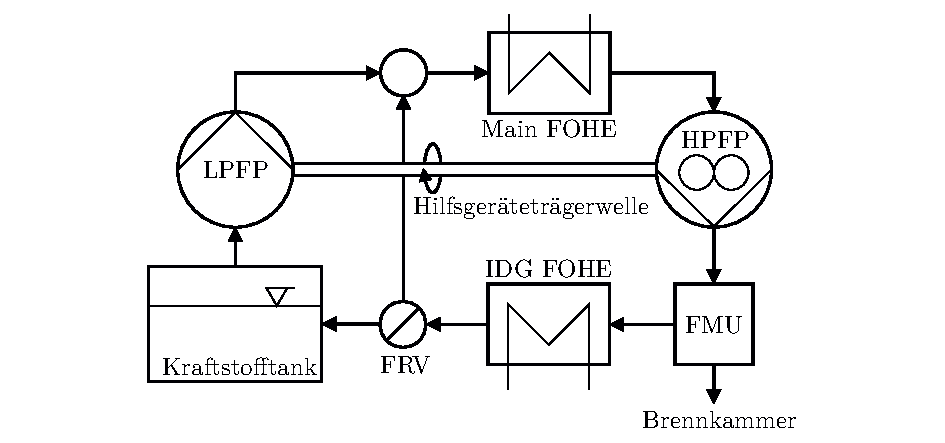
\includegraphics[width=1\linewidth]{4_Abbildungen/2_Hauptteil/Kraftstoffsystem Abbildungen/CFM56 Kraftstoffsystem 2.pdf}
  \caption{Kraftstoffsystems des CFM56-5B Triebwerks nach \cite{LinkeDiesinger.2014}}
  \label{fig:2.1}
\end{figure}
\FloatBarrier

Die in den Kraftstofftanks integrierten Boosterpumpen (in Abbildung \ref{fig:2.1} nicht abgebildet) versorgen die Triebwerke mit Kraftstoff. Im CFM56-5B Triebwerk wird der Kraftstoff zunächst von der Niederdruckpumpe in das Niederdrucksystem gefördert. Anschließend erfolgt eine Mischung mit warmem, rezirkuliertem Kraftstoff aus dem Hochdrucksystem. Nachdem der Kraftstoff in einem Wärmeübertrager für das Hauptölsystem weiter erwärmt wurde, durchläuft er den Kraftstofffilter und die Hochdruckpumpe.

Der Filter des CFM56-5B Triebwerks ist branchenüblich mit einem von einem Druckdifferenzsensor gesteuerten Bypass-Ventil ausgestattet, das im Falle einer Verstopfung aktiviert wird. Der Kraftstoffmassenstrom und -druck in die Brennkammer werden durch die Kraftstoffregeleinheit gesteuert, die im CFM56-5B Triebwerk auch als hydromechanische Einheit (engl.: Hydromechanical Unit, HMU) bezeichnet wird. Überschüssiger Kraftstoff durchläuft zunächst den Wärmeübertrager des Stromgenerator-Ölsystems und erreicht anschließend das Kraftstoff-Rückführventil (engl.: Fuel Return Valve, FRV). Je nach Öltemperatur bestimmt das Wärmemanagementsystem des CFM56-5B Triebwerks anhand eines Kennfeldes, welcher Kraftstoffmassenstrom in die Kraftstofftanks zurückgeleitet wird. Der restliche Kraftstoff wird in das Niederdrucksystem zurückgeführt. Die Kraftstofftemperatur wird vom Wärmemanagementsystem des CFM56-5B Triebwerk nicht berücksichtigt. \cite{Braunling.2015, LinkeDiesinger.2014}

\section{Wasserstoff-Kraftstoffsysteme}

Die Kraftstoffsysteme wasserstoffbetriebener Triebwerke müssen viele der gleichen Funktionen wie Kerosin-Kraftstoffsysteme erfüllen. Aufgrund der abweichenden Kraftstoffeigenschaften ergeben sich jedoch spezifische Herausforderungen. Da der Wasserstoff für Luftfahrtanwendungen in flüssiger, also kryogener Form bei niedrigen Temperaturen gespeichert wird, stellt die Vorkonditionierung eine besondere Herausforderung dar. Die Kombination aus niedrigeren Lagertemperaturen und der hohen spezifischen Wärmekapazität von Wasserstoff führt zu einem hohen Energiebedarf. \cite{Rompokos.2024, Sethi.2022}

Aus diesem Grund werden in der Literatur neben den aus konventionellen Kraftstoffsystemen bekannten Wärmeübertragern mit den Ölsystemen auch Wärmeübertrager innerhalb des thermodynamischen Kreisprozesses des Triebwerks untersucht (siehe Abbildung \ref{fig:2.2}). Diese sogenannten fortschrittlichen Kreisprozesse könnten nicht nur zusätzliche Wärmeeinträge in das Kraftstoffsystem liefern, sondern auch den Gesamtwirkungsgrad des Triebwerks steigern \cite{Tacconi.2023}.

\begin{figure}[ht]
\centering
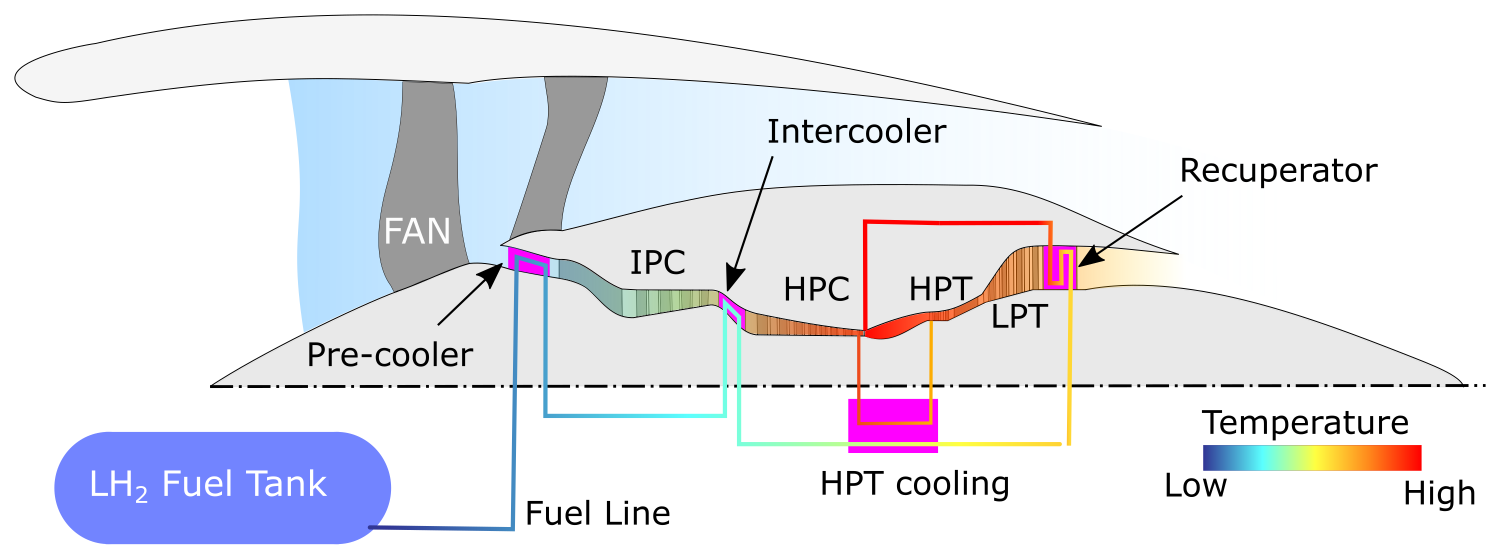
\includegraphics[width=0.75\linewidth]{4_Abbildungen/2_Hauptteil/Advanced Cycles.png}
  \caption{Wärmeübertrager fortschrittlicher Kreisprozesse \cite{Sethi.2022}}
  \label{fig:2.2}
\end{figure}
\FloatBarrier 

Zu den untersuchten fortschrittlichen Kreisprozessen zählen Vor-/Zwischenkühler, die durch geringere Eintrittstemperaturen der Luft in die Verdichter des Kerntriebwerks deren Arbeitsbedarf reduzieren \cite{Abedi.2022}. Wärmerückgewinnungssysteme im Abgas der Niederdruckturbine, sogenannte Rekuperatoren, senken die Abgastemperatur und erhöhen dadurch den Gesamtwirkungsgrad des Kreisprozesses \cite{Brewer.1991}. Eine Vorkühlung der Turbinenkühlluft in einem eigenen Wärmeübertrager könnte den benötigten Massenstrom an Kühlluft verringern und so den Turbinenwirkungsgrad steigern \cite{Brewer.1991}. Die Integration dieser Wärmeübertrager in den Kreisprozess des Triebwerks ist jedoch mit erheblichen finanziellen und technischen Risiken verbunden, weshalb ein Einsatz in der ersten Generation wasserstoffbetriebener Flugzeugtriebwerke als unwahrscheinlich gilt \cite{Rompokos.2024, Huete.2021}. 

Da sich diese Arbeit primär mit der Nachrüstung von kerosinbetriebenen Flugtriebwerken für die Nutzung mit Wasserstoff befasst, werden fortschrittliche Kreisprozesse nicht näher betrachtet. Das Wärmemanagement von Wasserstoff-Kraftstoffsystemen hält die Temperaturen der Ölsysteme innerhalb ihrer Betriebsgrenzen und stellt eine Mindesttemperatur des Kraftstoffs sicher. Im Folgenden werden mögliche Komponenten von Wasserstoff-Kraftstoffsystemen diskutiert und eine Kraftstoffsystemarchitektur aus der Literatur beschrieben.

\subsection{Kraftstoffpumpen}

Die Druckerhöhung des Kraftstoffs erfolgt bei den in der Literatur vorgeschlagenen Wasserstoff-Kraftstoffsystemen in zwei Schritten \cite{Ebrahimi.2024}. Für die Niederdruckpumpe wird eine redundante Ausführung in Form von mehreren im Kraftstofftank versenkten Kreiselpumpen vorgeschlagen. Die Niederdruckpumpen des Wasserstoff-Kraftstoffsystems übernehmen die Funktion der Boosterpumpen und der Niederdruckpumpe des Kerosin-Kraftstoffsystems. Aufgrund der physischen Distanz zu den Triebwerkswellen werden diese Pumpen elektrisch angetrieben \cite{Scholz.2003}. 

Für die finale Druckerhöhung gibt es in der Literatur unterschiedliche Ansätze. Das Pumpen von Wasserstoff im flüssigen Zustand erfordert vergleichsweise wenig Energie, jedoch sind Pumpen für kryogenen Wasserstoff aufgrund der unzureichenden Schmierwirkung des Kraftstoffs störanfällig. Bacic et al. \cite{BacicMarkoCoullJohn.2024} schlagen daher vor, den Kraftstoff nach erfolgter Verdampfung zu verdichten, um längere Wartungsintervalle zu ermöglichen. Für die Hochdruckpumpe beziehungsweise den Hochdruckverdichter ist sowohl ein Antrieb über die Hochdruckwelle als auch ein elektrischer Antrieb denkbar. Aufgrund der erforderlichen Druckverhältnisse bei hohem Schubbedarf, erfordert die Verdichtung im gasförmigen Zustand mehrere Verdichterstufen. Für die Druckerhöhung im flüssigen Zustand werden sowohl Kreiselpumpen als auch Verdrängerpumpen diskutiert \cite{Scholz.2003, Shaffer.2014}.

\subsection{Wärmeübertrager}

Neben den aus den Kerosin-Kraftstoffsystemen bekannten Wärmeübertragern mit den Ölsystemen bietet sich aufgrund des niedrigen Temperaturniveaus des flüssigen Wasserstoffs die Integration eines Wärmeübertragers mit dem Kabinen-Klimasystem (engl.: Environmental Control System, ECS) an \cite{Brewer.1991}. Das ECS wird mit Verdichter-Zapfluft versorgt, die vor ihrer Nutzung in der Kabine zunächst abgekühlt wird. In konventionellen Triebwerken wird hierfür ein mit Fan-Zapfluft gekühlter Wärmeübertrager eingesetzt. Durch einen Wärmeübertrager zwischen Wasserstoff und ECS kann der Fan-Zapfluftbedarf reduziert und zusätzliche Wärme für das Wasserstoff-Kraftstoffsystem gewonnen werden. 

Patrao et al. \cite{Patrao.2024} diskutieren die Problematik der Eisbildung in kryogenen Wärmeübertragern im Wasserstoff-Kraftstoffsystem. Ein möglicher Lösungsansatz ist die Rezirkulation des Wasserstoffs innerhalb des Kraftstoffsystems. Hierbei wird warmer Wasserstoff aus dem Hochdrucksystem vor den Eintritt in die betroffenen Wärmeübertrager rezirkuliert, um die Eintrittstemperatur des Wasserstoffs in die Wärmeübertrager so weit zu erhöhen, dass die luftseitigen Temperaturen des Wärmeübertragers stets oberhalb des Gefrierpunkts von Wasser bleiben \cite{Brewer.1991}. 

\subsection{Wärmemanagementsystem}

Das Wärmemanagementsystem von Wasserstoff-Kraftstoffsysteme unterscheidet sich in zwei Kernpunkten von konventionellen Kraftstoffsystemen. Zum einen ist es in der Regel nicht möglich, einen signifikanten Kraftstoffmassenstrom in die Kraftstofftanks rückzuführen, da der rückgeführte Wasserstoff wieder verflüssigt werden müsste. Eine Rückführung des Wasserstoffs für Zwecke des Wärmemanagements ist allerdings auch nicht erforderlich. Im Gegensatz zu Kerosin-Kraftstoffsystemen ist der Kraftstofftemperatur bei den Wasserstoff-Kraftstoffsystemen keine technische Obergrenze gesetzt. Im Gegenteil: Um Vereisungsprobleme aufgrund niedriger Kraftstofftemperaturen in der Brennkammer zu vermeiden, könnte neben der verfügbaren Abwärme auch der Einsatz weiterer Wärmequellen erforderlich sein. Als Alternative zu den zuvor diskutierten fortschrittlichen Kreisprozessen schlagen Palmer et al. \cite{PalmerChloeJWhurrJohnR.2024} vor, die für die Vorkonditionierung benötigte Wärme durch eine mit Fan-Zapfluft versorgte parallele Wasserstoffverbrennung bereitzustellen. Des Weiteren diskutiert der CRYOPLANE-Bericht \cite{Scholz.2003} die Erwärmung des Wasserstoffs im transienten Betrieb mit einer elektrischen Widerstandsheizung.

\subsection{Anordnung der Kraftstoffsystemkomponenten}

Brewer \cite{Brewer.1991} beschreibt in seinem Buch einen denkbaren Ansatz für Wasserstoff-Kraftstoffsysteme. Abbildung \ref{fig:brewer} enthält einen schematische Darstellung der Anordnung der Kraftstoffsystemkomponenten des Kraftstoffsystems von Brewer.


\begin{figure}[ht]
\centering
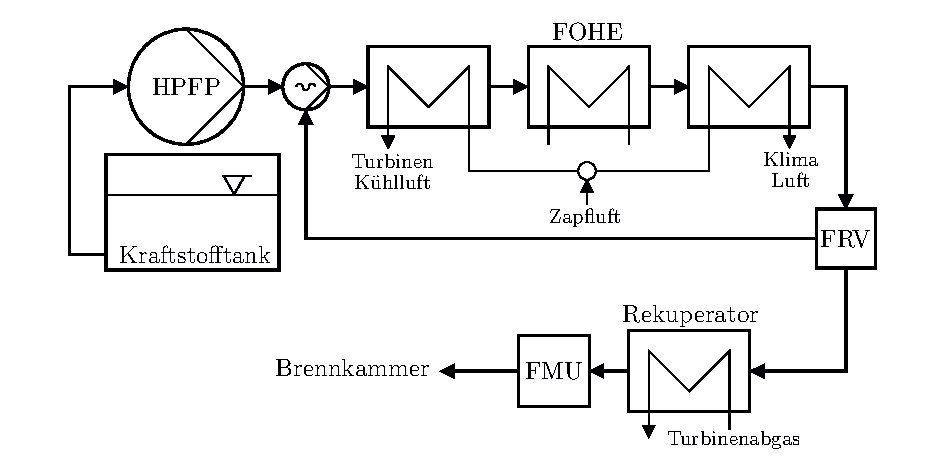
\includegraphics[width=1\linewidth]{4_Abbildungen/2_Hauptteil/Kraftstoffsystem Abbildungen/brewer.pdf}
  \caption{Wasserstoff-Kraftstoffsystem frei nach Brewer \cite{Brewer.1991}}
  \label{fig:brewer}
\end{figure}
\FloatBarrier 

Der flüssige Wasserstoff wird unter Überdruck in einem in die Zelle des Flugzeugs integrierten Kraftstofftank  gelagert. Eine elektrisch angetriebenen Kreiselpumpe fördert den Kraftstoff aus dem Tank in das Triebwerk. Im Triebwerk wird der flüssige Wasserstoff von der Hochdruckpumpe über den Brennkammerdruck gefördert. Im Anschluss an die Hochdruckpumpe, die ebenfalls als Kreiselpumpe ausgeführt ist, wird der geförderte Wasserstoff in einer Strahlpumpe als Treibmedium verwendet, um den rezirkulierten gasförmigen Wasserstoff zu fördern. Der rezirkulierte Wasserstoff gibt Wärme an den flüssigen Wasserstoff ab, wodurch dieser verdampft und auf eine Temperatur von \SI{200}{K} erwärmt wird. 

Der gemischte Wasserstoffstrom durchläuft wird anschließend in einer Reihe von Wärmeübertragern durch die Turbinenkühlluft, das Hauptölsystem und die Klimaluft erwärmt. Hinter den Wärmeübertragern wird der rezirkulierte Massenstrom in einem Kraftstoff-Rückführventil abgezapft. Der verbleibende Kraftstoff durchläuft anschließend einen Rekuperator, der den Wasserstoff auf eine Temperatur von \SI{677}{K} erhitzt. Abschließend wird der Wasserstoff durch die Kraftstoffregeleinheit in die Brennkammer geleitet.
%==============================================================================
\chapter{Methodik}
\label{chap:methodik}
%==============================================================================
Ziel dieser Arbeit ist die Entwicklung einer Methode für die Modellierung von Kraftstoffsystemen von Fluggasturbinen für Schmalrumpfflugzeuge, um deren Auslegung zu unterstützen. Insbesondere wird angestrebt, eine Vergleichbarkeit des Wärme-/Leistungsbedarfs zwischen kerosinbetriebenen und wasserstoffbetriebenen Kraftstoffsystemen zu ermöglichen. 

Hierfür wird zunächst das mathematische Problem der Kraftstoffsysteme formuliert und die Lösung beschrieben. Anschließend wird  das CFM56-5B Triebwerk als Referenzarchitektur nachgebildet und es werden denkbare Architekturen für wasserstoffbetriebene Kraftstoffsysteme erarbeitet. Im nächsten Schritt werden die für die Modellierung der Kraftstoffsysteme notwendigen Komponentenmodelle entwickelt. Abschließend werden die verwendeten Stoffmodelle für die beiden Kraftstoffe beschrieben und sämtliche für die Modellierungen notwendigen Parameter ermittelt.

\section{Annahmen und Vereinfachungen}

Um einen Kompromiss zwischen Detailtiefe, Genauigkeit und Rechenaufwand zu finden, werden in dieser Arbeit mehrere Vereinfachungen verwendet. Insbesondere gelten die betrachteten Modelle lediglich für den stationären Fall. Da der Fokus dieser Arbeit auf der Vorauslegungsrechnung liegt, werden transientes Systemverhalten sowie Off-Design-Verhalten nicht betrachtet. 

Zudem wird in den für die Modellierung relevanten Querschnitten der Kraftstoffsysteme von vernachlässigbaren Geschwindigkeiten, beziehungsweise kinetischen Energien ausgegangen. Innerhalb der modellierten Turbomaschinen ist diese Annahme nicht gültig, jedoch beschränkt sich die Modellierung auf die Erfassung der Größen in den Leitungen zwischen den jeweiligen Komponenten. Bei einer konservativ abgeschätzten Machzahl in den Leitungen $Ma_L=0.1$ und mit dem Isentropenexponenten $\kappa_{\mathrm{H}_2} = 1.4$ beträgt das mit der Isentropenbeziehung berechnete total zu statische Temperaturverhältnis  $\frac{T_{t,L}}{T_L}$

\begin{equation}\label{Eq:mach}
	\frac{T_{t,\mathrm{L}}}{T_\mathrm{L}}=1+\frac{\kappa_{\mathrm{H}_2}-1}{2}Ma_\mathrm{L}^2
\end{equation}

lediglich $1,002$. Unter Annahme eines maximalen Wasserstoffmassenstroms von \SI{0.731}{\kg\per\s} bei einer Temperatur von \SI{300}{\K} beträgt der maximale Leitungsdurchmesser \SI{69}{\milli\m}, was als unkritisch eingestuft wird.

\section{Mathematische Formulierung}

Die Modellierung der Kraftstoffsysteme kann vereinfacht als Funktion $f$ betrachtet werden, welche die unabhängigen Variablen $x$ (Pumpenleistungen, Wärmezufuhr etc.) mithilfe der bekannten Parameter $P$ (Wirkungsgrade, Randbedingungen etc.) auf die abhängigen Variablen $y$ (z.B. Brennkammer-Eintrittstemperatur)

\begin{equation}\label{Eq:fuel_func}
	y = f(x, P)
\end{equation}

abbildet. Zu den Parametern $P$ zählen hierbei beispielsweise als konstant angenommene Pumpenwirkungsgrade und der Ausgangszustand der Kraftstoffe. Für den Zweck dieser Betrachtung fallen unter die unabhängigen Variablen Größen wie der Austrittsdruck der Hochdruckpumpe. Der Brennkammer-Eintrittsdruck und die Brennkammer-Eintrittstemperatur sind Beispiele für die abhängigen Variablen. Für den Zweck dieser Arbeit ist allerdings von Interesse, inwiefern sich die abhängigen Variablen die unabhängigen Variablen auswirken. So ist eine relevante Fragestellung, welche Wärmezufuhr zum erreichen einer bestimmten Brennkammer-Eintrittstemperatur erforderlich ist. Mathematisch entspricht dies der Umkehrfunktion $f^{-1}$, welche die abhängigen Variablen $y$ auf die unabhängigen Variablen $x$

\begin{equation}\label{Eq:fuel_inverse}
	x = f^{-1}(y, P)
\end{equation}

abbildet. Eine analytische Herleitung der Umkehrfunktion der Modellierungen der Kraftstoffsysteme zu bilden, ist nicht möglich. Es ist daher notwendig die Werte der Umkehrfunktion numerisch zu approximieren. Der Lösungsansatz dieser Arbeit für dieses mathematische Problem ist in Abbildung \ref{fig:solver} dargestellt. 

\begin{figure}[ht]
\centering
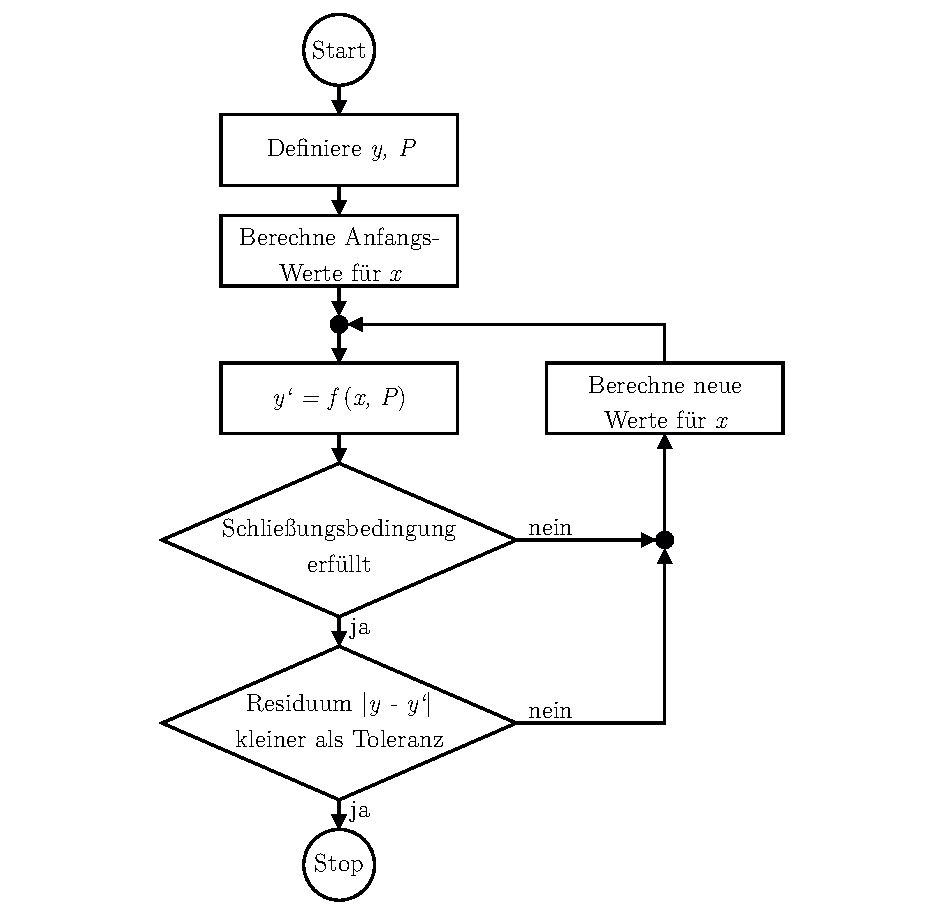
\includegraphics[width=0.8\linewidth]{4_Abbildungen/2_Hauptteil/solver.pdf}
  \caption{Numerische Berechnung von Werten der Umkehrfunktion}
  \label{fig:solver}
\end{figure}
\FloatBarrier 

Zunächst werden die Parameter und die Zielwerte für die abhängigen Variablen definiert. Mithilfe der Zielwerte werden vernünftige Startwerte für die unabhängigen Variablen geschätzt. An dieser Stelle beginnt die iterative Lösung der Modellierung. In jeder Iteration wird mit den gegebenen Werten der unabhängigen Variablen ein Wert für die abhängigen Variablen $y'$ berechnet. Wenn das Residuum, also der Betrag der Differenz zwischen dem Zielwert und dem  berechneten Wert der abhängigen Variable, die Toleranz unterschreitet, ist die Lösung erfolgreich abgeschlossen. Die spezifische Enthalpie der rezirkulierten Kraftstoffmassenströme in dem vorwärts-rechnenden Modell ist unbekannt. Es wird daher mit dem Wert der vorherigen Iteration gerechnet. Dieser Umstand wird durch Einführung einer Schließungsbedingung berücksichtigt. Die Bedingung gilt als erfüllt, wenn der Betrag der Differenz der spezifischen Enthalpien der letzten zwei Iterationen einen geringeren Wert als die Toleranz erreicht.

\section{Referenz-Kraftstoffsystem}

Als Referenzkraftstoffsystem für kerosinbetriebene Triebwerke wird das Kraftstoffsystem des CFM56-5B Triebwerks herangezogen. Die Kraftstoffsysteme der Triebwerke der jüngsten Generation, wie beispielsweise des Pratt \& Whitney PW1133G, sind in der vorhandenen Sachliteratur noch nicht ausführlich dokumentiert. Das andere in der Airbus A320ceo Familie eingesetzte Triebwerk, das IAE V2500-A5 Triebwerk, stellt eine denkbare Alternative dar. Das IAE V2500-A5 ist jedoch nicht gut für die Zwecke einer Modellierung im Rahmen dieser Arbeit geeignet, da das Kraftstoffrückführventil des  Triebwerks Funktionen aufweist, die in der verfügbaren Literatur nicht ausreichend beschrieben sind \cite{LinkeDiesinger.2014}. Als verbleibendes Triebwerk der Airbus A320ceo Familie fällt die Wahl daher auf das CFM56-5B Triebwerk. 

\subsection{Systemarchitektur}

Die Modellierung des Referenzkraftstoffsystems orientiert sich an der vereinfachten Darstellung des Kraftstoffsystems des CFM56-5B Triebwerks in Kapitel \ref{chap:grundlagen}. Eine schematische Darstellung der Modellierung des Referenzkraftstoffsystems ist in Abbildung \ref{fig:Referenz} gegeben.

\begin{figure}[ht]
\centering
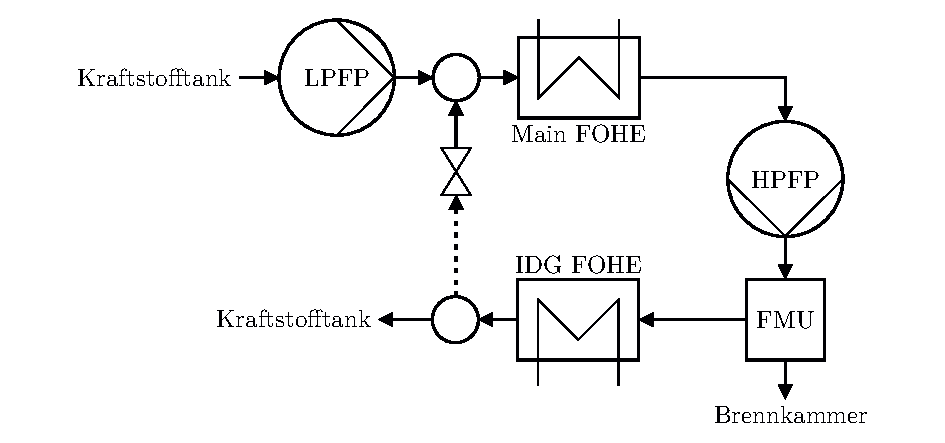
\includegraphics[width=1\linewidth]{4_Abbildungen/2_Hauptteil/Kraftstoffsystem Abbildungen/Referenz.pdf}
  \caption{Referenzkraftstoffsystem}
  \label{fig:Referenz}
\end{figure}
\FloatBarrier 

In dieser Arbeit werden nur Komponenten, die sich innerhalb der Triebwerksgondel befinden, betrachtet. Die Kraftstofftanks und die darin befindlichen Boosterpumpen werden daher nicht modelliert. In der Modellierung wird stattdessen eine Versorgung der Niederdruckpumpe mit dem benötigten Kraftstoffmassenstrom, bei  konstanten Eintrittsbedingungen $T_0, p_0$ angenommen. 

Die Niederdruckpumpe pumpt den Kraftstoff auf einen Austrittsdruck $p_{\mathrm{LPFP}}$ mit einem isentropen Wirkungsgrad $\eta_{\mathrm{LPFP}}$ und einer Leistung $P_{LPFP}$. Da die Modellierung vorwärts rechnet, ist es nicht möglich die spezifische Enthalpie $h_\mathrm{R}$ des rezirkulierten Kraftstoffs direkt innerhalb derselben Iteration zu integrieren. Stattdessen wird die in der vorherigen Iteration berechnete spezifische Enthalpie des rezirkulierten Kraftstoffmassenstroms verwendet. Der rezirkulierte Kraftstoffmassenstrom $\dot{m}_\mathrm{R}$ wird so gewählt, dass die Brennkammer-Eintrittstemperatur $T_{\mathrm{BK}}$ eingehalten wird. 

Der gemischte Kraftstoffmassenstrom durchläuft anschließend den Wärmeübertrager für das Hauptölsystem, nimmt dabei die Wärme $\dot{Q}_{\mathrm{FOHE}}$ auf und erleidet Druckverluste mit dem Druckverhältnis $\pi_{\mathrm{FOHE}}$. Der erwärmte Kraftstoffmassenstrom wird nun in der Hochdruckpumpe mit dem isentropen Wirkungsgrad $\eta_{\mathrm{HPFP}}$ und einer Leistung $P_{\mathrm{HPFP}}$ gepumpt. Der Austrittsdruck der Hochdruckpumpe $p_{\mathrm{HPFP}}$ wird so gewählt, dass der Brennkammer-Eintrittsdruck $p_{\mathrm{BK}}$ erreicht wird. Die Hochdruckpumpe ist als Zahnradpumpe ausgeführt. Da die Hochdruckpumpe für den maximalen Kraftstoffverbrauch im Startfall dimensioniert wird, ist der geförderte Massenstrom im Reiseflug $\dot{m}_{\mathrm{HPFP}}$ vorgegeben. 

Vor dem Eintritt in die Kraftstoffregeleinheit werden in den Leitungen des Kraftstoffsystems auftretende Druckverluste $\Delta p_{\mathrm{L}}$  berücksichtigt. In der Kraftstoffregeleinheit wird der Kraftstoffmassenstrom für die Versorgung der Brennkammer $\dot{m}_{\mathrm{BK}}$ abgezweigt. In den Injektoren erfährt der Kraftstoff den Druckverlust $\Delta p_{\mathrm{inj}}$. 

Der übrige Kraftstoff durchläuft den Wärmeübertrager für das Ölsystem des Stromgenerators und nimmt dabei die Wärme $\dot{Q}_{\mathrm{IDG}}$ auf. Da der rezirkulierte Kraftstoff anschließend gedrosselt wird, wirken sich die Druckverluste dieses Wärmeübertragers nicht auf die Modellierung aus. Nachdem der letzte Wärmeübertrager durchlaufen wurde, wird die spezifische Enthalpie des rezirkulierten Massenstroms berechnet.

\subsection{Variablen und Parameter}

Die abhängigen Variablen des Referenzkraftstoffsystems sind der Brennkammer-Eintrittsdruck $p_{\mathrm{BK}}$ und die Brennkammer-Eintrittstemperatur $T_{\mathrm{BK}}$. Tabelle \ref{Tab:referenz_params} zeigt die Parameter und unabhängigen Variablen des Referenzkraftstoffsystems.

\begin{table}[ht]
    \centering
	\caption{Parameter und Variablen der Modellierung des  Referenzkraftstoffsystems}
	\begin{tabular} {|l|c|l|c|} \hline%
		\multicolumn{2}{|c}{Parameter} & \multicolumn{2}{|c|}{unabhängige Variablen}\\ \hline\hline%
        LPFP-Eintrittstemperatur & $T_0$ & HPFP-Austrittsdruck & $p_{\mathrm{HPFP}}$ \\ \hline
        LPFP-Eintrittsdruck & $p_0$ & HPFP-Leistung & $P_{\mathrm{HPFP}}$ \\ \hline
        FOHE-Wärme & $\dot{Q}_{\mathrm{FOHE}}$ & LPFP-Leistung & $P_{\mathrm{LPFP}}$ \\ \hline
        FOHE-Druckverhältnis & $\pi_{\mathrm{FOHE}}$ & rezirkulierter Massenstrom & $\dot{m}_\mathrm{R}$ \\ \hline
        IDG-FOHE-Wärme  & $\dot{Q}_{\mathrm{IDG}}$ & spezifische Enthalpie von $\dot{m}_\mathrm{R}$ & $h_\mathrm{R}$                 \\ \hline
        LPFP-Austrittsdruck & $p_{\mathrm{LPFP}}$& \multicolumn{2}{c|}{}\\ \hline
        isentroper Wirkungsgrad LPFP & $\eta_{\mathrm{LPFP}}$& \multicolumn{2}{c|}{}\\ \hline
        isentroper Wirkungsgrad HPFP & $\eta_{\mathrm{HPFP}}$& \multicolumn{2}{c|}{}\\ \hline
        HPFP-Massenstrom & $\dot{m}_{\mathrm{HPFP}}$& \multicolumn{2}{c|}{}\\ \hline
        Brennkammermassenstrom & $\dot{m}_{\mathrm{BK},0}$& \multicolumn{2}{c|}{}\\ \hline
        Leitungsdruckverluste & $\Delta p_{\mathrm{L}}$& \multicolumn{2}{c|}{}\\ \hline
        Injektordruckverluste & $\Delta p_{\mathrm{inj}}$& \multicolumn{2}{c|}{}\\ \hline
	\end{tabular}	
    \label{Tab:referenz_params}%
\end{table}
\FloatBarrier 

\section{Wasserstoff-Kraftstoffsystemarchitekturen}

Im folgenden werden unterschiedliche Architekturen für Wasserstoff-Kraftstoffsysteme ausgearbeitet und beschrieben. Abschließend werden die für die Modellierung der Architekturen notwendigen Parameter erläutert. 

Bei den Wasserstoff-Kraftstoffsystemen werden insbesondere zwischen Systemen mit Hochdruckpumpe und Hochdruckverdichter unterschieden. Die Hochdruckpumpe hat den Vorteil eines geringen Leistungsbedarfs, jedoch birgt die Pumpe aufgrund der aufwendigen Schmierung ein höheres Technologierisiko. 

Insgesamt werden drei unterschiedliche Kraftstoffsystemarchitekturen betrachtet. Neben einem Kraftstoffsystem mit Hochdruckpumpe werden zwei Systeme mit Verdichter betrachtet. Die beiden Systeme mit Verdichter unterscheiden sich darin, wie sie den Wasserstoff verdampfen. Bei dem Kraftstoffsystem mit Verdampfer wird der Wasserstoff in einem Wärmeübertrager mit Kraftstoff aus dem Hochdrucksystem verdampft. Bei dem Kraftstoffsystem mit Vormischung wird eine geringe Menge Wasserstoff aus dem Hochdrucksystem vor den Verdichter rezirkuliert, um den Kraftstoff vollständig zu verdampfen.

\subsection{Architektur mit Hochdruckpumpe}

Im Gegensatz zu dem konventionellen Kraftstoffsystem wird bei der Wasserstoff-Kraftstoffsystemarchitektur mit Hochdruckpumpe die Funktion der Pumpe nicht auf eine Hochdruck- und eine Niederdruckpumpe mit Wärmeübertragern dazwischen aufgeteilt. Eine Wärmezufuhr hinter einer möglichen Niederdruckpumpe würde den Wasserstoff schon vor der Hochdruckpumpe verdampfen. Die Lösung besteht darin, den Wasserstoff mit einer einzelnen Kreiselpumpe direkt in das Hochdrucksystem zu pumpen und erst daraufhin Wärme zuzuführen. Die hier diskutierte Kraftstoffsystemarchitektur basiert auf einem von Brewer diskutierten Kraftstoffsystem \cite{Brewer.1991}, jedoch wurden keine Wärmeübertrager mit der Turbinenkühlluft und dem Turbinenabgas vorgesehen. Stattdessen versorgt eine parallele Wasserstoffverbrennung den auftretenden Wärmefehlbetrag zwischen dem Bedarf und der verfügbaren Abwärme. Das Wasserstoff-Kraftstoffsystem mit Pumpe ist in  Abbildung \ref{fig:pumpe} dargestellt.

\begin{figure}[ht]
\centering
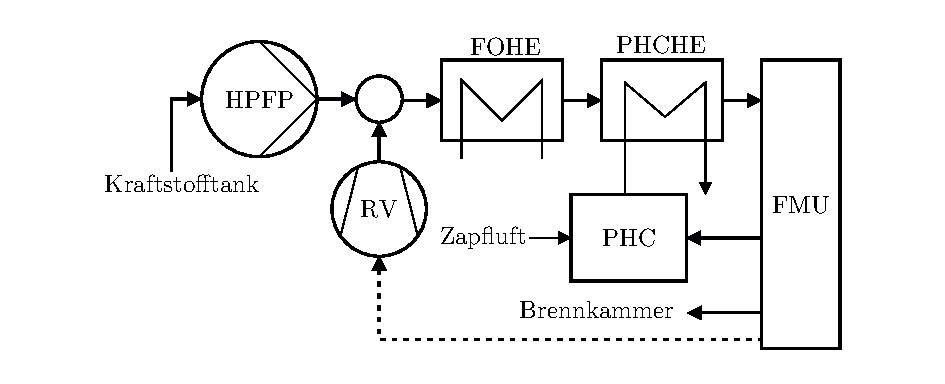
\includegraphics[width=1\linewidth]{4_Abbildungen/2_Hauptteil/Kraftstoffsystem Abbildungen/pump.pdf}
  \caption{Wasserstoffkraftstoffsystem mit Pumpe adaptiert aus \cite{Brewer.1991}}
  \label{fig:pumpe}
\end{figure}
\FloatBarrier 

Der Wasserstoff erreicht das Triebwerk im flüssigen Zustand mit dem Eintrittsdruck $p_0$ und der Eintrittstemperatur $T_0$ und wird direkt in der Hochdruckpumpe auf den Druck $p_{\mathrm{HPFP}}$ gepumpt, sodass der Brennkammer-Eintrittsdruck $p_{\mathrm{BK}}$ erreicht wird. Die Hochdruckpumpe arbeitet mit dem isentropen Wirkungsgrad $\eta_{\mathrm{HPFP}}$ und benötigt die Leistung $P_{\mathrm{HPFP}}$. 

Im Anschluss an die Hochdruckpumpe wird der Kraftstoffmassenstrom $\dot{m}_\mathrm{R}$ mit der spezifischen Enthalpie $h_\mathrm{R}$ dazugemischt. Der warme rezirkulierte Kraftstoff verdampft den flüssigen Kraftstoff und erwärmt diesen auf die Wärmeübertrager-Eintrittstemperatur $T_\mathrm{W}$, um Vereisungen im Ölsystem zu vermeiden.

Auf den Wärmeübertrager mit dem Klimasystem, folgt der Wärmeübertrager mit dem Ölsystem. Der Einfachheit halber werden die beiden Wärmeübertrager in der Modellierung zusammengefasst. In den beiden Wärmeübertragern wird dem Kraftstoff in Summe die Wärme $\dot{Q}_{\mathrm{FOHE}}$ zugeführt. Über die beiden Wärmeübertrager liegt das Druckverhältnis $\pi_{\mathrm{FOHE}}$ vor. Der durch den Wärmeübertrager mit dem Klimasystem gesparte Fan-Zapfluftbedarf wird in der Modellierung nicht berücksichtigt. Um die angestrebte Brennkammer-Eintrittstemperatur $T_{\mathrm{BK}}$ zu erreichen, wird durch eine parallele Wasserstoffverbrennung (engl.: Parallel Hydrogen Combustion, PHC) in einem weiteren Wärmeübertrager (engl.: PHC Heat Exchanger, PHCHE) die zusätzliche Wärme $\dot{Q}_{\mathrm{PHC}}$ zugeführt. Dieser Wärmeübertrager verursacht das Druckverhältnis $\pi_{\mathrm{PHC}}$. 

Vor dem Eintritt in die Kraftstoffregeleinheit werden in den Leitungen des Kraftstoffsystems auftretende Druckverluste $\Delta p_\mathrm{L}$  berücksichtigt. Die Kraftstoffregeleinheit liefert den Kraftstoffmassenstrom $\dot{m}_{\mathrm{BK}}$ an die Hauptbrennkammer und die Brennkammer der parallelen Wasserstoffverbrennung. Der verbleibender Massenstrom $\dot{m}_\mathrm{R}$ mit der Enthalpie $h_\mathrm{R}$ wird rezirkuliert. Vor dem Eintritt in die Brennkammern erfährt der Wasserstoff die Injekor- und Leitungsdruckverluste $\Delta p_{\mathrm{inj}}$. 

Um die Druckverluste im Hochdrucksystem zu kompensieren, schlägt Brewer eine Strahlpumpe mit dem  Hochdruckpumpen-Kraftstoffmassenstrom als Treibmedium vor \cite{Brewer.1991}. Da in dieser Arbeit der rezirkulierte Massenstrom teilweise ein vielfaches des Hochdruckpumpen-Massenstroms beträgt, würde eine Strahlpumpe nicht hinnehmbare Druckverluste verursachen. Stattdessen wird ein Rezirkulationsverdichter (RV) modelliert, der den rezirkulierte Kraftstoff vom Eintrittsdruck $p_\mathrm{R}$ auf den Austrittsdruck der Hochdruckpumpe verdichtet. Der Rezirkulationsverdichter arbeitet mit der Leistung $P_\mathrm{VR}$ und dem isentropen Wirkungsgrad $\eta_\mathrm{RV}$. 

\subsection{Architektur mit Verdampfer}

Die Architektur mit Verdichter und Verdampfer ist ähnlich aufgebaut wie das Kraftstoffsystem mit Hochdruckpumpe, jedoch wird anstatt der Hochdruckpumpe ein Hochdruckverdichter (engl.: High Pressure Fuel Compressor, HPFC) eingesetzt. Bevor der Kraftstoffmassenstrom den Verdichter erreicht, wird er in einem Wärmeübertrager mit Wärme aus dem Hochdrucksystem verdampft. Das Kraftstoffsystem mit Verdampfer ist in Abbildung \ref{fig:verdampfer} dargestellt.

\begin{figure}[ht]
\centering
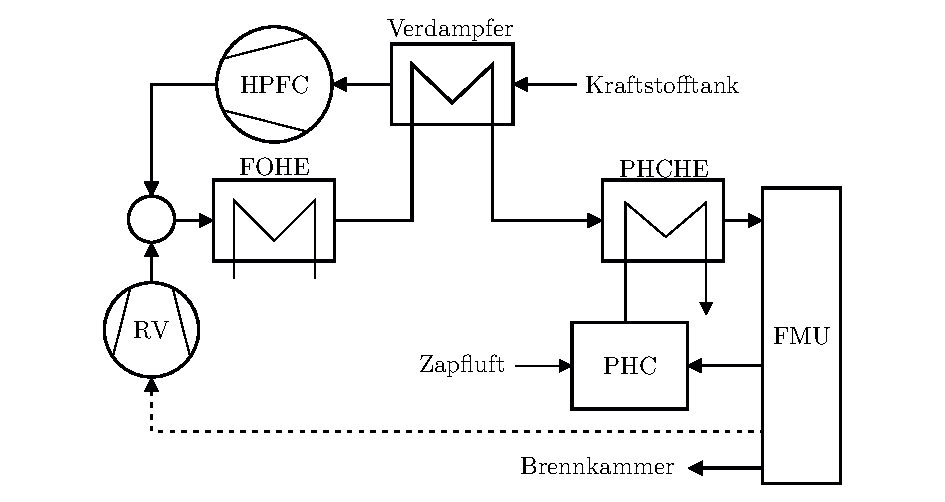
\includegraphics[width=1\linewidth]{4_Abbildungen/2_Hauptteil/Kraftstoffsystem Abbildungen/after.pdf}
  \caption{Wasserstoffkraftstoffsystem mit Verdichter und Verdampfer}
  \label{fig:verdampfer}
\end{figure}
\FloatBarrier 

Der Wasserstoff wird in dem Triebwerk zunächst in dem Verdampfer unter Zuführung des Wärmestroms $|\dot{Q}_\mathrm{V}|$ aus dem Hochdrucksystem gerade vollständig verdampft. Hierbei liegt über die Niederdruckseite des Wärmeübertragers das Druckverhältnis $\pi_{\mathrm{V,LP}}$ an. Der Hochdruckverdichter fördert den Wasserstoff mit dem Druck $p_{\mathrm{HPFC}}$ in das Hochdrucksystem, sodass der Brennkammer-Eintrittsdruck $p_{\mathrm{BK}}$ erreicht wird. Der Hochdruckverdichter arbeitet mit dem isentropen Wirkungsgrad $\eta_{\mathrm{HPFC}}$ und benötigt die Leistung $P_{\mathrm{HPFC}}$. 

Die Hochdruckseite gleicht dem Kraftstoffsystem mit Hochdruckpumpe mit dem einzigen Unterschied, dass zwischen den Wärmeübertragern mit dem Klima-/Ölsystem und dem Wärmeübertrager der parallelen Wasserstoffverbrennung die Hochdruckseite des Verdampfers durchlaufen wird. Hier wird die Wärme $\dot{Q}_\mathrm{V}$ an das Niederdrucksystem abgegeben und es liegt das Druckverhältnis $\pi_{\mathrm{V,HP}}$ an. Der Verdampfer wird auf der Hochdruckseite vor dem Wärmeübertrager mit der parallelen Wasserstoffverbrennung positioniert, um die maximale Wasserstofftemperatur zu mindern. Die geringere Maximaltemperatur ermöglicht eine geringere Abgastemperatur der parallelen Wasserstoffverbrennung und reduziert somit ihren Wasserstoffverbrauch.

\subsection{Architektur mit Vormischung}

Dieses Kraftstoffsystem zeichnet sich dadurch aus, dass an zwei unterschiedliche Positionen Kraftstoff von der Kraftstoffregeleinheit rezirkuliert wird. Zum einen wie auch bei den anderen Wasserstoff-Kraftstoffsystemen über einen Rezirkulationsverdichter hinter den Hochdruckverdichter. Ein kleiner rezirkulierter Kraftstoffmassenstrom $\dot{m}_\mathrm{V}$ wird stattdessen gedrosselt und vor den Hochdruckverdichter rezirkuliert, um den aus dem Kraftstofftank geförderten Wasserstoff ohne den Einsatz zusätzlicher Wärmeübertrager zu verdampfen. Das Hochdrucksystem ist identisch zu dem Hochdrucksystem des Kraftstoffsystems mit Hochdruckpumpe (Siehe Abbildung \ref{fig:vormischung}).

\begin{figure}[ht]
\centering
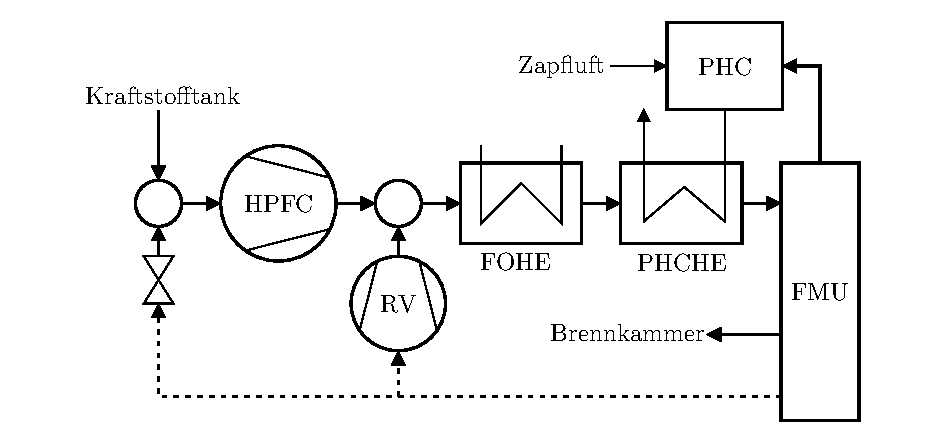
\includegraphics[width=1\linewidth]{4_Abbildungen/2_Hauptteil/Kraftstoffsystem Abbildungen/dual.pdf}
  \caption{Wasserstoffkraftstoffsystem mit Verdichter und Vormischung}
  \label{fig:vormischung}
\end{figure}
\FloatBarrier 

\subsection{Variablen und Parameter}

Die abhängigen Variablen der Modellierungen der Wasserstoff-Kraftstoffsysteme sind der Brennkammer-Eintrittsdruck $p_{\mathrm{BK}}$, die Brennkammer-Eintrittstemperatur $T_\mathrm{BK}$ und die Wärmeübertrager-Eintrittstemperatur $T_\mathrm{W}$. Die Parameter und unabhängigen Variablen der Modellierungen sind in Tabelle \ref{Tab:h2_params} zusammengefasst.

\begin{table}[ht]
    \centering
	\caption{Variablen der Modellierungen der Wasserstoff-Kraftstoffsysteme}
	\begin{tabular} {|l|c|l|c|} \hline%
    \multicolumn{4}{|c}{Alle Wasserstoff-Kraftstoffsysteme}\\ \hline
    \multicolumn{2}{|c}{Parameter} & \multicolumn{2}{|c|}{unabhängige Variablen}\\ \hline\hline%
    isentroper Wirkungsgrad RV & $\eta_\mathrm{RV}$ & RV-Leistung & $P_{\mathrm{RV}}$ \\ \hline
    Kraftstoff-Eintrittsdruck & $p_0$ & rezirkulierter Massenstrom & $\dot{m}_\mathrm{R}$ \\ \hline
    Kraftstoff-Eintrittstemperatur & $T_0$ & Enthalpie des rezirkulierten H$_2$ & $h_\mathrm{R}$ \\ \hline
    PHCHE-Druckverhältnis  & $\pi_{\mathrm{PHC}}$ & Druck des rezirkulierten H$_2$ & $p_\mathrm{R}$\\ \hline
    FOHE-Wärme & $\dot{Q}_{\mathrm{FOHE}}$ & PHCHE-Wärme  & $\dot{Q}_{\mathrm{PHC}}$\\ \hline
    FOHE-Druckverhältnis & $\pi_{\mathrm{FOHE}}$ & \multicolumn{2}{c|}{}\\ \hline
    Brennkammer-Massenstrom & $\dot{m}_{\mathrm{BK},0}$ & \multicolumn{2}{c|}{}\\ \hline
    Leitungs-Druckverluste & $\Delta p_{\mathrm{L}}$ & \multicolumn{2}{c|}{}\\ \hline
    Injektor-Druckverluste & $\Delta p_{\mathrm{inj}}$ & \multicolumn{2}{c|}{}\\ \hline\hline
	\multicolumn{4}{|c|}{Architektur mit Hochdruckpumpe}\\ \hline
    \multicolumn{2}{|c}{Parameter} & \multicolumn{2}{|c|}{unabhängige Variablen}\\ \hline\hline%
    isentroper Wirkungsgrad HPFP & $\eta_{\mathrm{HPFP}}$ & HPFP-Austrittsdruck & $p_{\mathrm{HPFP}}$ \\ \hline
    & & HPFP-Leistung & $P_{\mathrm{HPFP}}$ \\ \hline\hline
    \multicolumn{4}{|c|}{Architektur mit Verdampfer}\\ \hline
    \multicolumn{2}{|c}{Parameter} & \multicolumn{2}{|c|}{unabhängige Variablen}\\ \hline\hline%
    isentroper Wirkungsgrad HPFC & $\eta_{\mathrm{HPFC}}$ & HPFC-Austrittsdruck & $p_{\mathrm{HPFC}}$ \\ \hline
    Druckverhältnis LP-Verdampfer & $\pi_{\mathrm{V,LP}}$ & HPFC-Leistung & $P_{\mathrm{HPFC}}$ \\ \hline
    Druckverhältnis HP-Verdampfer & $\pi_\mathrm{V,HP}$ & Verdampfer-Wärme & $|\dot{Q}_\mathrm{V}|$ \\ \hline\hline
    \multicolumn{4}{|c|}{Architektur mit Vormischung}\\ \hline
    \multicolumn{2}{|c}{Parameter} & \multicolumn{2}{|c|}{unabhängige Variablen}\\ \hline\hline%
    isentroper Wirkungsgrad HPFC & $\eta_{\mathrm{HPFC}}$ & HPFC-Austrittsdruck & $p_{\mathrm{HPFC}}$ \\ \hline
    \multicolumn{2}{|c|}{}& HPFC-Leistung & $P_{\mathrm{HPFC}}$ \\ \hline
    \multicolumn{2}{|c|}{}& Massenstrom Verdampfung & $\dot{m}_\mathrm{V}$ \\ \hline
    \end{tabular}	
    \label{Tab:h2_params}%
\end{table}
\FloatBarrier 

\section{Modellierung der Komponenten}

Im Folgenden werden die Modellierungen der verschiedenen Komponenten erläutert, die in den Kraftstoffsystemen zum Einsatz kommen. Neben Modellen für Verdichter und Pumpen wird ein Modell für die Wärmeübertrager benötigt. Für die Modellierung der Wasserstoff-Kraftstoffsysteme ist zusätzlich ein Modell für die parallele Wasserstoffverbrennung erforderlich. Darüber hinaus werden die Korrektur des Kraftstoffmassenstroms in Abhängigkeit von der Brennkammereintrittstemperatur sowie für die Hochdruckwellen-Leistungsentnahme beschrieben.

\subsection{Pumpen und Verdichter}

Sämtliche Verdichter- und Pumpentypen werden durch die Definition des isentropen Wirkungsgrad $\eta_s$

\begin{equation}\label{Eq:isentropic}
	\eta_s=\frac{h_2-h_1}{h_{2,s}-h_1}
\end{equation}

modelliert. Dabei werden neben dem isentropen Wirkungsgrad auch der Austrittsdruck $p_2$, der Eintrittsdruck $p_1$, die Eintrittstemperatur $T_1$ und somit die spezifische Eintrittsenthalpie $h_1(T_1, p_1)$ sowie die spezifische Eintrittsentropie $s_1(T_1, p_1)$ als bekannt vorausgesetzt. Die Austrittstemperatur des reversiblen Prozesses $T_{2,s}$ kann iterativ mit der spezifischen Eintrittsentropie $s_1$ und dem Austrittsdruck $p_2$ bestimmt werden. $T_{2,s}$ wird mit der Zustandsgleichung für ideale Gase/Flüssigkeiten unter Annahme einer konstanten spezifischen isobaren Wärmekapazität $c_p$ abgeschätzt. Die Formel für die Differenz der spezifischen Entropie $s(p,T_2)-s(p, T_1)$

\begin{equation}\label{Eq:entropy}
	s(T_2,p)-s(T_1, p)=\cancel{s(T_0,p_0) - s(T_0,p_0)} + c_p(T_1,p) ln\left(\frac{T_2}{T_1}\right) - {\cancel{\overbrace{R ln\frac{p}{p}}^{\substack{\text{Nur bei } \\ \text{idealem Gas}}}}}
\end{equation}

eines ideales Fluids mit zwei unterschiedlichen Temperaturen wird umgestellt, um einen Schätzwert für die Austrittstemperatur des reversiblen Prozesses $T_{2,s}^{n+1}$

\begin{equation}\label{Eq:entropy-temperature}
	T_{2,s}^{n+1}=T_{2,s}^n\mathrm{exp}\left(\frac{s(T_1, p_1)-s(T_{2,s}^n, p_2)}{c_p(T_1, p_1)}\right)
\end{equation}

zu berechnen. Aus der iterativ berechneten Austrittstemperatur ergibt sich die spezifische Austrittsenthalpie $h_{2,s}$ des reversiblen Prozesses und aus Gleichung \ref{Eq:isentropic} folgt direkt die spezifische Austrittsenthalpie des realen Prozesses $h_2$. Anschließend wird mit der spezifischen Austrittsenthalpie und dem Austrittsdruck $p_2$ iterativ die Austrittstemperatur des realen Prozesses $T_2$ bestimmt. Die Formel für die Differenz der spezifischen Enthalpie $h(T_2,p)-h(T_1,p)$

\begin{equation}\label{Eq:enthalpy}
	h(T_2,p)-h(T_1,p)=\cancel{h(T_0,p_0) - h(T_0,p_0)} + c_p(T_1,p)(T_2 - T_1) - {\cancel{\overbrace{v(p-p)}^{\substack{\text{Nur bei idealer} \\ \text{Flüssigkeit}}}}}
\end{equation}

eines ideales Fluids mit zwei unterschiedlichen Temperaturen wird umgestellt, um einen Schätzwert für die Austrittstemperatur des realen Prozesses $T_2^{n+1}$

\begin{equation}\label{Eq:enthalpy-temperature}
	T_2^{n+1}=T_2^n+\frac{h_2-h(T_2^n,p_2)}{c_p(T_2^n,p_2)}
\end{equation}

zu berechnen. Abschließend wird die Verdichter-/Pumpenleistung $P$ 

\begin{equation}\label{Eq:power}
	P=\dot{m}(h_2-h_1)
\end{equation}

für den Kraftstoffmassenstrom $\dot{m}$ über die Energiebilanz um die Komponente bestimmt.

\subsection{Wärmeübertrager}

Da für die Zwecke dieser Modellierung ein stationärer Prozess im Designpunkt des Triebwerks angenommen wird, ist eine ausführliche Modellierung des Wärmeübergangs nicht notwendig. Eine Auslegungsrechnung der Wärmeübertrager wird in dieser Arbeit nicht angestrebt. Die einzige Erfordernis ist, dass die Wärmequelle der Wärmeübertrager in jedem Schnitt ein höheres Temperaturniveau als der Kraftstoffmassenstrom aufweist. Anhand des $\dot{H}-T$ Diagramms (Beispiel siehe Abbildung \ref{fig:hx}) kann festgestellt werden, ob über den gesamten Wärmeübertrager eine minimale Temperaturdifferenz $\Delta T_{min}$ zwischen Wärmequelle und Kraftstoffstrom eingehalten werden kann.


\begin{figure}[ht]
\centering
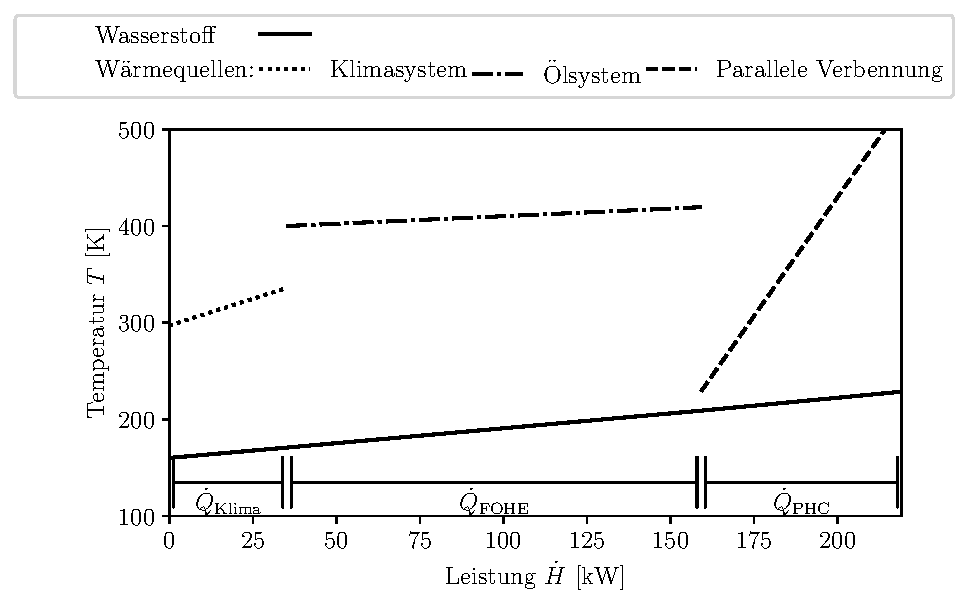
\includegraphics[width=1\linewidth]{4_Abbildungen/2_Hauptteil/hx.pdf}
  \caption{Wärmestromdiagramm für ein Wasserstoffkraftstoffsystem}
  \label{fig:hx}
\end{figure}
\FloatBarrier 

 Aus dem Eintrittszustand des Kraftstoffs in den Wärmeübertrager $T_1, p_1$ ergibt sich die spezifische Enthalpie des Kraftstoff im Eintritt in den Wärmeübertrager $h_1$. Die spezifische Austrittsenthalpie $h_2$

\begin{equation}\label{Eq:energy-hx}
	h_2=h_1 +q=h_1+\frac{\dot{Q}}{\dot{m}}
\end{equation}

erschließt sich direkt aus der Energiebilanz um die Kraftstoffseite des Wärmeübertragers mit dem Wärmestrom $\dot{Q}$ und dem Kraftstoffmassenstrom $\dot{m}$. Über den Wärmeübertrager besteht infolge von Strömungsverlusten ein Druckverhältnis $\pi$. Der Austrittsdruck $p_2$

\begin{equation}\label{Eq:pressuredrop}
	p_2 = p_1 \pi
\end{equation}

fällt somit geringer als der Eintrittsdruck aus. Für die Zwecke dieser Arbeit stellt das Druckverhältnis eine Auslegungsgröße dar und wird daher im Betriebspunkt als konstanten Wert angenommen. Abschließend wird Gleichung \ref{Eq:enthalpy-temperature} erneut eingesetzt, um iterativ die Austrittstemperatur $T_2$ des Kraftstoffs aus dem Wärmeübertrager zu bestimmen.

\subsection{Kraftstoffmischung}

In der Kraftstoffmischung werden die Kraftstoffmassenströme $\dot{m}_{1,\mathrm{\rom{1}}}$ und $\dot{m}_{1,\mathrm{\rom{2}}}$, mit demselben Eintrittsdruck $p_1$, aber unterschiedlichen Eintrittsenthalpien $h_{1,\mathrm{\rom{1}}}, h_{1,\mathrm{\rom{2}}}$ miteinander vermischt. Der Austrittsmassenstrom $\dot{m}_2$

\begin{equation}\label{Eq:mass}
	\dot{m}_2 = \dot{m}_{1,\mathrm{\rom{1}}}+\dot{m}_{1,\mathrm{\rom{2}}}
\end{equation}

berechnet sich aus der Massenbilanz um die Mischung. Die Austrittsenthalpie der Kraftstoffmischung 

\begin{equation}\label{Eq:energy-mix}
	h_{2} = \frac{\dot{m}_{1,\mathrm{\rom{1}}}h_{1,\mathrm{\rom{1}}}+\dot{m}_{1,\mathrm{\rom{2}}}h_{1,\mathrm{\rom{2}}}}{\dot{m}_2}
\end{equation}

wird mit der Energiebilanz um die Mischung bestimmt.  Druckverluste in der Mischung werden vernachlässigt, somit entspricht der Austrittsdruck $p_2$, dem Eintrittsdruck $p_1$. Abschließend wird Gleichung \ref{Eq:enthalpy-temperature} erneut eingesetzt, um iterativ die Austrittstemperatur $T_2$ des gemischten Kraftstoffmassenstroms zu bestimmen. 

\subsection{Parallele Wasserstoffverbrennung}

In den Wasserstoff-Kraftstoffsystemen ist nicht ausreichend Abwärme vorhanden, um den Wasserstoff auf beliebige Brennkammer-Eintrittstemperatur zu erwärmen. In dieser Arbeit wird der zusätzlicher Wärmebedarf durch parallele Wasserstoffverbrennung in einer separaten Brennkammer aufgebracht. Die Brennkammer wird mit Wasserstoff von der Kraftstoffregeleinheit und mit Fan-Zapfluft versorgt. Ziel der Modellierung der parallelen Wasserstoffverbrennung ist es, diesen Mehrbedarf an Wasserstoff und die erforderliche Leistung für die Bereitstellung der Zapfluft zu berechnen. Für diese Betrachtung wird Zapfluft als eine Mischung der idealen Gase Sauerstoff und Stickstoff, mit den spezifischen isobaren Wärmekapazitäten $c_{p,\mathrm{O}_2}, c_{p,\mathrm{N}_2}$ modelliert. Wasserstoff und das durch die Verbrennung erzeugte Wasser werden ebenfalls als ideale Gase mit den Wärmekapazitäten $c_{p,\mathrm{H}_2}, c_{p,\mathrm{H}_2\mathrm{O}}$ modelliert. Zunächst wird das stöchiometrische Sauerstoff/Wasserstoffmassenverhältnis $\frac{\dot{m}_{\mathrm{O}_2, \mathrm{st}}}{\dot{m}_{\mathrm{H}_2,\mathrm{st}}}$ 

\begin{equation}\label{Eq:stoichometric}
	\frac{\dot{m}_{\mathrm{O}_2,\mathrm{st}}}{\dot{m}_{\mathrm{H}_2,\mathrm{st}}}=\frac{M_{R,\mathrm{O}_2}}{2M_{R,\mathrm{H}_2}}
\end{equation}

mit den molaren Massen $M_{R,\mathrm{O}_2}$ und $M_{R,\mathrm{H}_2}$ berechnet. Mit dem Kraftstoff-Luft-Äquivalenz-verhältnis $\phi_{\mathrm{PHC}}$ wird der unverbrannte Sauerstoffmassenstrom $\dot{m}_{\mathrm{B},\mathrm{O}_2}$ 

\begin{equation}\label{Eq:oxygen}
	\frac{\dot{m}_{B,O_2}}{\dot{m}_{H_2}}=\frac{M_{R,O_2}}{2M_{R,H_2}}\left(\frac{1}{\phi_{PHC}}-1\right)
\end{equation}

im Verhältnis zum Wasserstoffmassenstrom $\dot{m}_{\mathrm{H}_2}$ berechnet. Mit dem Sauerstoffmassenanteil in Luft $w_{\mathrm{L, O}_2}$ wird aus Gleichungen \ref{Eq:stoichometric} und \ref{Eq:oxygen} eine Gleichung für den Stickstoffmassenstrom $\dot{m}_{\mathrm{N}_2}$ 

\begin{equation}\label{Eq:nitrogen}
	\frac{\dot{m}_{\mathrm{N}_2}}{\dot{m}_{\mathrm{H}_2}}=\frac{M_{R,\mathrm{O}_2}}{2M_{R,\mathrm{H}_2}}\frac{1-w_{\mathrm{L,O}_2}}{\phi_{\mathrm{PHC}}w_{\mathrm{L,O}_2}}
\end{equation}

im Verhältnis zum Wasserstoffmassenstrom hergeleitet. Nun wird mit der molaren Masse von Wasser $M_{R, \mathrm{H}_2\mathrm{O}}$ die Masse an durch die Verbrennung produziertem Wasser $\dot{m}_{\mathrm{H}_2\mathrm{O}}$

\begin{equation}\label{Eq:water}
	\frac{\dot{m}_{\mathrm{H}_2\mathrm{O}}}{\dot{m}_{\mathrm{H}_2}}=\frac{M_{R,\mathrm{H}_2\mathrm{O}}}{M_{R,\mathrm{H}_2}}
\end{equation}

im Verhältnis zum Wasserstoffmassenstrom berechnet. Anschließend wird die Energiebilanz für die parallele Brennkammer und die Abgasseite des nachgeschalteten Wärmeübertragers aufgestellt. Dabei wird die im Wärmeübertrager abgegebene Wärme $\dot{Q}_{\mathrm{PHC}}$

\begin{equation}\label{Eq:energy-phc}
\begin{multlined}
	\dot{Q}_{\mathrm{PHC}}=(\dot{m}_{\mathrm{N}_2}c_{p,\mathrm{N}_2}+\dot{m}_{\mathrm{B,O}_2}c_{p,\mathrm{O}_2})(T_\mathrm{Z}-T_\mathrm{B})+\dot{m}_{\mathrm{O}_2,\mathrm{st}}\frac{\dot{m}_{\mathrm{H}_2}}{\dot{m}_{\mathrm{H}_2,\mathrm{st}}}c_{p,\mathrm{O}_2}(T_\mathrm{Z}-T_{\mathrm{ref}}) \\
    +\dot{m}_{\mathrm{H}_2}(c_{p,\mathrm{H}_2}(T_{\mathrm{BK}}-T_{\mathrm{ref}})+H_{u,\mathrm{H}_2})-\dot{m}_{\mathrm{H}_2\mathrm{O}}c_{p,\mathrm{H}_2\mathrm{O}}(T_{\mathrm{B}}-T_{\mathrm{ref}})
\end{multlined}
\end{equation}

sowie der untere Heizwert von Wasserstoff $H_{u, \mathrm{H}_2}$ bei der Referenztemperatur $T_{\mathrm{ref}}$ berücksichtigt. Die Eintrittstemperatur der Zapfluft $T_\mathrm{Z}$ wird als bekannt vorausgesetzt, und es wird eine vollständige Verbrennung mit einem Wirkungsgrad von $100\,\%$ angenommen. Die Temperatur der abgekühlten Abgase $T_\mathrm{B}$  

\begin{equation}\label{Eq:deltat}
	T_\mathrm{B} = T_{\mathrm{H}_2}+\Delta T_\mathrm{PHC}
\end{equation}

wird aus der Eintrittstemperatur des kalten Wasserstoffs in den Wärmeübertrager $T_{\mathrm{H}_2}$ und der Temperaturdifferenz $\Delta T_{\mathrm{PHC}}$ berechnet. Um den Wasserstoffbedarf $\dot{m}_{\mathrm{PHC}}$ zu ermitteln, wird die Energiebilanz durch den Wasserstoffmassenstrom geteilt und nach dem Wasserstoffmassenstrom umgestellt

\begin{equation}\label{Eq:phc}
	\dot{m}_{\mathrm{PHC}}=\frac{\dot{Q}_{\mathrm{PHC}}}{
    \begin{aligned}
    \left(\frac{\dot{m}_{\mathrm{N}_2}}{\dot{m}_{\mathrm{H}_2}}c_{p,\mathrm{N}_2}+\frac{\dot{m}_{\mathrm{B,O}_2}}{\dot{m}_{\mathrm{H}_2}}c_{p,\mathrm{O}_2}\right)(T_\mathrm{Z}-T_\mathrm{B})+\frac{\dot{m}_{\mathrm{O}_2,\mathrm{st}}}{\dot{m}_{\mathrm{H}_2,\mathrm{st}}}c_{p,\mathrm{O}_2}(T_\mathrm{Z}-T_{\mathrm{ref}})\\
    +c_{p,\mathrm{H}_2}(T_{\mathrm{BK}}-T_{\mathrm{ref}})-\frac{\dot{m}_{\mathrm{H}_2\mathrm{O}}}{\dot{m}_{\mathrm{H}_2}}c_{p,\mathrm{H}_2\mathrm{O}}(T_\mathrm{B}-T_{\mathrm{ref}})
    \end{aligned}
    }\,.
\end{equation}

Abschließend wird die infolge der Fan-Zapfluftentnahme erforderliche zusätzliche Niederdruckwellen-Leistung $P_\mathrm{Z}$

\begin{equation}\label{Eq:fanpower}
	P_\mathrm{Z} = \frac{\dot{m}_{\mathrm{PHC}}}{\eta_1}\left(\frac{\dot{m}_\mathrm{{N}_2}}{\dot{m}_{\mathrm{H}_2}}c_{p,\mathrm{N}_2}+\left(\frac{\dot{m}_{\mathrm{B,O}_2}}{\dot{m}_{\mathrm{H}_2}}+\frac{\dot{m}_{\mathrm{O}_2,\mathrm{st}}}{\dot{m}_{\mathrm{H}_2,\mathrm{st}}}\right)c_{p,\mathrm{O}_2}\right)(T_\mathrm{Z}-T_\mathrm{U})
\end{equation}

mit der Umgebungstemperatur $T_\mathrm{U}$ und dem mechanischen Wirkungsgrad der Niederdruckwelle $\eta_1$ berechnet. Die Modellierung der parallelen Wasserstoffverbrennung erfordert die in Tabelle \ref{Tab:phc_params} aufgeführten Parameter.

\begin{table}[ht]
    \centering
	\caption{Parameter der Modellierung der parallelen Wasserstoffverbrennung}
	\begin{tabular} {|l|c|} \hline%
    \multicolumn{2}{|c|}{Parameter} \\ \hline\hline
    spezifische isobare Wärmekapazität Sauerstoff & $c_{p, O_2}$ \\ \hline
    spezifische isobare Wärmekapazität Stickstoff & $c_{p, N_2}$ \\ \hline
    spezifische isobare Wärmekapazität Wasserstoff & $c_{p, H_2}$ \\ \hline
    spezifische isobare Wärmekapazität Wasser & $c_{p, \mathrm{H}_2\mathrm{O}}$ \\ \hline
    molare Masse Sauerstoff & $M_{R, \mathrm{O}_2}$ \\ \hline
    molare Masse Wasserstoff & $M_{R, \mathrm{H}_2}$ \\ \hline
    molare Masse Wasser & $M_{R, \mathrm{H}_2\mathrm{O}}$ \\ \hline
    Äquivalenzverhältnis & $\phi_{\mathrm{PHC}}$ \\ \hline
    Sauerstoffmassenanteil & $w_{\mathrm{L,O}_2}$ \\ \hline
    unterer Heizwert Wasserstoff & $H_{u, \mathrm{H}_2}$ \\ \hline
    Referenztemperatur & $T_{\mathrm{ref}}$ \\ \hline
    Zapflufttemperatur & $T_\mathrm{Z}$ \\ \hline
    Umgebungstemperatur & $T_\mathrm{U}$ \\ \hline
    Wirkungsgrad Niederdruckwelle & $\eta_1$ \\ \hline
    Wärmeübertrager Temperaturdifferenz & $\Delta T_{\mathrm{PHC}}$ \\ \hline  
    
	\end{tabular}	
    \label{Tab:phc_params}%
\end{table}
\FloatBarrier 

\subsection{Korrektur des Kraftstoffmassenstroms}

Die Kraftstoffmassenströme $\dot{m}_{\mathrm{BK},0}$ im Reiseflug gelten für Referenz-Kraftstofftemperaturen $T_{\mathrm{ref,H_2}}$ beziehungsweise $T_{\mathrm{ref, Jet-A}}$. Der erforderliche Kraftstoffmassenstrom $\dot{m}_{BK}$

\begin{equation}\label{Eq:tempcorr}
	\dot{m}_{\mathrm{BK}}=\dot{m}_{\mathrm{BK},0}\frac{H_{u,\mathrm{k}}}{H_{u,\mathrm{k}}+h_\mathrm{k}(T_{\mathrm{BK}}, p_{\mathrm{BK}})-h_\mathrm{k}(T_{\mathrm{ref,k}}, p_{\mathrm{BK}})}
\end{equation}

wird entsprechend der tatsächlichen Brennkammereintrittstemperatur des Kraftstoffs mithilfe der jeweiligen Stoffmodelle korrigiert. Veränderungen in der Abgaszusammensetzung des Kreisprozesses werden vernachlässigt.

Um eine Vergleichbarkeit zwischen den Leistungs- und Wärmebedarfen zu ermöglichen, werden die Bedarfe in den zusätzlichen parasitären Kraftstoffverbrauch der jeweiligen Systeme umgerechnet. Der zusätzliche Kraftstoffverbrauch der Wärmebereitstellung ist durch die Modellierung der parallelen Wasserstoffverbrennung bereits berücksichtigt. Der zusätzliche Kraftstoffbedarf infolge der Leistungsentnahme von den Triebwerkswellen $\dot{m}_{BK,P}$

\begin{equation}\label{Eq:powerofftake}
	\dot{m}_{\mathrm{BK,P}}=\frac{P}{\eta_\mathrm{P}\left(H_{u,\mathrm{k}}+h_\mathrm{k}(T_{\mathrm{BK}}, p_{\mathrm{BK}})-h_\mathrm{k}(T_{\mathrm{ref,k}}, p_{\mathrm{BK}})\right)}
\end{equation}

 wird mit einem Ansatz von Scholz et al. \cite{Scholz.2013} berechnet. Hierfür wird der Wirkungsgrad $\eta_\mathrm{P}$ angenommen. Der gesamte geförderte Kraftstoffmassenstrom beträgt somit
 
 \begin{equation}\label{Eq:sum}
	\dot{m}_{\mathrm{k}}=\dot{m}_{\mathrm{BK}}+\dot{m}_{\mathrm{BK,P}}+\overbrace{\dot{m}_{\mathrm{PHC}}}^{\text{nur H}_2}
\end{equation}
 
 Die zusätzlichen erforderlichen Parameter sind in Tabelle \ref{Tab:fuel_corr_params} zusammengefasst.

 \begin{table}[ht]
    \centering
	\caption{Parameter für die Korrektur des Kraftstoffmassenstroms}
	\begin{tabular} {|l|c|} \hline%
    \multicolumn{2}{|c|}{Parameter} \\ \hline\hline
    unterer Heizwert H$_2$ & $H_{u,\mathrm{H}_2}$ \\ \hline
    unterer Heizwert Jet-A & $H_{u,\mathrm{Jet-A}}$ \\ \hline
    Referenztemperatur H$_2$ & $T_{\mathrm{ref, H}_2}$ \\ \hline
    Referenztemperatur Jet-A & $T_{\mathrm{ref, Jet-A}}$ \\ \hline
    Wirkungsgrad Leistungsentnahme & $\eta_\mathrm{P}$ \\ \hline    
	\end{tabular}	
    \label{Tab:fuel_corr_params}%
\end{table}
\FloatBarrier 

\section{Stoffmodelle}

Für die Modellierung der Kraftstoffsysteme sind Stoffmodelle erforderlich, um thermodynamische Zustandsgrößen wie spezifische Enthalpie und Entropie in Abhängigkeit von Temperatur und Druck der Kraftstoffe bestimmen zu können. In diesem Abschnitt werden die für Kerosin und Wasserstoff verwendeten Stoffmodelle erläutert.

\subsection{Wasserstoff Stoffmodell}

Wasserstoff besteht aus zwei unterschiedlichen Kernspin-Isomeren, Parawasserstoff und Orthowasserstoff. Da sich die beiden Spin-Isomer in ihrer Wärmekapazität bei niedrigen Temperaturen stark unterscheiden, muss das Stoffmodell das Verhältnis der Kern-Isomer berücksichtigen. Bei Temperaturen oberhalb von \SI{200}{\K} liegen die Isomere im thermischen Gleichgewicht in einem Verhältnis von 3:1 zwischen Ortho- und Parawasserstoff vor. Flüssiger Wasserstoff besteht im Gleichgewichtszustand hingegen aus nahezu purem Parawasserstoff (Siehe Abbildung \ref{fig:spin}). In Abwesenheit eines Katalysators wird der Gleichgewichtszustand nur langsam erreicht. Daher ist davon auszugehen, dass der ursprünglich kryogen gelagerte Wasserstoff im Kraftstoffsystem nahezu vollständig in Form von Parawasserstoff vorliegt. Für die Parametrierung des Stoffmodells wird daher eine Zusammensetzung aus purem Parawasserstoff angenommen. \cite{Buntkowsky.2022}

\begin{figure}[ht]
\centering
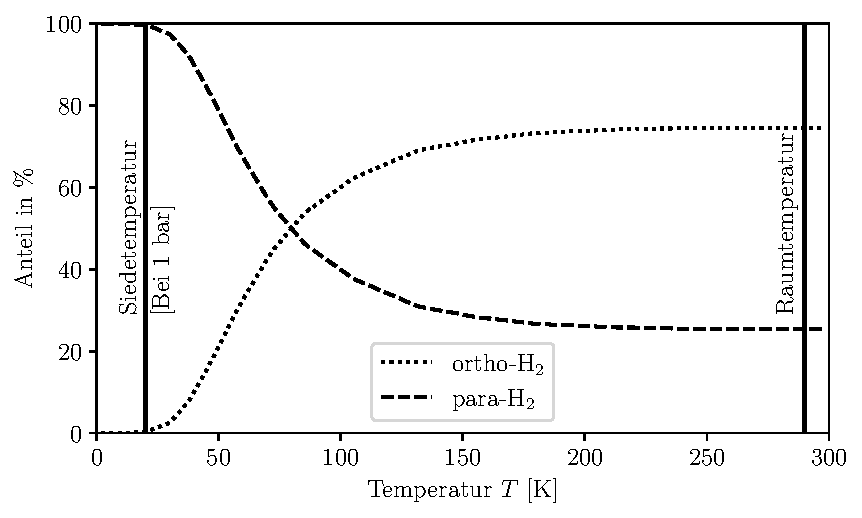
\includegraphics[width=1\linewidth]{4_Abbildungen/2_Hauptteil/spin.pdf}
  \caption{Wasserstoff Kernspin-Isomer Anteile nach \cite{Buntkowsky.2022}}
  \label{fig:spin}
\end{figure}
\FloatBarrier 

Für die Berechnung der thermodynamischen Zustandsgrößen von Parawasserstoff, wird ein am Institut für Strahlantriebe und Turbomaschinen (IST) entwickeltes Stoffmodell weiterentwickelt. Das Stoffmodell basiert auf einem von Leachman et al. \cite{Leachman.2017} beschriebenen Ansatz, der die Zustandsgrößen in Abhängigkeit der Helmholtz-Energie, die auch als freie Energie bekannt ist, setzt. Leachman et al. berechnen die entdimensionierte Helmholtz-Energie $\alpha$ 

\begin{equation}\label{Eq:free-energy}
    \alpha(\delta, \tau) = \alpha^0(\delta, \tau) + \alpha^r(\delta, \tau)
\end{equation}

als Summe der Idealgaskomponente $\alpha^0$ und des Anteils aufgrund von Kompressibilität $\alpha^r$. Hierbei gelten folgende Definitionen der entdimensionierten Helmholtz-Energie $\alpha$ und der entdimensionierten Variablen $\delta$ und $\tau$

\begin{equation}
    \alpha = \frac{a}{RT}, \delta = \frac{\rho}{\rho_c}, \tau = \frac{T_c}{T} \,.
\end{equation}

Mit einer semi-empirischen Zustandsgleichung berechnen Leachman et al die Idealgaskomponente der entdimensionierten freien Energie $\alpha^0$

\begin{equation}\label{Eq:free-energy-idealgas}
    \alpha^0(\tau,\delta)=ln(\delta)+(a_0-1)\mathrm{ln}(\tau)+a_1+a_2\tau-\sum_{i=3}^{m}a_i\frac{(\frac{T_c}{\tau})^{k_i}}{k_i(k_i+1)}+\sum_{i=m+1}^{n}a_i\mathrm{ln}\left(1-e^{\frac{-k_i\tau}{T_c}}\right) \,.
\end{equation}

Die Zustandsgleichung für den Anteil an der entdimensionierten freien Energie aufgrund von Kompressibilitätseffekten $\alpha^r$

\begin{equation}\label{Eq:free-energy-compressibility}
    \alpha^r(\tau,\delta)=\sum_{i=1}^{l}N_i\delta^{d_i}\tau^{t_i}+\sum_{i=l+1}^{m}N_i\delta^{d_i}\tau^{t_i}e^{-\delta^{p_i}}+\sum_{i=m+1}^{n}N_i\delta^{d_i}\tau^{t_i}e^{-\phi_i(\delta-D_i)^2-\beta_i(\tau-\gamma_i)^2)}
\end{equation}

orientiert sich an theoretischen und praktischen Abwägungen. Die in Gleichungen \ref{Eq:free-energy-idealgas} und \ref{Eq:free-energy-compressibility} enthaltenen Parameter werden durch Anpassung auf eine Datenbank experimenteller Daten bestimmt. Da die freie Energie eine Funktion von Dichte und Temperatur ist, der Zustand in dieser Arbeit hingegen in Form von Druck und Temperatur bekannt ist, wird die Dichte zunächst iterativ mithilfe des Newton-Raphson-Verfahrens bestimmt. Mit dem initialen Wert der Dichte $\rho_n$ wird ein Wert für den Druck $p_{\rho_n}$ 

\begin{equation}\label{Eq:pressure-guess}
    p_{\rho_n}=\rho_nRT\left(1+\delta_n\frac{\partial\alpha^r}{\partial\delta}|_{\delta_n, \tau}\right)
\end{equation}

geraten, wobei $\frac{\partial\alpha^r}{\partial\tau}$ mit Gleichung \ref{Eq:free-energy-compressibility} berechnet wird. Anschließend wird mit Gleichung \ref{Eq:pressure-guess} anhand von zwei Stützstellen ein Wert für die Änderungsrate des Drucks $\frac{\mathrm{d}p}{\mathrm{d}\rho}|_{\rho_n,\tau}$ zur Dichte bestimmt. Mithilfe des geratenen Drucks und der Änderungsrate wird der nächste Wert für die Dichte $\rho_{n+1}$

\begin{equation}\label{Eq:density_calc}
    \rho_{n+1}=\rho_n+\frac{p-p_{\rho_n}}{\frac{\mathrm{d}p}{\mathrm{d}\rho}|_{\rho_n,\tau}}
\end{equation}

berechnet. Mit Dichte und Temperatur beziehungsweise deren entdimensionierten Äquivalenten werden die freien Energien und die Ableitungen der freien Energien nach $\delta$ und $\tau$ berechnet. Diese Werte liefern die Grundlage für die Berechnung der notwendigen thermodynamischen Zustandsgrößen mit den in Tabelle \ref{Tab:thermodynamic_properties_h2} definierten Zustandsgleichungen.

\begin{table}[ht]
    \centering
	\caption{Formeln für thermodynamische Zustandsgrößen von Wasserstoff}
	\begin{tabular} {|l|c|c|} \hline%
		\multicolumn{2}{|c|}{Zustandsgröße}  & Formel\\ \hline\hline%
		  spezifische Enthalpie &$h$ 		  & $RT(\tau\frac{\partial\alpha}{\partial\tau}+\delta\frac{\partial\alpha^r}{\partial\delta}+1)$ \\ \hline%
		  spezifische Entropie& $s$ 		      &  $R(\tau\frac{\partial\alpha}{\partial\tau}-\alpha)$\\ \hline%
		spezifische isochore Wärmekapazität &$c_v$ 	    &  $-R\tau^2\frac{\partial^2\alpha}{\partial\tau^2}$\\ \hline%		
        spezifische isobare Wärmekapazität &$c_p$        &  $c_v+R\frac{\left(1+\delta\frac{\partial\alpha^r}{\partial\delta}-\delta\tau\frac{\partial^2\alpha^r}{\partial\delta\partial\tau}\right)^2}{1+2\delta\frac{\partial\alpha^r}{\partial\delta}+\delta^2\frac{\partial^2\alpha^r}{\partial\delta^2}}$\\ \hline%
	\end{tabular}	
    \label{Tab:thermodynamic_properties_h2}%
\end{table}
\FloatBarrier 

\subsection{Kerosin Stoffmodell}

Die Modellierung von Kerosin beziehungsweise Jet-A ist grundsätzlich mit Unsicherheit behaftet, da die Spezifikation des Kraftstoffs vergleichsweise große Abweichungen der Eigenschaften zulässt. Outcalt et al. \cite{Outcalt.2009} haben die Dichte von drei unterschiedlichen Proben an Jet-A Kraftstoff für Temperaturen zwischen \SI{270}{\K} und \SI{470}{\K} und Drücke zwischen \SI{83}{\kilo\Pa} und \SI{30}{\mega\Pa} gemessen und haben eine Abweichung von bis zu $4\,\%$ zwischen den Dichten der Proben ermittelt.

Da Kerosin kein Reinstoff, sondern eine Mischung von Kohlen-Wasserstoffverbindungen mit unterschiedlichen Kettenlängen ist, kann ein Kerosin Stoffmodell nicht mit demselben Ansatz wie das Wasserstoff Stoffmodell entwickelt werden. Stattdessen wird ein empirischer von McBridge et al. \cite{McBridge.2002} vorgeschlagenes Stoffmodell verwendet. Die Autoren haben generische empirische Formeln in Form von Polynomen für die Enthalpie, Entropie und isobare Wärmekapazität aufgestellt und anhand experimenteller Messungen der Zustandsgrößen für 2000 Spezies, inklusive Jet-A Kraftstoff, parametriert. Tabelle \ref{Tab:thermodynamic_properties_jeta} liefert einen Überblick über die verwendeten Zustandsgleichungen.

\begin{table}[ht]
    \centering
	\caption{Thermodynamische Zustandsgrößen von Jet-A Kraftstoff nach 
    \cite{McBridge.2002}}
	\begin{tabular} {|l|c|l|} \hline%
		\multicolumn{2}{|c|}{Zustandsgröße}  & Formel\\ \hline\hline%
		  spezifische Enthalpie &$h$ & $R(a_1T^{-2}+a_2T^{-1} +a_3$ \\ 
        & & $+a_4T+a_5T^2+a_6T^3+a_7T^4)$\\ \hline
		  spezifische Entropie& $s$ &  $R(-a_1T^{-1}+a_2ln(T)+a_3T$\\ 
        & & $+\frac{a_4T^2}{2}+\frac{a_5T^3}{3}+\frac{a_6T^4}{4}+\frac{a_7T^5}{5}+b_1)$\\ \hline
        spezifische isobare Wärmekapazität &$c_p$ &  $R(-\frac{a_1T^{-2}}{2}-a_2T^{-1}+a_3ln(T)+ a_4T$\\ 
	    & & $+\frac{a_5T^{2}}{2}+\frac{a_6T^{3}}{3}+\frac{a_7T^{4}}{4}+b_2)$\\ \hline
    \end{tabular}	
    \label{Tab:thermodynamic_properties_jeta}%
\end{table}
\FloatBarrier 

Da eine Berechnung der Dichte mit demselben Ansatz nicht möglich ist, werden in dieser Arbeit stattdessen die von Outcalt et al. \cite{Outcalt.2009} gemessenen Datenpunkte interpoliert beziehungsweise für Temperaturen unterhalb von \SI{270}{\K} extrapoliert. Als Datengrundlage wird die Probe Jet-A 4658 verwendet, da sie von den Autoren als die repräsentativste der Proben erachtet wird. Für die Berechnung der Dichte $\rho(T,p)$, werden die vier angrenzenden gemessenen Dichten $\rho(T_\mathrm{N},p_{\mathrm{N,n}})$, $\rho(T_\mathrm{N},p_{\mathrm{N,h}})$, $\rho(T_\mathrm{H},p_{\mathrm{H,n}})$ und $\rho(T_\mathrm{H},p_{\mathrm{H,h}})$ benötigt. Bei der Extrapolation werden stattdessen Messwerte der jeweils zwei nächsthöheren Temperaturen als Stützstellen verwendet. Da Outcalt et al. die Dichte für einheitliche Temperaturschritte, aber uneinheitliche Druckschritte gemessen haben, werden zunächst die Dichten $\rho(T_\mathrm{H}, p)$ und $\rho(T_\mathrm{N}, p)$ 

\begin{equation}\label{Eq:pressure-interp}
    \rho(T_i, p)= \rho(T_i, p_{i,\mathrm{n}}) + \frac{\rho(T_i, p_{i,\mathrm{h}})-\rho(T_i, p_{i,\mathrm{n}})}{p_{i,\mathrm{h}}-p_{i,\mathrm{n}}}(p-p_{i,\mathrm{n}}) 
\end{equation}

für den Druck interpoliert. Abschließend wird die Dichte $\rho(T,p)$

\begin{equation}\label{Eq:temperature-interp}
    \rho(T, p)= \rho(T_\mathrm{N}, p) + \frac{\rho(T_\mathrm{H}, p)-\rho(T_\mathrm{N}, p)}{T_\mathrm{H}-T_\mathrm{N}}(T-T_\mathrm{N}) 
\end{equation}

für die Temperatur interpoliert. 								
%==============================================================================
\chapter{Parametrierung}
\label{chap:param}
%==============================================================================

In diesem Kapitel werden die in Kapitel \ref{chap:methodik} definierten physikalischen Modelle der Kraftstoffsysteme parametriert, mit dem Ziel, das Verhalten der Kraftstoffsysteme möglichst realitätsnah abzubilden. Zunächst werden die verwendeten Triebwerkszyklen beschrieben. Hierauf werden die relevanten Parameter bestimmt und deren Herkunft erläutert. Abschließend werden die abhängigen Variablen parametriert und deren Wertebereiche für die Parameterstudie bestimmt.

\section{Triebwerkszyklus}

Die Dimensionierung der Komponenten und die Bestimmung der Randbedingungen der Kraftstoffsysteme erfolgt auf Grundlage von Triebwerkszyklen für moderne wasserstoff-/kerosinbetriebene Getriebefantriebwerke von Schmalrumpfflugzeugen, in Anlehnung an das Pratt \& Whitney PW1133G Triebwerk. Die Betriebspunkte der Triebwerkszyklen wurden am IST mit GasTurb \cite{GasTurbGmbH.2021}, einer Software für die Gasturbinen-Leistungsrechnung, berechnet. Der Betriebspunkt für den Reiseflug wurde für die beiden Zyklen bei einer Flughöhe von \SI{10668}{\m}, einer Machzahl von 0,78, unter Annahme der Internationalen Standardatmosphäre (ISA) und einem Schub von \SI{22}{\kilo\N} gerechnet. Die berechneten Werte sind in Tabelle \ref{Tab:cruise} zusammengefasst.

\begin{table}[ht]
    \centering
	\caption{Betriebspunkt Reiseflug}
	\begin{tabular} {|l|c|c|c|c|} \hline%
    \multicolumn{2}{|c|}{Parameter} & Einheit & H\textsubscript{2} & Kerosin \\ \hline\hline%
    Schub & $F$ & kN & 22 & 22 \\ \hline
    Flughöhe & $H$ & m & 10.668 & 10.668 \\ \hline
    Machzahl & $Ma$ & - & 0,78 & 0,78 \\ \hline
    Umgebungstemperatur & $\Delta T_{\mathrm{ISA}}$ & K & 0 & 0 \\ \hline
    Kraftstoffmassenstrom & $\dot{m}_{\mathrm{BK},0}$& kg/s & 0,10998 & 0,31305 \\ \hline
    Hochdruckwellendrehzahl & $N_2$ & 1/min & 19.376 & 18.647 \\ \hline
    Niederdruckwellendrehzahl & $N_1$ & 1/min & 9153 & 9163 \\ \hline
    Fandrehzahl & $N_\mathrm{F}$ & 1/min & 2989 & 2992 \\ \hline
    Brennkammerdruck & $p_{\mathrm{BK}}$ & kPa & 1330 & 1330 \\ \hline
    Zapflufttemperatur & $T_{\mathrm{Z}}$ & K & 272,63 & - \\ \hline
    Umgebungstemperatur & $T_\mathrm{U}$ & K & 218,81 & - \\ \hline
    Fan-Leistung & $P_\mathrm{F}$ & kW & 6420 & 6420 \\ \hline
    \end{tabular}	
    \label{Tab:cruise}%
\end{table}
\FloatBarrier 

Für die Dimensionierung der Hochdruckpumpe des Referenzkraftstoffsystems ist neben dem Reiseflug auch der Betriebspunkt mit maximalem Startschub (engl.: Maximum Takeoff, MTO) von Interesse. Der Betriebspunkt für den Startfall wurde für den Kerosin-Triebwerkszyklus bei einer Flughöhe von $0$ m, einer Machzahl von $0$, unter Annahme von ISA-Bedingungen und mit dem MTO-Schub von $147,3$ kN gerechnet. Die für die Arbeit relevanten berechneten Werte sind in Tabelle \ref{Tab:mto} gelistet.

\begin{table}[ht]
    \centering
	\caption{Betriebspunkt MTO-Schub}
	\begin{tabular} {|l|c|c|c|} \hline%
    \multicolumn{2}{|c|}{Parameter} & Einheit & Kerosin \\ \hline\hline%
    Schub & $F$ & kN & 147,3 \\ \hline
    Flughöhe & $H$ & m & 0 \\ \hline
    Machzahl & $Ma$ & - & 0 \\ \hline
    Umgebungstemperatur & $\Delta T_{\mathrm{ISA}}$ & K & 0 \\ \hline
    Kraftstoffmassenstrom & $\dot{m}_{\mathrm{BK}}$& kg/s & 1,0540  \\ \hline
    Hochdruckwellendrehzahl & $N_2$ & U/min & 21.099 \\ \hline
    \end{tabular}	
    \label{Tab:mto}%
\end{table}
\FloatBarrier 

\section{Eintrittsbedingungen}

Die Kraftstoff-Eintrittstemperatur in konventionellen Kraftstoffsystemen wird maßgeblich von der Umgebungstemperatur, der verbleibenden Kraftstoffmenge, der Flugdauer sowie der durch Rezirkulation in die Kraftstofftanks rückgeführten Wärme beeinflusst \cite{German.2012}. In dieser Arbeit wird für das Referenzkraftstoffsystem eine Kraftstoffeintrittstemperatur von $T_0=$ \SI{270}{\K} angenommen, was in einer Flughöhe von $H= $ \SI{10668}{\m} einer um \SI{51.3}{\K} höheren Temperatur im Vergleich zur Umgebungstemperatur entspricht. 

Gemäß der Musterzulassung für das Pratt \& Whitney PW1133G-Triebwerk darf der Eintrittsdruck $p_0$ einen Überdruck von \SI{689.47}{\kilo\Pa} relativ zur Umgebung nicht überschreiten und einen Überdruck von \SI{34.47}{\kilo\Pa} relativ zum Dampfdruck des Kraftstoffs nicht unterschreiten \cite{EASA.2018}. Bei einer Kraftstoffeintrittstemperatur $T_0=$ \SI{270}{\K} und einer Flughöhe von \SI{10668}{\m} entspricht dies einem Druckbereich von \SI{35.03}{\kilo\Pa} kPa bis \SI{713.31}{\kilo\Pa}. Durch den Förderdruck der verwendeten Boosterpumpe von ca. \SI{250}{\kilo\Pa} \cite{EatonFuelSystemsDivision.2013} ist dem Kraftstoffeintrittsdruck eine engere Obergrenze gesetzt. Abzüglich Rohrreibungsverlusten in den Kraftstoffleitungen zwischen Kraftstofftank und Triebwerk erscheint ein Eintrittsdruck von $p_0=$ \SI{180}{\kilo\Pa} realistisch.

Das von Brewer \cite{Brewer.1991} vorgeschlagene Kraftstoffsystem, an dem sich die Wasserstoff-Kraftstoffsysteme dieser Arbeit orientieren, verwendet einen Flüssigwasserstofftank mit einem absoluten Druck von \SI{152}{\kilo\Pa} sowie eine im Tank integrierte Niederdruckpumpe, die den flüssigen Wasserstoff auf \SI{462}{\kilo\Pa} fördert. Ähnliche Annahmen treffen die Autoren des CRYOPLANE-Berichts \cite{Scholz.2003}. Unter Berücksichtigung von Druckverlusten erreicht der Wasserstoff das Triebwerk mit einem Eintrittsdruck von $p_0=$ \SI{345}{\kilo\Pa} \cite{Brewer.1991}. Die von Brewer ermittelte Wasserstoff-Eintrittstemperatur $T_0=$ \SI{25.2}{\K} entspricht dem Siedepunkt von Parawasserstoff. In dieser Arbeit wird für den Eintritt eine rein flüssige Wasserstoffphase angenommen.

\section{Abwärmequellen}

Zur Berechnung der in den Wärmeübertragern der Kraftstoffsysteme übertragenen Wärmeströme werden die in den Triebwerken entstehenden Abwärmeströme aufsummiert. Zu den Abwärmequellen moderner Gasturbinentriebwerke zählen neben den Komponenten des Hilfsgeräteträgers insbesondere die Wellenlager sowie, falls vorhanden, das Fan-Getriebe (engl.: Fan Drive Gear System, FDGS). Dem Wasserstoffkraftstoffsystem steht in Form eines Wärmeübertragers mit dem Klimasystem eine zusätzliche Abwärmequelle zur Verfügung. Abbildung \ref{fig:sankey} ist ein Sankey-Diagramm der in konventionellen Kraftstoffsystemen genutzten Abwärmequellen.

\begin{figure}[ht]
\centering
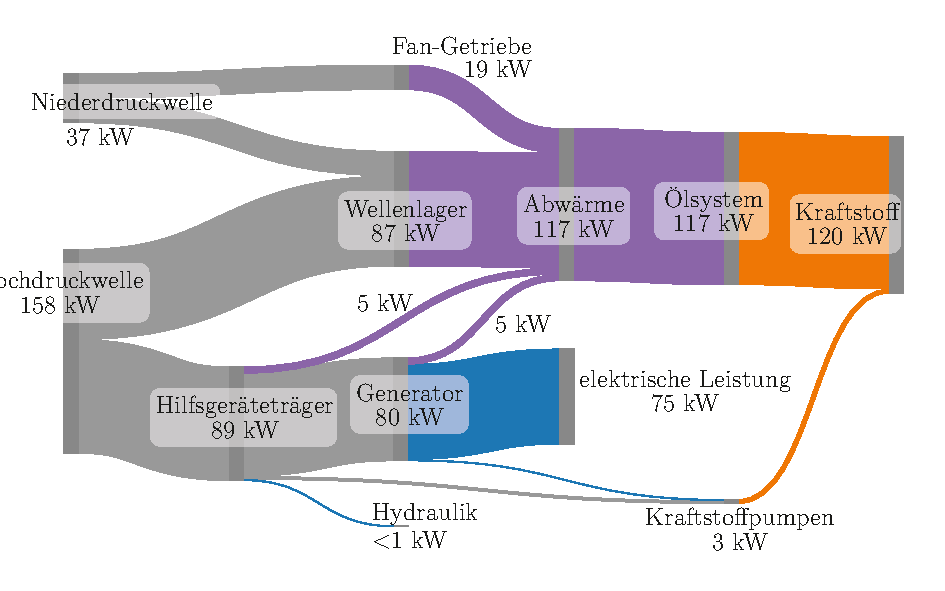
\includegraphics[width=1\linewidth]{4_Abbildungen/2_Hauptteil/sankey.pdf}
  \caption{Abwärmequellen konventioneller Kraftstoffsysteme}
  \label{fig:sankey}
\end{figure}
\FloatBarrier 

\subsection{Wellenlager}

Die Wellenlager sind eine Quelle mechanischer Verluste dar und übertragen die verlorene Leistung nahezu vollständig an das Ölsystem \cite{Gloeckner.2017}. Das PW1133G-Triebwerk ist mit sieben Wellenlagern ausgestattet: Die Hochdruckwelle wird durch ein Fest- und ein Loslager gelagert, die Niederdruckwelle durch ein Fest- und zwei Loslager, und die Fan-Welle wird durch eine angestellte Lagerung gestützt \cite{AviationKnowledge.2022}. 

Die Lagerverluste hängen in erster Linie von der Wellendrehzahl ab, wobei bei Festlagern auch die axiale Belastung der Welle einen Einfluss hat \cite{Zhao.2023}, die in dieser Betrachtung jedoch vernachlässigt wird. Gloeckner et al. \cite{Gloeckner.2017} haben für ein Hochdruckwellenlager bei einer Drehzahl von $19.000$ 1/min einen Leistungsverlust von jeweils \SI{34.8}{\kilo\W} ermittelt. Durch Extrapolation der von Gloeckner \cite{Gloeckner.2013} gemessenen Leistungsverluste einer Lagerung bei $10.000$ 1/min ergibt sich für die Niederdruckwellenlager ein geschätzter Leistungsverlust von jeweils \SI{9}{\kilo\W}. Aufgrund ihrer geringen Drehzahl sind die Leistungsverluste der Fan-Welle vergleichsweise gering. Zhao et al. \cite{Zhao.2023} haben für ein Kugellager in kryogenen Pumpen bei einer Drehzahl von $3000$ 1/min Leistungsverluste von jeweils etwa \SI{0.5}{\kilo\W} berechnet. In Summe betragen die Lagerverlust somit \SI{98}{\kilo\W}.

\subsection{Fan-Getriebe}

Das Fan-Getriebe stellt eine weitere Quelle mechanischer Verluste dar. Pratt \& Whitney erzielte mit dem Getriebe seines Advanced Ducted Propeller (ADP) Demonstrators einen mechanischen Wirkungsgrad von $0,995$ \cite{MCCUNE.1993}. Ein Prototypen-Getriebe des Herstellers aus dem Jahr 1998 soll sogar einen Wirkungsgrad von $0,997$ erreicht haben \cite{anonymous.1998}. Bei einem angenommenen Getriebewirkungsgrad von $0,997$ und einer Fanleistung von \SI{6420}{\kilo\W} (Siehe Tabelle \ref{Tab:cruise}) ergeben sich Leistungsverluste von \SI{19}{\kilo\W}.

\subsection{Hilfsgeräteträger}

Die Kraftstoffpumpen, Ölpumpen, Hydraulikpumpen und der Stromgenerator gehören zu den Hilfsgeräteträger-Komponenten, die erhebliche Abwärme erzeugen. Zusätzlich entstehen durch die Getriebestufen des Hilfsgeräteträgers mechanische Verluste. Jafari et al. \cite{Jafari.2020} haben die Verlustleistung des Hilfsgeräteträgers eines CFM56-5 Triebwerks untersucht und eine Proportionalität zwischen Triebwerksschub und Verlustleistung festgestellt. 

Unter der Annahme dieses Verhaltens beträgt die Verlustleistung des Hilfsgeräteträgers für den betrachteten Triebwerkszyklus \SI{10}{\kilo\W}. Dabei entfällt ein Anteil von \SI{5}{\kilo\W} auf den Stromgenerator. Mögliche erhöhte mechanische Verluste aufgrund des höheren Leistungsbedarfs des Wasserstoffkraftstoffsystems werden aufgrund ihrer geringen Größenordnung als vernachlässigbar betrachtet. 


\subsection{Abwärme}

In Summe wird dem Referenzkraftstoffsystem im Hauptwärmeübertrager eine Wärme von $\dot{Q}_{\mathrm{FOHE}}=$ \SI{122}{\kilo\W} und im Wärmeübertrager des Stromgenerators eine Wärme von $\dot{Q}_{\mathrm{IDG}}=$ \SI{5}{\kilo\W} zugeführt. 

Brewer \cite{Brewer.1991} hat für das Klimasystem eines Schmalrumpfflugzeugs eine Abwärme pro Triebwerk von \SI{32}{\kilo\W} berechnet. Dieser Wert wird für die Modellierung übernommen. Durch das Klimasystem steht den Wasserstoffkraftstoffsystemen eine höhere Abwärme von insgesamt $\dot{Q}_{\mathrm{FOHE}}=$ \SI{159}{\kilo\W} zur Verfügung.

\section{Pumpen und Verdichter}

\subsection{Kreiselpumpen}

Kreiselpumpen kommen im Referenzkraftstoffsystem als Niederdruckpumpe und im Wasserstoffkraftstoffsystem mit Pumpe als Hochdruckpumpe zum Einsatz. Kreiselpumpen erreichen ihren maximalen Wirkungsgrad bei mittleren Volumenströmen und hohen Druckverhältnissen, beziehungsweise Drehzahlen \cite{Gulich.2013}. %Ein typisches Kennfeld einer Kreiselpumpe ist in Abbildung \ref{fig:kreiselpumpe} dargestellt.

%\begin{figure}[ht]
%\centering
%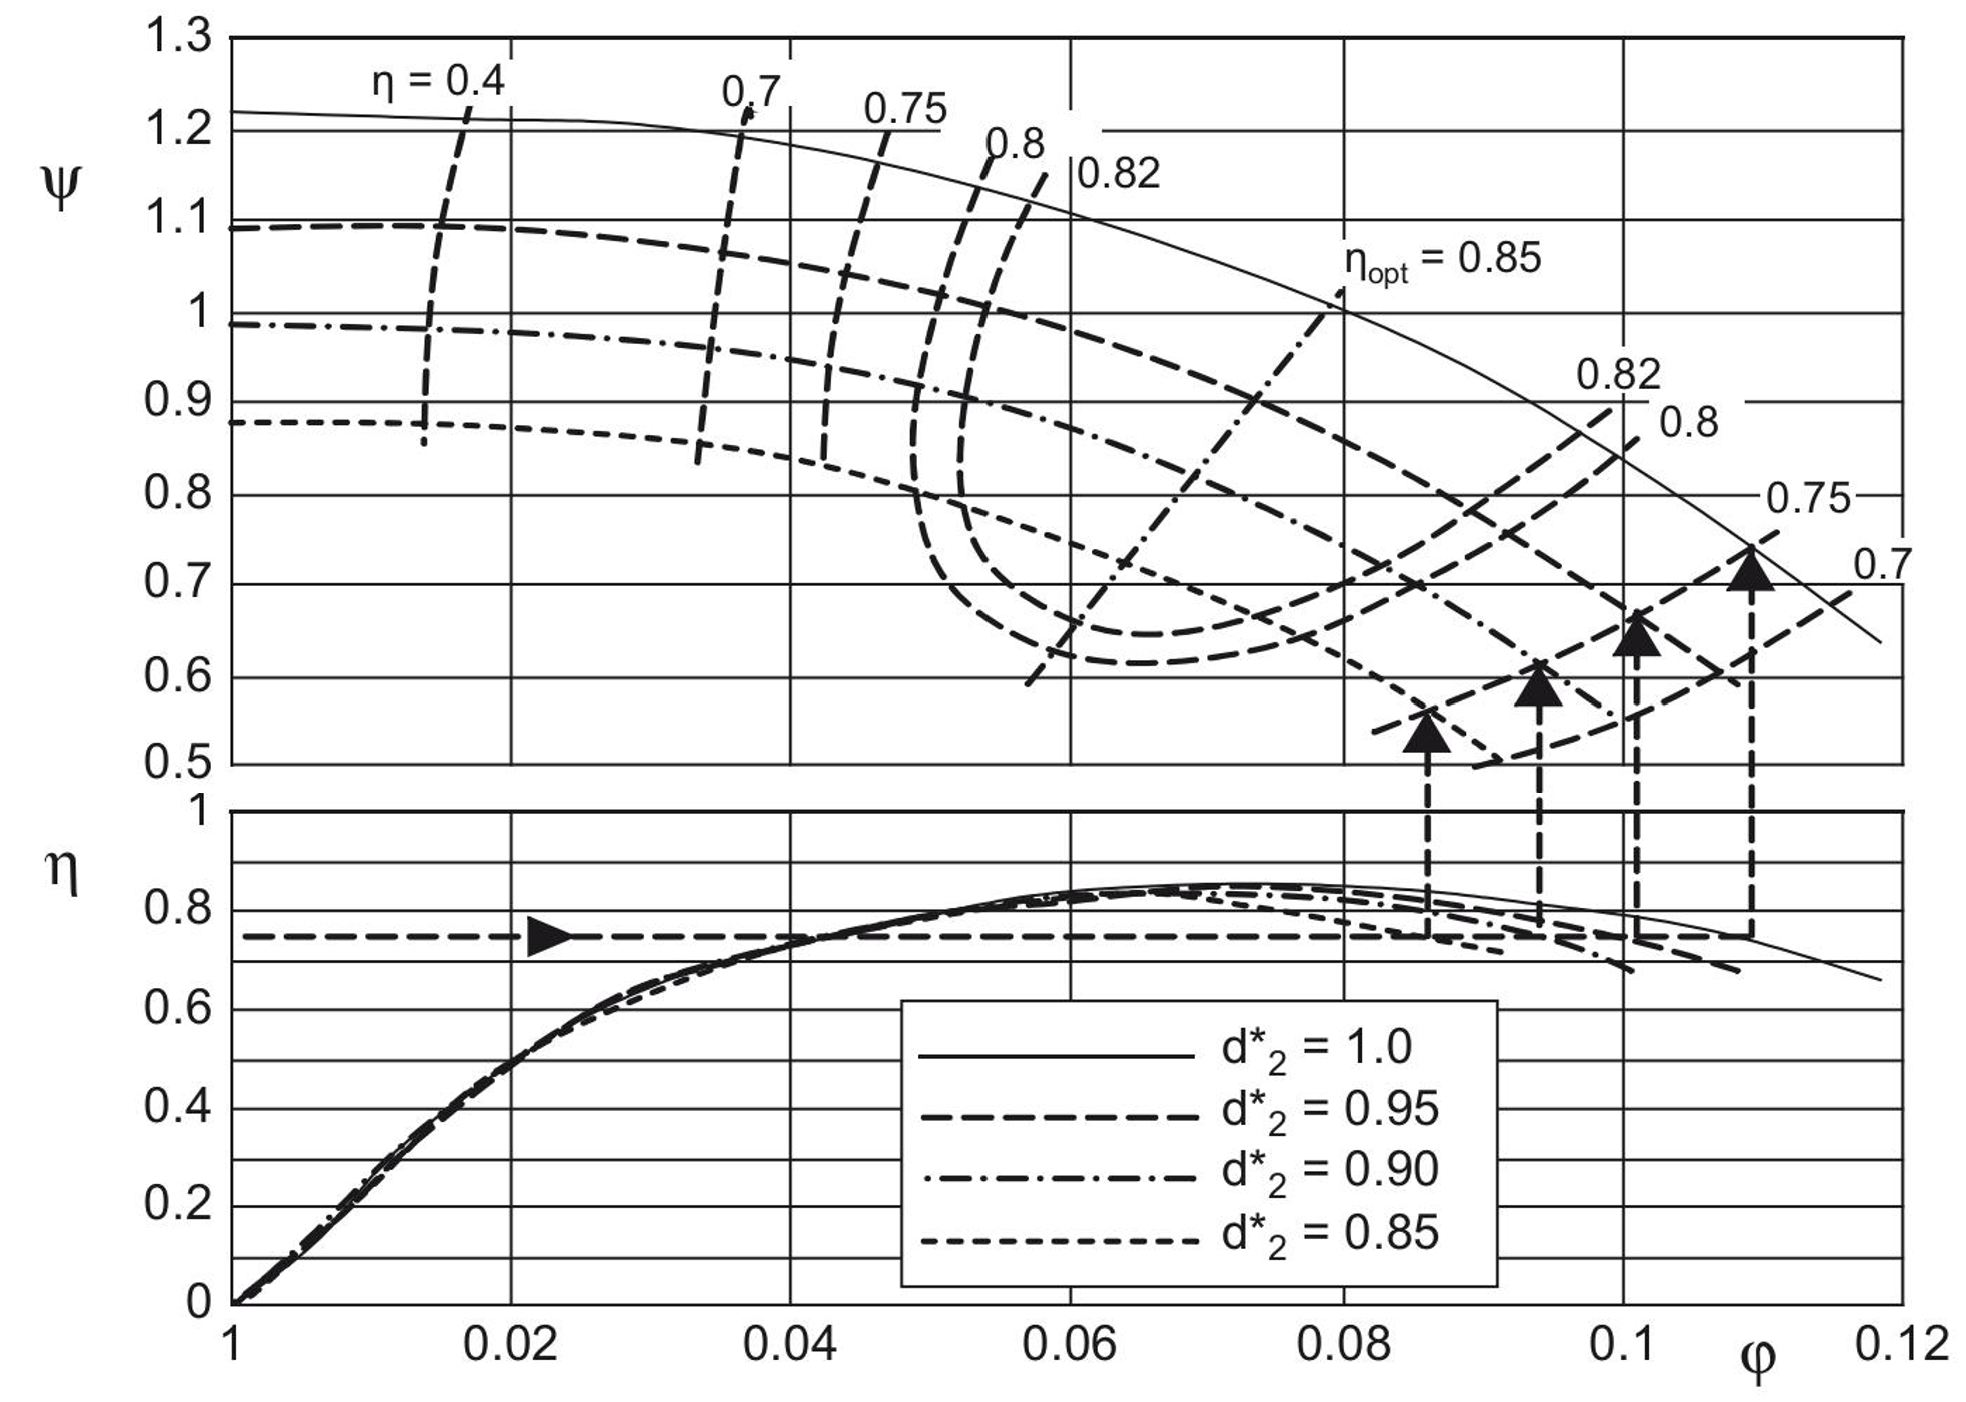
\includegraphics[width=0.8\linewidth]{4_Abbildungen/2_Hauptteil/kreiselpumpe.png}
%  \caption{Kennfeld einer Kreiselpumpe \cite{Gulich.2013}}
%  \label{fig:kreiselpumpe}
%\end{figure}
%\FloatBarrier 

Die Niederdruckpumpen von konventionellen Kraftstoffsystemen erreichen im Reiseflug aufgrund der niedrigeren Drehzahlen und insbesondere Volumenströmen im Vergleich zum optimalen Betriebspunkt nur vergleichsweise niedrige Wirkungsgrade zwischen $53$ und $66\,\%$ \cite{Zhou.2023}. Für die Niederdruckpumpe des Referenzkraftstoffsystems wird ein isentroper Wirkungsgrad von $\eta_{\mathrm{LPFP}}=0,60$ angenommen. Die Niederdruckpumpe des CFM56-5B erzeugt im Auslegungspunkt eine Druckerhöhung von $\Delta p_{\mathrm{MTO}}=$ \SI{965}{\kilo\Pa}. Gemäß den Ähnlichkeitsbeziehungen für Pumpen \cite{Gulich.2013} beträgt der Austrittsdruck $p_{LPFP}$ 

\begin{equation}\label{Eq:lpfp}
	p_{\mathrm{LPFP}}=p_0+\Delta p_{\mathrm{MTO}}\left(\frac{N_2}{N_{2,\mathrm{MTO}}}\right)^2
\end{equation}

der Niederdruckpumpe im Reiseflug somit \SI{930}{\kilo\Pa}.

Da Wasserstoffkraftstoffsysteme keine nennenswerten Kraftstoffmassenströme in die Kraftstofftanks rückführen können, fallen die Volumenströme im Reiseflug relativ zu MTO-Bedingungen nochmals geringer aus als bei konventionellen Kraftstoffsystemen. Brewer \cite{Brewer.1991} berechnet für den Wirkungsgrad einer Hochdruckpumpe mit konstanter Übersetzung im Wasserkraftstoffsystem einen Wert von $\eta_{\mathrm{HPFP}}=0,154$. Mit variabler Übersetzung sind höhere Wirkungsgrade möglich, jedoch verursachte diese Lösung höhere Betriebskosten und wird daher nicht betrachtet \cite{Brewer.1991}. 

\subsection{Zahnradpumpen}

Xu et al. \cite{Xu.2024} haben den Wirkungsgrad einer Zahnrad-Hochdruckpumpe bei unterschiedlichen Drehzahlen untersucht. Hohe Drehzahlen ermöglichen hohe Wirkungsgrade von bis zu $0,78$. Die Hochdruckpumpe des CFM56-5B arbeitet mit einer Nenndrehzahl von $6250$ 1/min \cite{EatonFuelSystemsDivision.2008}. Da die Hochdruckpumpe mit einem konstanten Übersetzungsverhältnis an die Hochdruckwelle angeschlossen ist, beträgt die Drehzahl im Reiseflug (mit $N_2/N_{2,\mathrm{MTO}}=0,88$) $5500$ 1/min. Interpolation der Daten von Xu et al. \cite{Xu.2024} ergibt somit einen Hochdruckpumpenwirkungsgrad von $\eta_{\mathrm{HPFP}}=0,73$.

Für die Hochdruckpumpe wird zudem der geförderte Massenstrom festgelegt. Unter MTO-Bedingungen fördert die Hochdruckpumpe den Kraftstoffverbrauch von \SI{1.054}{\kg\per\s} zuzüglich Kontingenz. Bei einem angenommenen Überschuss von $20\,\%$, beträgt der geförderte Massenstrom bei MTO-Schub \SI{1.265}{\kg\per\s}. Unter Annahme einer identischen volumetrischen Effizienz in beiden Lastpunkten beträgt der geförderte Massenstrom im Reiseflug aufgrund der niedrigeren Drehzahl somit $\dot{m}_\mathrm{HPFP}=$ \SI{1.113}{\kg\per\s}.

\subsection{Wasserstoff-Verdichter}

Aufgrund der geringen Volumenströme bei hohen Druckverhältnissen in Wasserkraftstoffsystemen könnte der Einsatz von Radialverdichtern sinnvoll sein. Der im Reiseflug gegenüber MTO-Bedingungen stark verringerte Volumenstrom bei nur geringfügig verringerter Drehzahl würde bei konstantem Übersetzungsverhältnis eine erhebliche Pumpgefahr bedeuten. Um einen stabilen Betrieb mit hohem Wirkungsgrad zu gewährleisten ist daher eine variable Übersetzung zwischen Verdichter und der Hochdruckwelle des Verdichters notwendig. 

In dieser Arbeit wird für Wasserstoff-Verdichter eine mehrstufige Radialverdichter-Bauweise mit variabler Übersetzung angenommen. Bei einem angenommenen Teillast-Wirkungsgrad des Verdichters von $0,75$ und einem mechanischen Wirkungsgrad der variablen Übersetzung von $0,95$ beträgt der Gesamtwirkungsgrad $\eta_{\mathrm{HPFC}}=\eta_\mathrm{RV}=0,71$.

\section{Wärmeübertrager Druckverluste}

Bei der Auslegung von Wärmeübertragern wird ein Kompromiss zwischen Bauvolumen/Masse und Druckverlust angestrebt. Da Masse und Bauvolumen der Kraftstoffsysteme in dieser Arbeit nicht berücksichtigt werden, erfolgt keine konkrete Auslegung der Wärmeübertrager, etwa mit der NTU-Methode. Stattdessen werden die Druckverluste anhand von Erfahrungswerten abgeschätzt. Für die Wasserstoffkraftstoffsysteme werden die Druckverluste in den Wärmeübertragern mit der parallelen Wasserstoffverbrennung, dem Klimasystem und dem Hauptölsystem sowie des Verdampfer berechnet. Für das Referenzkraftstoffsystem wird ausschließlich der Druckverlust im Wärmeübertrager des Hauptölsystem ermittelt.

\subsection{Referenzkraftstoffsystem}

Zu den kraftstoffseitigen Druckverlusten in Wärmeübertragern konventioneller Kraftstoffsysteme liegen in der Literatur keine zuverlässigen Angaben vor, daher wird der Wert geschätzt. Einerseits sind bei Kerosin-Wärmeübertragern aufgrund der höheren Viskosität von Kerosin im Vergleich zu gasförmigem Wasserstoff sowie der geringeren Temperaturdifferenz der Fluidströme höhere Druckverluste zu erwarten. Andererseits überträgt der FOHE-Wärmeübertrager des konventionellen Kraftstoffsystems aufgrund des höheren Massenstroms eine geringere spezifische Wärme als die der Wasserstoff-Kraftstoffsysteme. Zudem ermöglicht die deutlich höhere Dichte von Kerosin gegenüber gasförmigem Wasserstoff bei konstantem Flächen-zu-Massenstrom-Verhältnis niedrigere Strömungsgeschwindigkeiten, was zu geringeren Druckverluste führt. Unter diesen Abwägungen wird für den FOHE-Wärmeübertrager des Referenzkraftstoffsystems ein Druckverhältnis von $0,95$ angenommen.

\subsection{Wasserstoffkraftstoffsysteme}

Sciatti et al. \cite{Sciatti.2025} haben einen Wärmeübertrager zwischen Wasserstoff und Stickstoff untersucht und ausgelegt. Im Vergleich zum PHC-Wärmeübertrager der Wasserstoff-Kraftstoffsysteme dieser Arbeit sind die Temperaturdifferenz der Fluidströme geringer und die übertragene spezifische Wärme höher. Das von Sciatti et al. ermittelte Druckverhältnis über den Wärmeübertrager von $0,988$ stellt daher eine konservative Abschätzung der Druckverluste des PHC-Wärmeübertragers dar. Jedoch hat der ausgelegte Wärmeübertrager eine für den Wasserstoff-Massenstrom korrigierte Masse von \SI{110.5}{\kg} und ist damit inakzeptabel groß und schwer. Für den PHC-Wärmeübertrager der Wasserstoff-Kraftstoffsysteme wird ein Druckverhältnis von $0,98$ angenommen.

Brewer \cite{Brewer.1991} hat für einen Wasserstoff Wärmeübertrager mit dem Klimasystem Druckverluste von \SI{2.14}{\kilo\Pa} berechnet. Die vernachlässigbar geringen Druckerverluste resultieren aus der geringen übertragenen Wärme bei moderater Temperaturdifferenz.

Brewer \cite{Brewer.1991} hat Wärmeübertrager für ein Wasserstoff-Turbofantriebwerk für Schmalrumpfflugzeuge ausgelegt. Für den Wärmeübertrager mit dem Hauptölsystem hat Brewer ein Druckverhältnis von $0,984$ von berechnet. Die Wärmeübertrager mit den Hauptölsystemen der Wasserstoff-Kraftstoffsysteme dieser Arbeit übertragen das Vierfache der spezifischen Wärme. Die Übertragung der höheren spezifischen Wärme erfordert zusätzliche Rohrreihen im Wärmeübertrager. Da der Druckverlust unterproportional mit der Anzahl an Reihen skaliert \cite{.2013b}, erscheint ein Druckverhältnis über den Wärmeübertrager von $0,95$ realisierbar. Da die Druckverluste des Wärmeübertragers mit dem Klimasystem vernachlässigbar sind, ergibt sich für beide Wärmeübertrager in Summe ein Druckverhältnis von $\pi_{\mathrm{FOHE}}=0,95$.

Sciatti et al. \cite{Sciatti.2025} haben einen Wärmeübertrager für die Verdampfung von Flüssigwasserstoff mit erwärmtem Wasserstoff ausgelegt. Sie haben Druckverluste von \SI{5.74}{\Pa} für die heiße Seite und \SI{10.2}{\Pa} für die kalte Seite berechnet. Die vernachlässigbar geringen Druckverluste resultieren aus der hohen Temperaturdifferenz der Wasserstoff-Massenströme und der vergleichsweise geringen übertragenen Wärme. Für das Wasserstoff-Kraftstoffsystem mit Verdampfer werden daher die Druckverhältnisse $\pi_{\mathrm{V,LP}}=\pi_{\mathrm{V,HP}}=1$ angenommen.

\section{Leitungs- und Injektordruckverluste}

Die Leitungen der Kraftstoffsysteme verursachen Druckverluste infolge von Rohrreibung. Zudem erfordern die Injektoren eine minimale Druckdifferenz zwischen Kraftstoffzufuhr und Brennkammer, um eine adäquate Zerstäubung des Kraftstoffs zu gewährleisten.

\subsection{Referenzkraftstoffsystem}

Die Rohrreibungsverluste im Referenzkraftstoffsystem $\Delta p_\mathrm{L}$ 

\begin{equation}\label{Eq:dp}
	\Delta p_\mathrm{L}=\lambda\frac{L}{D}\frac{\rho}{2}v^2
\end{equation}

werden mit der Darcy-Weisbach-Gleichung bestimmt. Hierbei werden der Rohrreibungswert $\lambda=0,025$, die Leitungslänge $L=$ \SI{0.5}{\m}, der Leitungsdurchmesser $D=$ \SI{14}{\milli\m}, die Kraftstoffdichte $\rho=$ \SI{760}{\kg\per\m\cubed} und die Strömungsgeschwindigkeit $v=$ \SI{10}{\m\per\s} angenommen. Daraus resultiert der Druckverlust $\Delta p_\mathrm{L}=$ \SI{68}{\kilo\Pa}. 

Mazaheri et al. \cite{Mazaheri.2012} haben Drallinjektoren für Luftfahrtanwendungen mit einer Druckdifferenz von $\Delta p_{\mathrm{inj}}=$ \SI{300}{\kilo\Pa} ausgelegt.

\subsection{Wasserstoff-Kraftstoffsysteme}

Die Rohrreibungsverluste der Wasserstoff-Kraftstoffsysteme werden mit der Darcy-Weisbach-Gleichung (Gleichung \ref{Eq:dp}) bestimmt. Hierbei werden der Rohrreibungswert $\lambda=0,02$, die Leitungslänge $L=$ \SI{0.5}{\m}, der Leitungsdurchmesser $D=$ \SI{92}{\milli\m}, die Kraftstoffdichte $\rho=$ \SI{1.33}{\kg\per\m\cubed} und die Strömungsgeschwindigkeit $v=$ \SI{60}{\m\per\s} angenommen. Daraus resultiert der Druckverlust $\Delta p_\mathrm{L}=$ \SI{260}{\kilo\Pa}. 


Brewer \cite{Brewer.1991} hat für ein Wasserkraftstoffsystem Injektor- und Leitungsdruckverluste von $p_{\mathrm{inj}}=$ \SI{168.9}{\kilo\Pa} berechnet.

\section{Parallele Wasserstoffverbrennung}

Zunächst werden die Stoffdaten für das Idealgasmodell bestimmt. Die spezifischen isobaren Wärmekapazitäten der Gase werden jeweils bei der Referenztemperatur $T_{\mathrm{ref}}=$ \SI{298.15}{\K} und Normdruck \SI{101.325}{\kilo\Pa} (bei Wasser beim Dampfdruck) mit dem Webtool für die Eigenschaften von Fluidsystemen des National Institute of Standards and Technology (NIST) bestimmt \cite{NationalInstituteofStandardsandTechnology.2023}. Die molaren Massen der Gase werden mit dem Webtool für chemische Spezies des NIST bestimmt \cite{NationalInstituteofStandardsandTechnology.2}. Der Massenanteil von Sauerstoff wurde ebenfalls der NIST Webseite entnommen \cite{NationalInstituteofStandardsandTechnology.n.d.}. Für Wasserstoff wird ein unterer Heizwert von $H_{u,\mathrm{H}_2}=$ \SI{119960}{\kilo\J\per\kg} angenommen. 

Um hohen Flammentemperaturen entgegenzuwirken, wird ein mageres Kraftstoff-Luft-Äquivalenzverhältnis $\phi_\mathrm{{PHC}}=0,25$ verwendet. Als Kompromiss zwischen Wärmeausbeute und Abmessungen/Gewicht des Wärmeübertragers wird eine minimale Temperaturdifferenz zwischen der Austrittstemperatur der Abgase der parallelen Wasserstoffverbrennung und dem eintretenden kalten Wasserstoffmassenstrom von $\Delta T_{\mathrm{PHC}}=$ \SI{20}{\K} angenommen. 

\section{Korrektur des Kraftstoffmassenstroms}

Die erforderlichen Heizwerte bei den jeweiligen Referenztemperaturen werden aus  GasTurb übernommen \cite{GasTurbGmbH.2021}. Scholz et al. \cite{Scholz.2013} haben einen Wirkungsgrad der Leistungsentnahme der Hochdruckwelle einer modernen Fluggasturbine von $\eta_\mathrm{P}=74\,\%$ berechnet.

\section{Zusammenfassung}

Die Parameter des Referenzkraftstoffsystems sind in Tabelle \ref{Tab:referenz_parametrisiert} gesammelt.

\begin{table}[ht]
    \centering
	\caption{Parametrierung des Referenzkraftstoffsystems}
	\begin{tabular} {|l|c|c|c|c|} \hline%
		\multicolumn{2}{|c|}{Parameter} & Einheit & Wert & Quelle\\ \hline\hline%
        LPFP-Eintrittstemperatur & $T_0$ & K & 270 & - \\ \hline
        LPFP-Eintrittsdruck & $p_0$ & kPa & 180 & \cite{EatonFuelSystemsDivision.2013} \\ \hline
        FOHE-Wärme & $\dot{Q}_{\mathrm{FOHE}}$ & kW & 122 & - \\ \hline
        FOHE-Druckverhältnis & $\pi_{\mathrm{FOHE}}$ & - & 0,95 & - \\ \hline
        IDG-FOHE Wärme  & $\dot{Q}_\mathrm{IDG}$ & kW & 5 & \cite{Sciatti.2024} \\ \hline
        LPFP-Austrittsdruck & $p_\mathrm{LPFP}$ & kPa & 930 & - \\ \hline
        isentroper Wirkungsgrad LPFP & $\eta_\mathrm{LPFP}$ & - & 0,60 & \cite{Zhou.2023} \\ \hline
        isentroper Wirkungsgrad HPFP & $\eta_\mathrm{HPFP}$ & - & 0,73 & \cite{Xu.2024} \\ \hline
        HPFP-Massenstrom & $\dot{m}_\mathrm{HPFP}$ & kg/s & 1,113 & - \\ \hline
        Brennkammer-Massenstrom & $\dot{m}_\mathrm{BK}$ & kg/s & 0,31305 & - \\ \hline
        Leitungs-Druckverluste & $\Delta p_\mathrm{L}$ & kPa & 68 & - \\ \hline
        Injektor-Druckverluste & $\Delta p_\mathrm{inj}$ & kPa & 300 & \cite{Mazaheri.2012} \\ \hline
	\end{tabular}	
    \label{Tab:referenz_parametrisiert}%
\end{table}
\FloatBarrier 

Die Parametrierung der Wasserstoff-Kraftstoffsysteme ist in Tabelle \ref{Tab:h2_parametrisiert} dokumentiert.

\begin{table}[ht]
    \centering
	\caption{Parameter der Modellierungen der Wasserstoff-Kraftstoffsysteme}
	\begin{tabular} {|l|c|c|c|c|} \hline%
    \multicolumn{5}{|c}{Alle Wasserstoff-Kraftstoffsysteme}\\ \hline
    \multicolumn{2}{|c|}{Parameter} & Einheit & Wert & Quelle\\ \hline\hline%
    isentroper Wirkungsgrad RV & $\eta_\mathrm{RV}$ & - & 0,71 & - \\ \hline
    Kraftstoff-Eintrittsdruck & $p_0$ & kPa & 345 & \cite{Brewer.1991, Scholz.2003} \\ \hline
    Kraftstoff-Eintrittstemperatur & $T_0$ & K & 25,2 & \cite{Brewer.1991, Scholz.2003} \\ \hline
    PHCHE-Druckverhältnis  & $\pi_\mathrm{PHC}$ & - & 0,98 & \cite{Sciatti.2025} \\ \hline
    FOHE-Wärme & $\dot{Q}_\mathrm{FOHE}$ & kW & 159 & - \\ \hline
    FOHE-Druckverhältnis & $\pi_\mathrm{FOHE}$ & - & 0,95 & \cite{Brewer.1991} \\ \hline
    Brennkammer-Massenstrom & $\dot{m}_{\mathrm{BK},0}$ & kg/s & 0,10998 & - \\ \hline
    Leitungs-Druckverluste & $\Delta p_\mathrm{L}$ & kPa & 260 & \cite{Brewer.1991} \\ \hline
    Injektor-Druckverluste & $\Delta p_\mathrm{inj}$ & kPa & 168,9 & \cite{Brewer.1991} \\ \hline\hline
	\multicolumn{5}{|c|}{Architektur mit Hochdruckpumpe}\\ \hline
    \multicolumn{2}{|c|}{Parameter} & Einheit & Wert & Quelle\\ \hline\hline%
    isentroper Wirkungsgrad HPFP & $\eta_\mathrm{HPFP}$ & - & 0,154 & \cite{Brewer.1991} \\ \hline
    \multicolumn{5}{|c|}{Architektur mit Verdampfer}\\ \hline
    \multicolumn{2}{|c|}{Parameter} & Einheit & Wert & Quelle\\ \hline\hline%
    isentroper Wirkungsgrad HPFC & $\eta_\mathrm{HPFC}$ & - & 0,71 & - \\ \hline
    Druckverhältnis LP-Verdampfer & $\pi_\mathrm{V,LP}$ & - & 1 & \cite{Sciatti.2025} \\ \hline
    Druckverhältnis HP-Verdampfer & $\pi_\mathrm{V,HP}$ & - & 1 & \cite{Sciatti.2025} \\ \hline\hline
    \multicolumn{5}{|c|}{Architektur mit Vormischung}\\ \hline
    \multicolumn{2}{|c|}{Parameter} & Einheit & Wert & Quelle\\ \hline\hline%
    isentroper Wirkungsgrad HPFC & $\eta_\mathrm{HPFC}$ & - & 0,71 & - \\ \hline
    \end{tabular}	
    \label{Tab:h2_parametrisiert}%
\end{table}
\FloatBarrier 

Für die Modellierung der parallelen Wasserstoffverbrennung sind zusätzlich die in Tabelle \ref{Tab:phc_parametrisiert} geführten Parameter erforderlich.

\begin{table}[ht]
    \centering
	\caption{Parameter der Modellierung der parallelen Wasserstoffverbrennung}
	\begin{tabular} {|l|c|c|c|c|} \hline%
    \multicolumn{2}{|c|}{Parameter} & Einheit & Wert & Quelle\\ \hline\hline%
    isobare Wärmekapazität Sauerstoff & $c_{p, \mathrm{O}_2}$ & \si{\kilo\J\per\kg\per\K} & 0,91963 & \cite{NationalInstituteofStandardsandTechnology.2023} \\ \hline
    isobare Wärmekapazität Stickstoff & $c_{p, \mathrm{N}_2}$ & \si{\kilo\J\per\kg\per\K} & 1,0413 & \cite{NationalInstituteofStandardsandTechnology.2023} \\ \hline
    isobare Wärmekapazität Wasserstoff & $c_{p, \mathrm{H}_2}$ & \si{\kilo\J\per\kg\per\K} & 14,858 & \cite{NationalInstituteofStandardsandTechnology.2023} \\ \hline
    isobare Wärmekapazität Wasser & $c_{p, \mathrm{H}_2\mathrm{O}}$ & \si{\kilo\J\per\kg\per\K} & 1,9118 & \cite{NationalInstituteofStandardsandTechnology.2023} \\ \hline
    molare Masse Sauerstoff & $M_{R, \mathrm{O}_2}$ & g/mol & 31,9988 & \cite{NationalInstituteofStandardsandTechnology.2} \\ \hline
    molare Masse Wasserstoff & $M_{R, \mathrm{H}_2}$ & g/mol & 2,01588 & \cite{NationalInstituteofStandardsandTechnology.2} \\ \hline
    molare Masse Wasser & $M_{R, \mathrm{H}_2\mathrm{O}}$ & g/mol & 18,0153 & \cite{NationalInstituteofStandardsandTechnology.2} \\ \hline
    Äquivalenzverhältnis & $\phi_{\mathrm{PHC}}$ & - & 0,25 & - \\ \hline
    Sauerstoffmassenanteil & $w_{\mathrm{L,O}_2}$ & - & 0,231781 & \cite{NationalInstituteofStandardsandTechnology.n.d.} \\ \hline
    unterer Heizwert Wasserstoff & $H_{u, \mathrm{H}_2}$ & kJ/kg & 119.960 & - \\ \hline
    Referenztemperatur & $T_\mathrm{ref}$ & K & 298,15 & - \\ \hline
    Zapflufttemperatur & $T_\mathrm{Z}$ & K & 272,63 & - \\ \hline
    Umgebungslufttemperatur & $T_\mathrm{U}$ & K & 218,81 & - \\ \hline
    Wirkungsgrad Niederdruckwelle & $\eta_1$ & - & 0,997 & \cite{anonymous.1998} \\ \hline
    Wärmeübertrager Temperaturdifferenz & $\Delta T_\mathrm{PHC}$ & K & 20 & - \\ \hline    
	\end{tabular}	
    \label{Tab:phc_parametrisiert}%
\end{table}
\FloatBarrier 

Die für die Korrektur des Kraftstoffmassenstroms notwendigen Parameter sind in Tabelle \ref{Tab:pot_parametriert} angegeben.

\begin{table}[ht]
    \centering
	\caption{Parameter für die Korrektur des Kraftstoffmassenstroms}
	\begin{tabular} {|l|c|c|c|c|} \hline%
    \multicolumn{2}{|c|}{Parameter} & Einheit & Wert & Quelle\\ \hline\hline%
    unterer Heizwert Wasserstoff & $H_{u, \mathrm{H}_2}$ & kJ/kg & 117.240 & - \\ \hline
    Referenztemperatur H$_2$ & $T_{\mathrm{ref,H}_2}$ & K & 250 & - \\ \hline
    unterer Heizwert Jet-A & $H_{u, \mathrm{Jet-A}}$ & kJ/kg & 42.800 & - \\ \hline
    Referenztemperatur Jet-A & $T_\mathrm{ref,Jet-A}$ & K & 288,15 & - \\ \hline   
    Wirkungsgrad Leistungsentnahme & $\eta_\mathrm{P}$ & - & 0,74 & \cite{Scholz.2013} \\ \hline
	\end{tabular}	
    \label{Tab:pot_parametriert}%
\end{table}
\FloatBarrier 

\section{Brennkammereintrittsbedingungen}

Im Folgenden werden die abhängigen Variablen, also die Brennkammer-Eintrittsbedingungen der Kraftstoffsysteme, erläutert. Zunächst wird der Brennkammer-Eintrittsdruck der Kraftstoffsysteme berechnet. Anschließend wird die zulässige Brennkammer-Eintrittstemperatur für das Referenzkraftstoffsystem bestimmt. Zuletzt werden denkbare Wertebereiche für die Betrachtung der Brennkammer- und Wärmeübertrager-Eintrittstemperaturen der Wasserstoff-Kraftstoffsysteme in einer Parameterstudie bestimmt.

\subsection{Brennkammereintrittsdruck}

Da das Injektordruckverhältnis in der Modellierung berücksichtigt wird, entspricht der erforderliche Brennkammereintrittsdruck des Kraftstoffs, dem Brennkammerdruck im Reiseflug. Der Brennkammer-Eintrittsdruck beträgt somit für alle Kraftstoffsysteme $p_\mathrm{BK}=$ \SI{1330}{\kilo\Pa}.

\subsection{Brennkammer-Eintrittstemperatur Referenzkraftstoffsystem}

Für das Referenzkraftstoffsystem gilt, dass zur Reduzierung der Brennkammer-Eintrittstemperatur eine größere Menge an Kraftstoff in die Kraftstofftanks rückgeführt wird. Um den rückgeführten Kraftstoff zu ersetzen fördert die Niederdruckpumpe einen höheren Kraftstoffmassenstrom, was ihren Leistungsbedarf steigert. Zudem wird aufgrund der geringeren spezifischen Enthalpie ein größerer Kraftstoffmassenstrom benötigt. Aus diesen Gründen wird eine möglichst hohe Brennkammer-Eintrittstemperatur gewählt. 

Der Brennkammer-Eintrittstemperatur ist jedoch durch die maximale Öltemperatur eine technische Obergrenze gesetzt. Der Kraftstoff kann nur bis zu der maximalen Öltemperatur abzüglich der Annäherungstemperatur des Wärmeübertragers erhitzt werden. Bei dem PW1133G Triebwerk beträgt die maximale Öltemperatur im Reiseflug \SI{419.15}{\K} \cite{EASA.2018}. Bei einer angenommenen Annäherungstemperatur zuzüglich Kontingenz von \SI{20}{\K} beträgt die maximal zulässige Brennkammer-Eintrittstemperatur somit $T_\mathrm{BK}=$ \SI{399.15}{\K}.

\subsection{Temperaturen Wasserstoff-Kraftstoffsysteme}

Das EnableH2 Projekt \cite{Patrao.2023} sowie Brewer \cite{Brewer.1991} gehen von Brennkammer-Eintrittstemperaturen von über \SI{650}{\K} aus. Diese hohen Temperaturen erreichen die Autoren insbesondere durch den Einsatz von Wärmerückgewinnung aus dem Abgas des Kerntriebwerks. Die Autoren des CRYOPLANE Berichts \cite{Scholz.2003} und der Joint Cryogenic Engine Study \cite{SIMON.1994} halten Wasserstofftemperaturen von \SI{150}{\K} für ausreichend. Tacconi et al. \cite{Tacconi.2023} haben für ihre Betrachtung eines Wasserstoff-Kraftstoffsystems eine minimale akzeptable Temperatur von \SI{273.15}{\K} angenommen, um Probleme infolge von Vereisung in der Brennkammer zu vermeiden. Aufgrund der breiten Palette an Vorschlägen für Brennkammer-Eintrittstemperaturen für Wasserstoff-Kraftstoffsysteme wird diese Variable in der Parameterstudie in einem Wertebereich zwischen $150$ und \SI{500}{\K} untersucht. Für den Vergleich mit dem Referenzkraftstoffsystem wird ein Wert von \SI{300}{\K} verwendet.

Ähnliches gilt für die Wärmeübertrager-Eintrittstemperatur. Um Vereisungen in den Öl- und Luftwärmeübertragern zu vermeiden, wird eine minimale Eintrittstemperatur gewahrt. Wärmeübertrager-Eintrittstemperaturen oberhalb des Gefrierpunkts von Wasser sind jedoch nicht sinnvoll, da dort keine Vereisungsgefahr mehr besteht und eine weitere Erhöhung der Temperatur lediglich den rezirkulierten Massenstrom erhöhen würde. Der Wärmeübertrager-Eintrittstemperatur ist jedoch durch die Brennkammer-Eintrittstemperatur eine weitere Obergrenze gesetzt. Damit exzessive rezirkulierte Massenströme vermieden werden, wird stets eine Wärmeübertrager-Eintrittstemperatur gewählt, die mindestens \SI{20}{\K} unter der Brennkammer-Eintrittstemperatur liegt. Die Wärmeübertrager-Eintrittstemperatur wird im Rahmen der Parameterstudie in einem Wertebereich zwischen $100$ und \SI{280}{\K} untersucht. Für den Vergleich mit dem Referenzkraftstoffsystem wird ein Wert von \SI{160}{\K} verwendet.

						
%==============================================================================
\chapter{Ergebnisse} \label{chap:ergebnis}
%==============================================================================

In diesem Kapitel werden mit der vorgeschlagenen Modellierung von Kraftstoffsystemen für Fluggasturbinen berechnete Ergebnisse analysiert. Dabei steht insbesondere die Frage im Fokus, ob die Modellierung den Leistungs- und Wärmebedarf der Kraftstoffsysteme akkurat vorhersagen kann. Zunächst wird in einer Sensitivitätsanalyse die Auswirkung von Unsicherheiten der in Kapitel \ref{chap:param} bestimmten Parametern auf das Modellverhalten untersucht. Danach wird die Methodik dieser Arbeit daher mit Daten aus der Literatur validiert. Anschließend wird im Rahmen einer Parameterstudie analysiert, wie sich die Eintrittstemperaturen des Kraftstoffs in den Wärmeübertrager und die Brennkammer auf die Modellierungen der Wasserstoff-Kraftstoffsysteme auswirkt. Abschließend erfolgt ein Vergleich des Betriebsmittelbedarfs der H$_2$-Kraftstoffsysteme untereinander und mit dem Referenzkraftstoffsystem anhand eines ausgewählten Betriebspunkts.

\section{Sensitivitätsanalyse}

Im Folgenden wird eine Sensitivitätsanalyse durchgeführt und ausgewertet, um die für das Modellverhalten maßgeblichen Parameter zu identifizieren. Zunächst werden hierfür die Unsicherheiten der Parameter geschätzt. Anschließend werden die mit Unsicherheit behafteten Parameter in die Modellierungen der Kraftstoffsysteme eingesetzt, um die Abweichungen Leistungsbedarfe zu berechnen.

\subsection{Bestimmung der Schrittweiten}

Da die statistische Verteilung der Parameterwerte nicht bekannt ist, werden die Schrittweiten für die Variation der Parameter geschätzt. Die Schrittweiten werden so gewählt, dass die Abweichung der Pumpenleistung des H$_2$-Kraftstoffsystems mit Verdampfer stets ein positives Vorzeichen aufweist.

Der Austrittsdruck der Niederdruckpumpe $p_\mathrm{LPFP}$ des kerosinbetriebenen Kraftstoffsystems ist stets höher als der Öldruck im Wärmeübertrager des Hauptölsystems und somit von diesem abhängig. Der Öldruck ist eine Funktion der Druckverlust des Ölsystems. Aus diesem Grund wird eine moderate Schrittweite von $-10\,\%$ gewählt.

Da die Druckverluste von Wärmeübertragern und Leitungen ein Auslegungsziel darstellen, sind sie nicht direkt mit Unsicherheit behaftet. Jedoch können abweichende Anforderungen an das Gewicht dieser Komponenten eine Aufweichung der Auslegungsziele erfordern. Um diesen Effekt zu berücksichtigen werden der Leitungsdruckverlust $\Delta p_L$ und die Druckverluste $1-\pi_i$ der Wärmeübertrager mit einer Schrittweite von $+20\,\%$ variiert. 

Die Druckverluste des Verdampfers $1-\pi_{\mathrm{V}, i}$ werden in der Modellierung des Kraftstoffsystems vernachlässigt. Da auf der Hochdruckseite zwar geringe, jedoch im Verhältnis zur Niederdruckseite höhere Druckverluste zu erwarten sind (Siehe Kapitel \ref{chap:param}), werden absolute Schrittweiten von $+0,01$ auf der Hochdruckseite und $+0,005$ auf der Niederdruckseite verwendet. 

Die Unsicherheiten der Wirkungsgrade von Pumpen und Verdichtern $\eta_i$, der verfügbaren Abwärme $\dot{Q}_\mathrm{FOHE}$  und den Injektor-Druckverlusten $\Delta p_\mathrm{inj}$ werden als gering eingeschätzt. Aus diesem Grund wird für diese Parameter eine Schrittweite von $\pm 5\,\%$ ausgewählt.

\subsection{Auswertung der Sensitivitätsanalyse}

Auf Basis der zuvor bestimmten Schrittweiten wird im Folgenden die Sensitivität der Kraftstoffsysteme untersucht und ausgewertet. Zunächst werden die Ergebnisse der Modellierung des H$_2$-Kraftstoffsystems mit Verdampfer präsentiert. Daraufhin werden die Ergebnisse der Sensitivitätsanalysen der H$_2$-Kraftstoffsysteme miteinander verglichen. Abschließend werden die Ergebnisse der Sensitivitätsanalyse für das kerosinbetriebene Kraftstoffsystem diskutiert.

Die Ergebnisse der Sensitivitätsanalyse für das H$_2$-Kraftstoffsystem mit Verdampfer sind in Tabelle \ref{Tab:sensjeta} dargestellt.

\begin{table}[ht]
	\centering
	\caption{Sensitivitätsanalyse des H$_2$-Kraftstoffsystems mit Verdampfer}
	\begin{tabular} {|l|c|c|c|c|c|} \hline%
		Parameter & Einheit & Schrittweite & Schrittweite [\%] & $ \Delta \sum P_i$ [\%] \\ \hline\hline%
		$\Delta p_\mathrm{L}$ & \si{\kilo\Pa} & +52,0 & +20,0 & +5,39 \\ \hline 
		$1-\pi_\mathrm{FOHE}$ & - & +0,010 & +20,0 & +1,98 \\ \hline 
		$1-\pi_\mathrm{PHC}$ & - & +0,004 & +20,0 & +0,768 \\ \hline
		$\eta_\mathrm{HPFC}$ & - & -0,0355 & -5,00 & +2,68 \\ \hline  
		$\eta_\mathrm{RV}$ & - & -0,0355 & -5,00 & +1,71 \\ \hline 
		$\dot{Q}_\mathrm{FOHE}$ & \si{\kilo\W} & -7,95 & -5,00 & +0,0541 \\ \hline 
		$\Delta p_\mathrm{inj}$ & \si{\kilo\Pa} & +8,45 & +5,00 & +0,0829 \\ \hline 
		$1-\pi_\mathrm{V, HP}$ & - & +0,010 & - & +1,88 \\ \hline 
		$1-\pi_\mathrm{V, LP}$ & - & +0,005 & - & +0,202 \\ \hline 
	\end{tabular}	
	\label{Tab:sensafter}%
\end{table}
\FloatBarrier 

Mit einem Anstieg der Leistungen um  $+5,39\,\%$ hat die Erhöhung der Leitungs-Druckverluste bei Weitem die größte Auswirkung auf die Modellierung des H$_2$-Kraftstoffsystems mit Verdampfer. Die Reduktionen der Wirkungsgrade der Verdichter haben mit $+2,68\,\%$ (Hochdruckverdichter) beziehungsweise $+1,71\,\%$ (Rezirkulationsverdichter) nur eine moderate Auswirkung auf die Verdichterleistungen. 

Die Erhöhungen der Druckverluste des Ölsystem-Wärmeübertragers und der Hochdruckseite des Verdampfers führen mit $1,98\,\%$ und $1,88\,\%$ ebenfalls zu moderaten anstiegen der Leistungen. Hingegen hat der Anstieg der Druckverluste des PHC-Wärmeübertragers und der Niederdruckseite des Verdampfers nur geringen Einfluss auf die Leistungen. 

Ein Anstieg der Injektor-Druckverluste hat nur geringe Auswirkungen auf die Verdichter-Leistungen.


Die Tabellen \ref{Tab:senspump} und \ref{Tab:sensdual} zeigen die Ergebnisse der Sensitivitätsanalysen für die H$_2$-Kraftstoffsysteme mit Hochdruckpumpe und Vormischung.

\begin{table}[ht]
	\centering
	\caption{Sensitivitätsanalyse des H$_2$-Kraftstoffsystems mit Pumpe}
	\begin{tabular} {|l|c|c|c|c|c|} \hline%
		Parameter & Einheit & Schrittweite & Schrittweite [\%] & $ \Delta \sum P_i$ [\%] \\ \hline\hline%
		$\Delta p_\mathrm{L}$ & \si{\kilo\Pa} & +52,0 & +20,0 & +8,19 \\ \hline 
		$1-\pi_\mathrm{FOHE}$ & - & +0,010 & +20,0 & +3,01 \\ \hline 
		$1-\pi_\mathrm{PHC}$ & - & +0,004 & +20,0 & +1,17 \\ \hline
		$\eta_\mathrm{HPFP}$ & - & -0,0077 & -5,00 & +1,41 \\ \hline  
		$\eta_\mathrm{RV}$ & - & -0,0355 & -5,00 & +2,96 \\ \hline 
		$\dot{Q}_\mathrm{FOHE}$ & \si{\kilo\W} & -7,95 & -5,00 & +0,055 \\ \hline 
		$\Delta p_\mathrm{inj}$ & \si{\kilo\Pa} & +8,45 & +5,00 & -0,0523 \\ \hline 
	\end{tabular}	
	\label{Tab:senspump}%
\end{table}
\FloatBarrier 

\begin{table}[ht]
	\centering
	\caption{Sensitivitätsanalyse des H$_2$-Kraftstoffsystems mit Vormischung}
	\begin{tabular} {|l|c|c|c|c|c|} \hline%
		Parameter & Einheit & Schrittweite & Schrittweite [\%] & $ \Delta \sum P_i$ [\%] \\ \hline\hline%
		$\Delta p_\mathrm{L}$ & \si{\kilo\Pa} & +52,0 & +20,0 & +5,38 \\ \hline 
		$1-\pi_\mathrm{FOHE}$ & - & +0,010 & +20,0 & +1,97 \\ \hline 
		$1-\pi_\mathrm{PHC}$ & - & +0,004 & +20,0 & +0,766 \\ \hline
		$\eta_\mathrm{HPFC}$ & - & -0,0355 & -5,00 & +2,68 \\ \hline  
		$\eta_\mathrm{RV}$ & - & -0,0355 & -5,00 & +1,70 \\ \hline 
		$\dot{Q}_\mathrm{FOHE}$ & \si{\kilo\W} & -7,95 & -5,00 & +0,0551 \\ \hline 
		$\Delta p_\mathrm{inj}$ & \si{\kilo\Pa} & +8,45 & +5,00 & +0,0838 \\ \hline 
	\end{tabular}	
	\label{Tab:sensdual}%
\end{table}
\FloatBarrier 

Die H$_2$-Kraftstoffsysteme weisen nur geringfügige Unterschiede in ihren Sensitivitäten auf. Das H$_2$-Kraftstoffsystem mit Hochdruckpumpe zeigt mit $+8,19\,\%$ eine besonders hohe Sensitivität gegenüber Variationen der Leitungs-Druckverluste. Auch Änderungen der Druckverluste in den Wärmeübertragern haben einen stärkeren Einfluss auf dieses System. Die Ergebnisse des H$_2$-Kraftstoffsystems mit Vormischung weichen nur minimal von denen des H$_2$-Kraftstoffsystems mit Verdampfer ab.

Die Ergebnisse der Sensitivitätsanalyse für das kerosinbetriebene Kraftstoffsystem sind in Tabelle \ref{Tab:sensjeta} zusammengefasst.

\begin{table}[ht]
	\centering
	\caption{Sensitivitätsanalyse des kerosinbetriebenen Kraftstoffsystems}
	\begin{tabular} {|l|c|c|c|c|} \hline%
		Parameter & Einheit & Schrittweite & Schrittweite [\%] & $ \Delta \sum P_i$ [\%] \\ \hline\hline%
		$p_\mathrm{LPFP}$ & - & -93,0 & -10,0 & +4,38 \\ \hline 
		$\Delta p_\mathrm{L}$ & \si{\kilo\Pa} & +13,6 & +20,0 & +1,21 \\ \hline 
		$1-\pi_\mathrm{FOHE}$ & - & +0,010 & +20,0 & +0,828 \\ \hline 
		$\eta_\mathrm{HPFP}$ & - & -0,0365 & -5,00 & +3,81 \\ \hline 
		$\eta_\mathrm{LPFP}$ & - & -0,030 & -5,00 & +1,48 \\ \hline 
		$\dot{Q}_\mathrm{FOHE}$ & \si{\kilo\W} & -6,35 & -5,20 & -1,36 \\ \hline 
		$\Delta p_\mathrm{inj}$ & \si{\kilo\Pa} & +30,0 & +10,0 & +2,67 \\ \hline 
	\end{tabular}	
	\label{Tab:sensjeta}%
\end{table}
\FloatBarrier 

Zwar führt der verringerte Austrittsdruck zu einer geringeren Leistung der Niederdruckpumpe, jedoch steigt hierdurch das Druckverhältnis und die Leistung der Hochdruckpumpe. Die Auswirkungen auf die Hochdruckpumpe überwiegen, was zu einem Anstieg des Leistungsbedarfs um $4,38\,\%$ führt – der größten Abweichung unter den Parametern. 

Eine Verringerung des Wirkungsgrads der Hochdruckpumpe hat einen um $3,81\,\%$ höheren Leistungsbedarf zur Folge. Aufgrund des geringeren Leistungsbedarfs der Niederdruckpumpe hat die Variation ihres Wirkungsgrads mit $1,48\,\%$ eine geringere Auswirkung. 

Eine Steigerung der Injektor-Druckverluste führt zu einem um $2,67\,\%$ höheren Leistungsbedarf der Pumpen. Im Vergleich haben die Variation der Leitungs- und Wärmeübertrager-Druckverluste einen geringen Einfluss auf den Leistungsbedarf. 

Die kleinere Abwärme führt zu einem geringeren Massenstrom durch die Niederdruckpumpe und somit zu einer um $1,36\,\%$ verringerten Pumpenleistung.

\section{Validierung}

Zur Validierung der Methodik dieser Arbeit wird das Wasserstoff-Kraftstoffsystem mit Pumpe angepasst und parametriert, um das von Brewer \cite{Brewer.1991} vorgeschlagene Kraftstoffsystem nachzuempfinden. 

Dabei werden folgende Modifikationen an der Modellierung vorgenommen: Die Druckverluste im rezirkulierten Kraftstoffstrom werden vernachlässigt, da das Kraftstoffsystem nach Brewer keinen Rezirkulationsverdichter vorsieht. Der Kraftstoffmassenstrom wird nicht an die Brennkammer-Eintrittstemperatur angepasst und eine parallele Wasserstoffverbrennung ist nicht vorgesehen. Zudem bleibt der Wärmeeintrag des von Brewer vorgeschlagenen Rekuperators unberücksichtigt, da sich dieser Wärmeübertrager Stromabwärts der Entnahmestelle des rezirkulierten Kraftstoffs befindet - eine Konfiguration, die von der Modellierung dieser Arbeit abweicht. Um dennoch eine Vergleichbarkeit der Pumpenleistung zu gewährleisten, wird der Druckverlust dieses Wärmeübertragers zu den Druckverluste der Injektoren addiert. 

Ein weiterer Unterschied liegt in der Modellierung des Kraftstoffs: Während in dieser Arbeit Parawasserstoff verwendet wird, basieren Brewers Berechnungen auf Normalwasserstoff. Dies macht eine Anpassung der Modellparameter des Wasserstoff-Stoffmodels erforderlich. Tabelle \ref{Tab:brewer} zeigt die weiteren Änderungen der Parameter und Variablen gegenüber dem ursprünglichen Wasserstoff-Kraftstoffsystem mit Pumpe.

\begin{table}[ht]
    \centering
	\caption{Veränderte Parameter der Validierung}
	\begin{tabular} {|l|c|c|c|} \hline%
    \multicolumn{2}{|c|}{Parameter} & Einheit & Wert\\ \hline\hline%
    FOHE Druckverhältnis & $\pi_\mathrm{FOHE}$ & - & 1 \\ \hline
    Brennkammer-Massenstrom & $\dot{m}_\mathrm{BK}$ & kg/s & 0,166 \\ \hline
    Leitungsdruckverluste & $\Delta p_\mathrm{r}$ & kPa & 30 \\ \hline
    Injektordruckverluste & $\Delta p_\mathrm{inj}$ & kPa & 214,4 \\ \hline
    Brennkammer-Eintrittsdruck & $p_\mathrm{BK}$ & kPa & 1516,2 \\ \hline
    Brennkammer-Eintrittstemperatur & $T_\mathrm{BK}$ & K & 264 \\ \hline
    Wärmeübertrager-Eintrittstemperatur & $T_\mathrm{W}$ & K & 200 \\ \hline
    \end{tabular}	
    \label{Tab:brewer}%
\end{table}
\FloatBarrier 

Tabelle \ref{Tab:validation} zeigt die von Brewer berechneten Werte und die mit der beschriebenen Methodik berechneten Werte. 

\begin{table}[ht]
    \centering
	\caption{Validierung der Methodik}
	\begin{tabular} {|l|c|c|c|c|} \hline%
    \multicolumn{2}{|c|}{Variable} & Einheit & Brewer \cite{Brewer.1991} & Diese Arbeit \\ \hline\hline%
    Pumpenleistung & $P_\mathrm{HPFP}$ & kW & 23,9 & 23,4 \\ \hline
    Wärme & $\dot{Q}$ & kW & 542,7 & 539,8 \\ \hline
    Rezirkulierter Massenstrom & $\dot{m}_\mathrm{R}$ & kg/s & 0,377 & 0,439 \\ \hline
    Pumpen-Austrittstemperatur & $T_{2,\mathrm{HPFP}}$ & K & 50 & 33,1 \\ \hline
    \end{tabular}	
    \label{Tab:validation}%
\end{table}
\FloatBarrier 

Die Werte für die Pumpenleistung und den Wärmebedarf stimmen weitgehend mit den Berechnungen von Brewer überein. Allerdings berechnet Brewers einen um $14\,\%$ geringeren rezirkulierten Massenstrom, was auf die um \SI{16.9}{\K} höhere Pumpen-Austrittstemperatur mit seinem Modell zurückzuführen ist. Um den Ursprung dieser Abweichung zu identifizieren, wird die Energiebilanz verwendet. Die Energiebilanz um die Hochdruckpumpe des Brewer-Konzepts 

\begin{equation}\label{Eq:brewer}
	\Delta \dot{E}_\mathrm{HPFP}=\dot{m}_\mathrm{BK}(h(T_0,p_0)-h(T_\mathrm{HPFP}, p_\mathrm{HPFP}))+P_\mathrm{HPFP}
\end{equation}

weist ein Residuum von $\Delta \dot{E}_\mathrm{HPFP}=$ \SI{-79.9}{\kilo\W} auf. Ähnliche Energiebilanzen für die Wasserstoffmischung und die Wärmeübertrager ergeben Residuen von $\Delta \dot{E}_\mathrm{mix}=$ \SI{25.3}{\kilo\W} und $\Delta \dot{E}_\mathrm{W}=$ \SI{57.2}{\kilo\W}. Da das Residuum der Energiebilanz des gesamten Kraftstoffsystems mit $\Delta \dot{E}=$ \SI{2.3}{\kilo\W} gering ist, erscheint ein Fehlerursprung im verwendeten Stoffmodell als unwahrscheinlich. Die Abweichungen auf Komponenten-Ebene könnten durch einen nicht dokumentierten Wärmeübertrager zwischen flüssigem und verdampften Wasserstoff erklärt werden. Aufgrund dieser Problematik ist eine belastbare Validierung der Methodik dieser Arbeit nicht möglich.

\section{Parameterstudie}

Um die Wechselwirkung zwischen Wärmeübertrager- und Brennkammer-Eintrittstemperatur auf die Betriebsmittelbedarfe der Wasserstoff-Kraftstoffsysteme zu untersuchen wird eine zweidimensionale Parameterstudie durchgeführt. Die Parameter und Konfiguration der Wasserstoff-Kraftstoffsysteme werden über den untersuchten Bereich als konstant angenommen. Da sich die Wasserstoff-Kraftstoffsysteme untereinander in ihrem Verhalten weitgehend ähneln, werden die Ergebnisse zunächst für die Architektur mit Hochdruckpumpe gezeigt. Anschließend werden die Unterschiede zwischen den Architekturen im Detail betrachtet.

\subsection{Architektur mit Hochdruckpumpe}

Abbildung \ref{fig:pumppower} zeigt den mechanischen Leistungsbedarf des Wasserstoff-Kraftstoffsystems mit Pumpe für den untersuchten Temperaturbereich. 

\begin{figure}[ht]
\centering
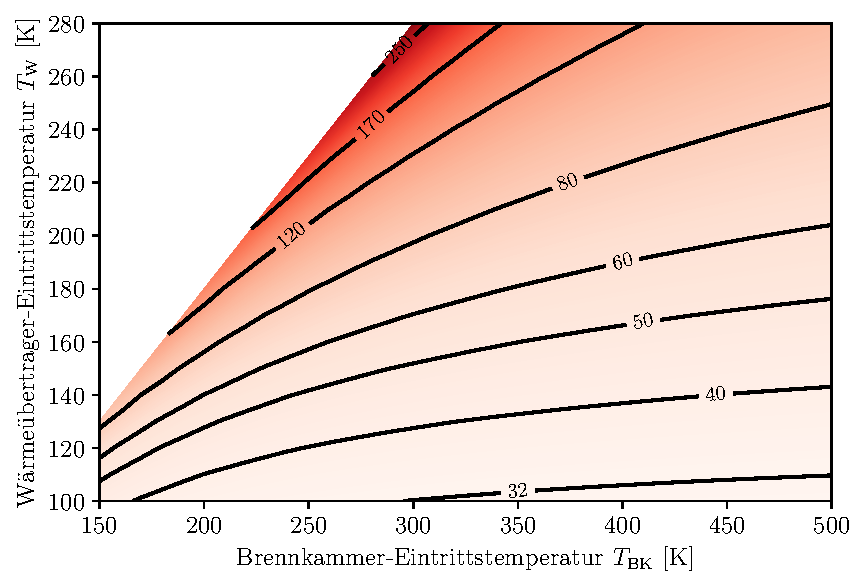
\includegraphics[width=0.9\linewidth]{4_Abbildungen/2_Hauptteil/Ergebnisse/Pumpepowercontour.pdf}
  \caption{Leistungsbedarf Wasserstoff-Kraftstoffsystem mit Pumpe [kW]}
  \label{fig:pumppower}
\end{figure}
\FloatBarrier

Der Gesamtleistungsbedarf steigt mit zunehmender Wärmeübertrager-Eintrittstemperatur, da die geringe Differenz zur Brennkammer-Eintrittstemperatur einen größeren Rezirkulations-Massenstrom erfordert, was die Leistung des Rezirkulationsverdichters erhöht. Zwar führen höhere Brennkammer-Eintrittstemperaturen zu einer Zunahme der spezifischen Arbeit des Rezirkulationsverdichters, jedoch wird dieser Effekt durch den aufgrund der erhöhten Temperaturdifferenz reduzierten rezirkulierten Massenstrom mehr als ausgeglichen. Die Leistung der Hochdruckpumpe ist hingegen unabhängig von den Eintrittstemperaturen (Abbildung \ref{fig:pumpsplit}). 

\begin{figure}[ht]
\centering
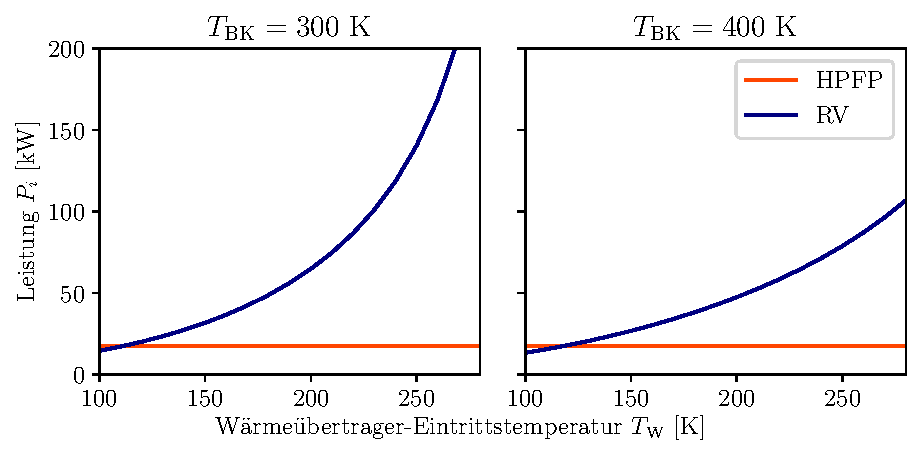
\includegraphics[width=0.9\linewidth]{4_Abbildungen/2_Hauptteil/Ergebnisse/Pumpe_powersplit.pdf}
  \caption{Leistungsaufteilung Architektur mit Pumpe}
  \label{fig:pumpsplit}
\end{figure}
\FloatBarrier

Der Wärmebedarf ist insbesondere mit der Brennkammer-Eintrittstemperatur korreliert. Da die Leistung des Rezirkulationsverdichters mit steigender Wärmeübertrager-Eintrittstemperatur beziehungsweise geringer Differenz der Eintrittstemperaturen zunimmt, liegt in diesem Fall ein verringerter Wärmebedarf vor. Dieses Verhalten ist in Abbildung \ref{fig:pumpheat} dargestellt.

\begin{figure}[ht]
\centering
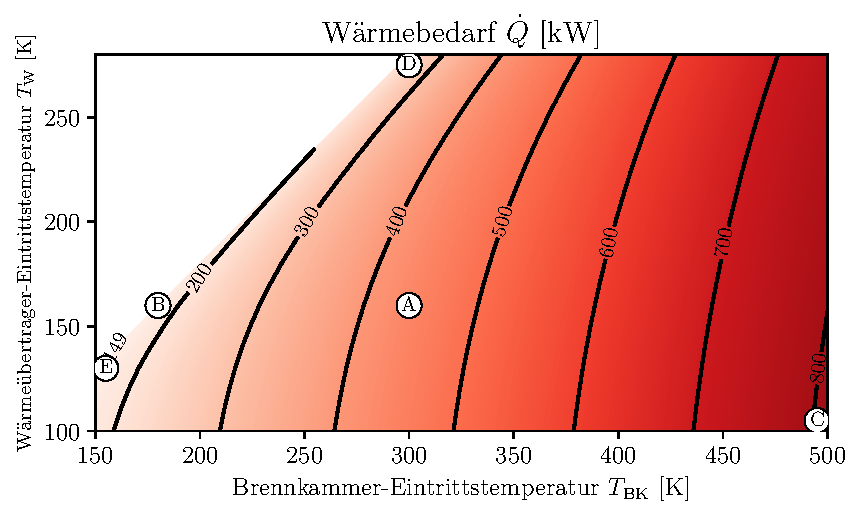
\includegraphics[width=0.9\linewidth]{4_Abbildungen/2_Hauptteil/Ergebnisse/Pumpeheatcontour.pdf}
  \caption{Wärmebedarf Wasserstoff-Kraftstoffsystem mit Pumpe [kW]}
  \label{fig:pumpheat}
\end{figure}
\FloatBarrier

Abbildung \ref{fig:pumpfuel} zeigt den Kraftstoffverbrauch des Triebwerks mit dem Kraftstoffsystem mit Pumpe für die unterschiedlichen Eintrittstemperaturen.

\begin{figure}[ht]
\centering
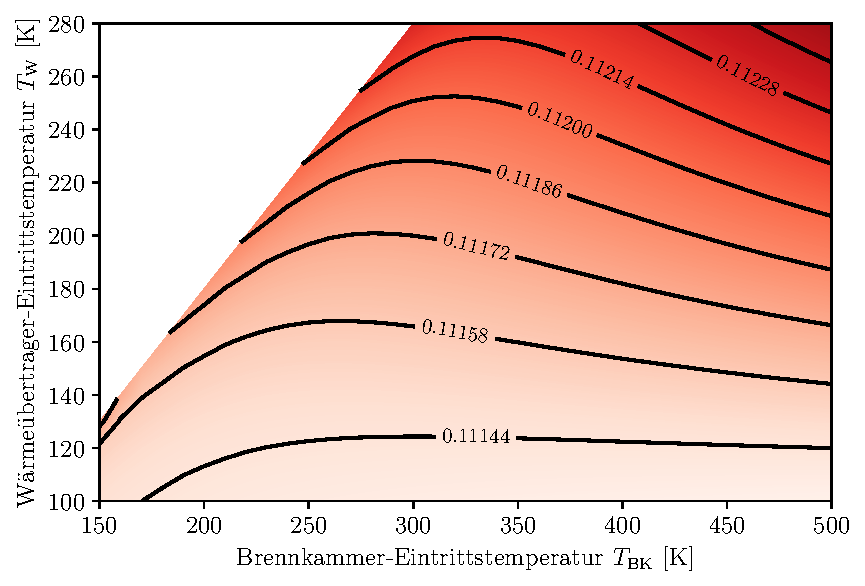
\includegraphics[width=0.9\linewidth]{4_Abbildungen/2_Hauptteil/Ergebnisse/Pumpemassflowcontour.pdf}
  \caption{Kraftstoffverbrauch Wasserstoff-Kraftstoffsystem mit Pumpe [kg/s]}
  \label{fig:pumpfuel}
\end{figure}
\FloatBarrier

Die Leistung des Rezirkulationsverdichters bei hohen Wärmeübertrager-Eintritts-temperaturen verringert den Gesamtwirkungsgrad des Triebwerks. Im Gegensatz dazu hat die Brennkammer-Eintrittstemperatur einen geringeren Einfluss auf den Verbrauch.


\subsection{Vergleich der Wasserstoff-Kraftstoffsysteme}

Im Folgenden werden die Ergebnisse der Parameterstudie für die verschiedenen Wasserstoff-Kraftstoffsysteme miteinander verglichen. Abbildung \ref{fig:comp_power} zeigt den Leistungsbedarf der Kraftstoffsysteme in Abhängigkeit der Wärmeübertrager-Eintrittstemperatur für zwei verschiedene Brennkammer-Eintrittstemperaturen.

\begin{figure}[ht]
\centering
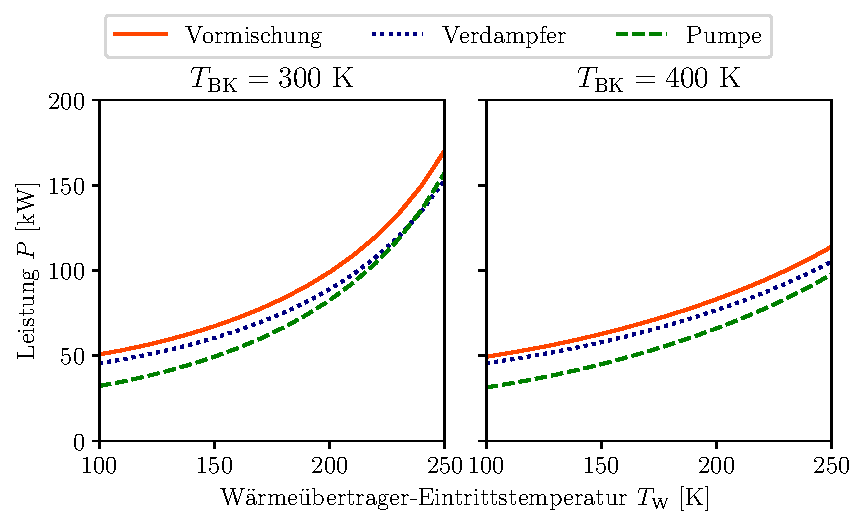
\includegraphics[width=0.9\linewidth]{4_Abbildungen/2_Hauptteil/Ergebnisse/summary_power.pdf}
  \caption{Leistungsbedarf Wasserstoff-Kraftstoffsysteme}
  \label{fig:comp_power}
\end{figure}
\FloatBarrier

Aufgrund der höheren spezifischen Arbeit der Verdichtung im gasförmigen Zustand weisen beide Verdichterarchitekturen im Vergleich zur Pumpenarchitektur einen erhöhten Leistungsbedarf auf. Da die Verdichter des Kraftstoffsystems mit Vormischung bei identischer spezifischer Arbeit einen größeren Massenstrom  fördern als die Verdichter der Architektur mit Verdampfer, hat das Kraftstoffsystem mit Vormischung einen höheren Leistungsbedarf. Dieser Effekt wird bei höheren Brennkammer-Eintrittstemperaturen abgeschwächt, da die Verdampfung in diesem Fall einen geringeren Massenstrom erfordert. Abbildung \ref{fig:comp_split} zeigt den Einfluss der Wärmeübertrager-Eintrittstemperatur auf die Komponenten-Leistungen.

\begin{figure}[ht]
\centering
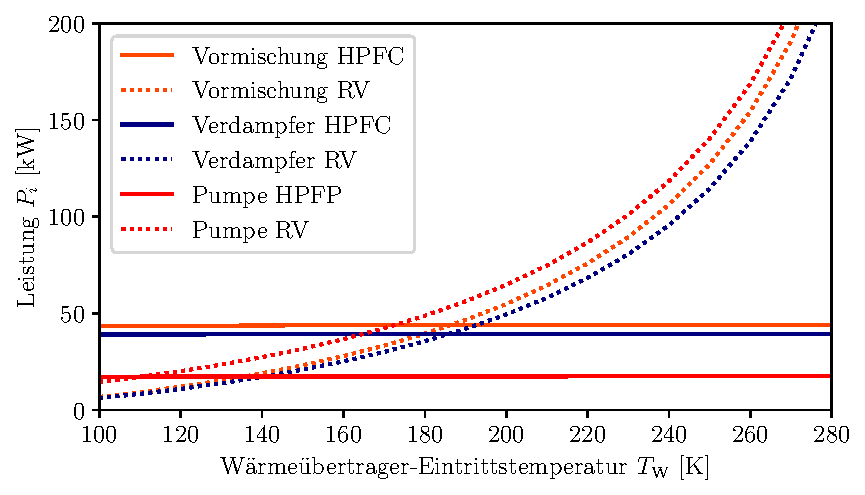
\includegraphics[width=0.9\linewidth]{4_Abbildungen/2_Hauptteil/Ergebnisse/300summary_powersplit.pdf}
  \caption{Leistungsaufteilung Vergleich [$T_\mathrm{BK}=$ \SI{300}{\K}]}
  \label{fig:comp_split}
\end{figure}
\FloatBarrier

Analog zur Architektur mit Pumpe hat die Wärmeübertrager-Eintrittstemperatur bei den Verdichterarchitekturen keinen Einfluss auf die Leistung des Hochdruckverdichters. Da die Verdichterarchitekturen im Vergleich zur Pumpenarchitektur einen geringeren Rezirkulationsmassenstrom aufweisen, fällt auch die Leistung des Rezirkulationsverdichters geringer aus. Abbildung \ref{fig:tbk_split} zeigt den Einfluss der Brennkammer-Eintrittstemperatur auf die Komponenten-Leistungen.

\begin{figure}[ht]
\centering
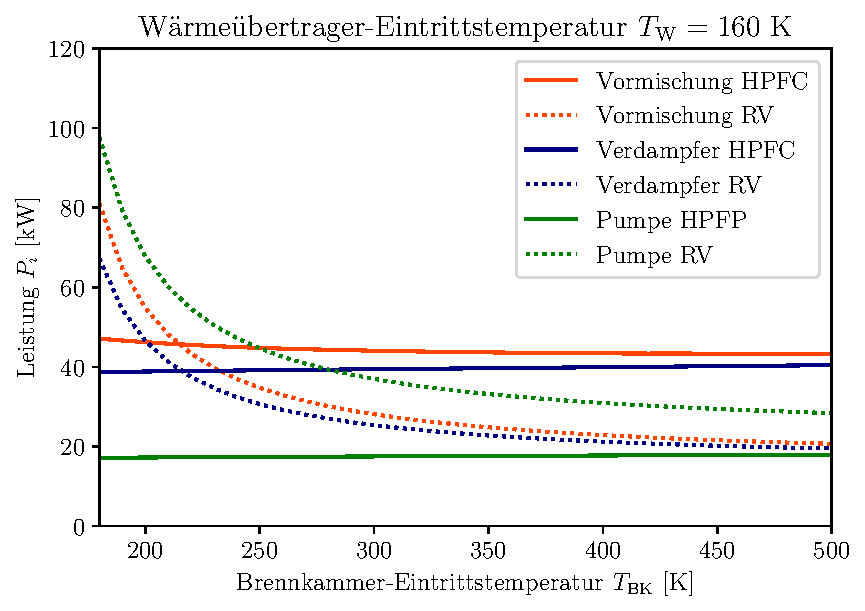
\includegraphics[width=0.7\linewidth]{4_Abbildungen/2_Hauptteil/Ergebnisse/tbkcomp.pdf}
  \caption{Leistungsaufteilung Vergleich [$T_\mathrm{W}=$ \SI{160}{\K}]}
  \label{fig:tbk_split}
\end{figure}
\FloatBarrier

Der Trend sinkender Leistung des Rezirkulationsverdichters bei höherer Differenz der Eintrittstemperaturen setzt sich auch bei den Verdichterarchitekturen fort. Im Gegensatz zu den anderen Architekturen führen steigende Brennkammer-Eintrittstemperaturen bei der Architektur mit Vormischung jedoch zu einer geringfügigen Reduzierung der Leistung des Hochdruckverdichters. Dies ist auf den geringeren erforderlichen Massenstrom für die Verdampfung zurückzuführen. 

Abbildung \ref{fig:stackplot} gibt einen Überblick der Leistungsanteile der Wasserstoff-Kraftstoffsysteme. In der linken Spalte sind die Leistungsanteile in Abhängigkeit der Brennkammereintritts-Temperatur bei konstanter Wärmeübertrager-Eintrittstemperatur dargestellt. Die mittlere Spalte zeigt die Leistungsanteile in Abhängigkeit der Brennkammer-Eintrittstemperatur, aber mit konstanter Temperaturdifferenz. Die rechte Spalte zeigt die Leistungsanteile in Abhängigkeit der Wärmeübertrager-Temperatur bei konstanter Brennkammereintritts-Eintrittstemperatur.

\begin{figure}[ht]
\centering
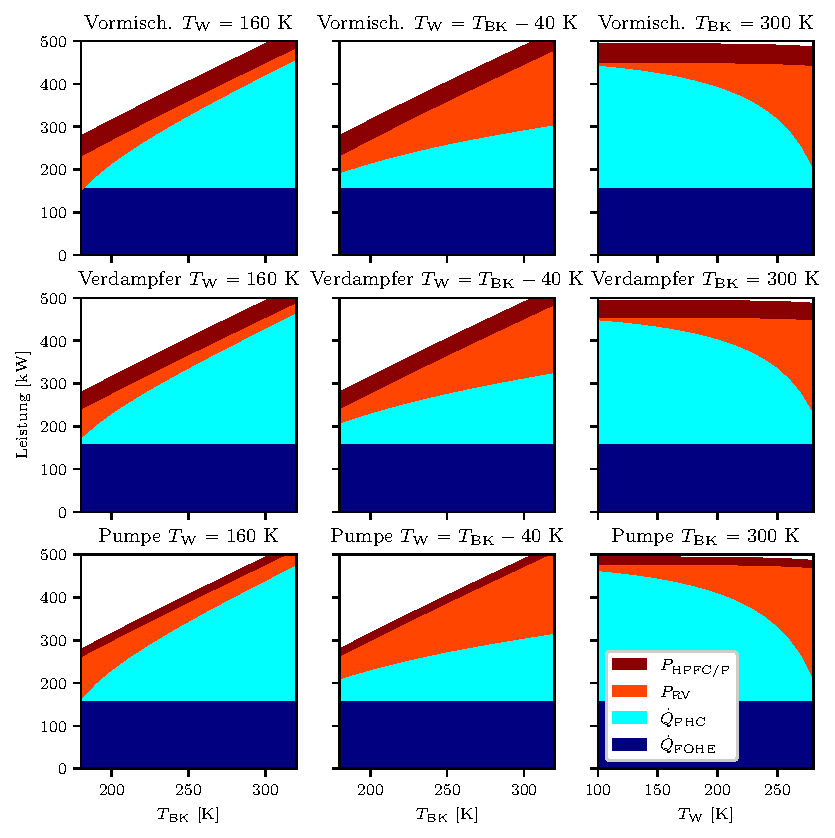
\includegraphics[width=1\linewidth]{4_Abbildungen/2_Hauptteil/Ergebnisse/stackplot_summary.pdf}
  \caption{Stapeldiagramme der Leistungsanteile}
  \label{fig:stackplot}
\end{figure}
\FloatBarrier

Diese Abbildung verdeutlicht den Einfluss der Differenz der Eintrittstemperaturen. Bei einer konstanten Temperaturdifferenz von $T_{BK}-T_W=$ \SI{40}{\K} (mittlere Spalte) liegen die Leistung des Rezirkulationsverdichters $P_{RV}$ und die Wärme der parallelen Wasserstoffverbrennung $\dot{Q}_{PHC}$ über die untersuchten Brennkammer-Eintrittstemperaturen betragsmäßig in einem ähnlichen Bereich. Im Gegensatz dazu nimmt bei konstanter Brennkammer-Eintrittstemperatur der Leistungsanteil des Rezirkulationsverdichters mit steigender Wärmeübertrager-Eintrittstemperatur zu (rechte Spalte).

Eine direkte Empfehlung spezifischer Eintrittstemperaturen lässt sich aus diesen Daten nicht ableiten. Grundsätzlich gilt, dass eine möglichst niedrige hinnehmbare Wärmeübertrager-Eintrittstemperatur den Kraftstoffverbrauch reduziert. Für die Brennkammer-Eintrittstemperatur lässt sich hingegen keine eindeutige Aussage treffen, sodass sie in Abhängigkeit von der Wärmeübertrager-Eintrittstemperatur gewählt werden sollte.

\section{Vergleich mit dem Referenzmodell}

Im Folgenden werden die Wasserstoff-Kraftstoffsysteme mit dem Referenzkraftstoffsystem verglichen. Abbildung \ref{fig:refcomp} zeigt den Betriebsmittelbedarf der verschiedenen Kraftstoffsysteme. Für die Wasserstoff-Kraftstoffsysteme gilt eine Brennkammer-Eintrittstemperatur von $T_\mathrm{BK}=$ \SI{300}{\K} und eine Wärmeübertrager-Eintrittstemperatur von $T_\mathrm{W}=$ \SI{160}{\K}.

\begin{figure}[ht]
\centering
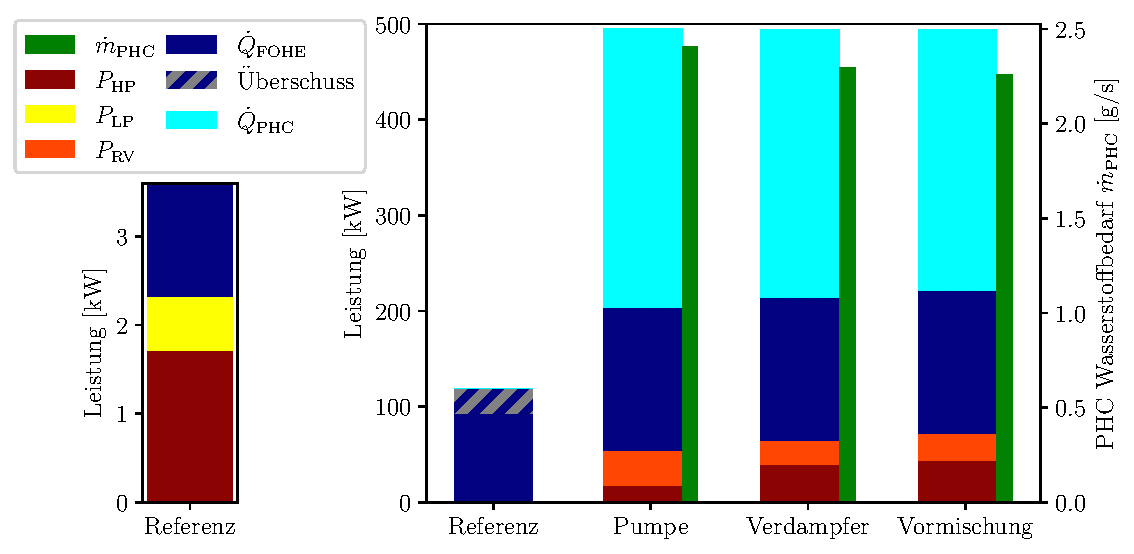
\includegraphics[width=1\linewidth]{4_Abbildungen/2_Hauptteil/Ergebnisse/refcomp.pdf}
  \caption{Betriebsmittelbedarf der Kraftstoffsysteme}
  \label{fig:refcomp}
\end{figure}
\FloatBarrier

Der Betriebsmittelbedarf der Wasserstoff-Kraftstoffsysteme übersteigt den Bedarf des Referenzkraftstoffsystems um einen Faktor von drei. Im Vergleich zum Referenzkraftstoffsystem erfordert das Wasserstoff-Kraftstoffsystem mit Pumpe 22,7-Mal mehr Leistungsentnahme von der Hochdruckwelle und hat einen Wärmefehlbetrag von \SI{278}{\kilo\W}, der durch die parallele Wasserstoffverbrennung gedeckt wird. Bei dem Kraftstoffsystem mit Verdampfer wird sogar das 27,1-Fache an Leistungsentnahme benötigt bei einem Wärmefehlbetrag von \SI{268}{\kilo\W}. Bei dem Kraftstoffsystem mit Vormischung wird das 30,2-Fache an Leistungsentnahme benötigt bei einem Wärmefehlbetrag von nur noch \SI{261}{\kilo\W}. 

Um die Vergleichbarkeit des Kraftstoffverbrauchs sicherzustellen, wird der Energieverbrauch als Produkt aus dem Kraftstoffverbrauch und dem unteren Heizwert bei Normaldruck und einer Temperatur von \SI{298.15}{\K} berechnet.
Abbildung \ref{fig:refenergy} zeigt die Differenz des Energieverbrauchs der Wasserstoff-Kraftstoffsysteme zum Referenzkraftstoffsystem. 

\begin{figure}[ht]
\centering
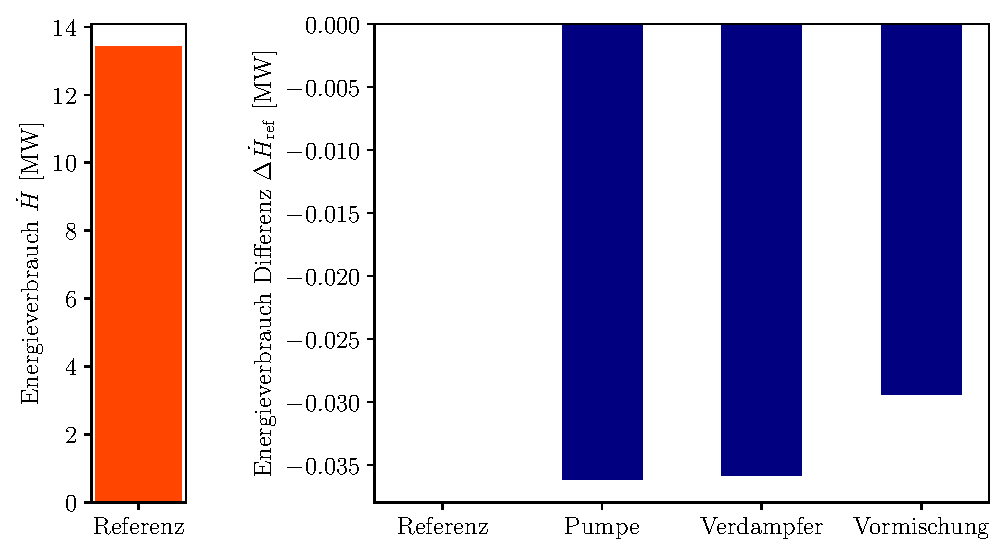
\includegraphics[width=1\linewidth]{4_Abbildungen/2_Hauptteil/Ergebnisse/refenergy.pdf}
  \caption{Energieverbrauch der Kraftstoffsysteme}
  \label{fig:refenergy}
\end{figure}
\FloatBarrier

Trotz des zusätzlichen Betriebsmittelbedarfs verbrauchen die Wasserstoff-Kraftstoffsysteme bis zu $0{,}27\,\%$ weniger Energie. Dies ist auf den höheren Wirkungsgrad des Kreisprozesses des wasserstoffbetriebenen Zyklus zurückzuführen, der durch die abweichenden Abgaseigenschaften begünstigt wird.
%%==============================================================================
\chapter{Diskussion} \label{chap:disk}
%==============================================================================




%==============================================================================
\chapter{Zusammenfassung und Ausblick}
\label{chap:fazit}
%==============================================================================

Der Einsatz wasserstoffbetriebener Fluggasturbinen erfordert Leistungsfähige Kraftstoffsysteme, die den erheblichen Wärmebedarf für die Vorkonditionierung des flüssigen Wasserstoffs decken können. Kenntnis der spezifischen Wärme- und Leistungsanforderungen in den relevanten Betriebspunkten ist dabei essenziell für die angemessene Dimensionierung der Systemkomponenten. Der Fokus dieser Arbeit ist die Entwicklung einer Modellierung zur Abschätzung dieser Anforderungen, insbesondere in Abhängigkeit der durch die Systemauslegung zu bestimmenden Eintrittstemperaturen. 

Im Rahmen dieser Arbeit wurden ein Referenzkraftstoffsystem und drei Wasserstoff-Kraftstoffsysteme entwickelt. Die Modellierung der Kraftstoffsysteme erfolgte anhand von Komponenten- und Stoffmodellen, die auf Basis einer umfassenden Literaturrecherche für den Betriebspunkt eines Verkehrsflugzeugs im Reiseflug parametriert wurden. Diese Modellierung bestimmt den Wärmebedarf, die erforderlichen Pumpen- und Verdichterleistungen sowie den daraus resultierenden Mehrverbrauch in Abhängigkeit von den Auslegungsgrößen.  Zudem ermöglichen die zugrunde liegenden Komponenten- und Stoffmodelle eine flexible Kombination in verschiedenen Anordnungen, um alternative Kraftstoffsystem-Konzepte abzubilden und zu vergleichen.

Die Methodik dieser Arbeit wurde auf ein bekanntes Kraftstoffsystem aus der Literatur angewandt, um die Aussagekraft des Ansatzes zu bestätigen. Das Ergebnis dieser Validierung ergab eine Übereinstimmung mit den Literaturdaten, jedoch nur in Teilen. Der Ursprung dieser Abweichung konnte nicht abschließend geklärt werden. Im Rahmen einer zweidimensionalen Parameterstudie der Wasserstoff-Kraftstoffsysteme konnte ein Zusammenhang zwischen Kraftstoffverbrauch und Wärmeübertrager-Eintrittstemperatur festgestellt werden. In dem Anschließenden Vergleich mit dem Referenzkraftstoffsystem konnte gezeigt werden, dass die Wasserstoff-Kraftstoffsysteme im Reiseflug trotz höherem Wärmebedarf und höherer notwendiger Leistungsentnahme einen geringeren Energieverbrauch ermöglichen. 

Zukünftige Arbeiten könnten sich mit abweichenden Anordnungen der Komponenten der Wasserstoff-Kraftstoffsysteme befassen, insbesondere im Hinblick auf die Integration von Wärmeübertragern und der Rezirkulation, um die Wärmeübertrager-Eintrittstemperatur zu erreichen. Fortgeschrittene Arbeiten könnten sich damit beschäftigen die Modellierung auf Gesamttriebwerksebene in Leistungsrechnungen zu integrieren und die Modellierung durch die Berücksichtigung von transienten und Off-Design-Punkten zu erweitern. Dies würde zudem die Entwicklung einer Regelstrategie für die einzelnen Kraftstoffsystemkomponenten erfordern.



%%% c) Literaturverzeichnis																					
\renewcommand{\baselinestretch}{0.90}\normalsize
\urlstyle{same}
\bibliographystyle{natdin}
\bibliography{Literatur}
\addcontentsline{toc}{chapter}{Literatur}




%%% d) Anhang
\renewcommand{\baselinestretch}{1.00}\normalsize
\appendix




%%% d) ToDo-Notes
\listoftodos																%% Erstellt Liste mit Aufgaben. Zum deaktivieren in der Datei Pakete.tex zwischen den eckigen Klammern disable hinzufügen

\end{document}